% VLDB Journal extended version of the ICLR 2026 PhaseFormer paper.
% Springer svjour3 class, two-column option, as required by the VLDBJ
% submission rules (two-column template, at most 25 pages).
\RequirePackage{fix-cm}
\documentclass[twocolumn,natbib]{svjour3}
\smartqed

\usepackage[T1]{fontenc}
\usepackage{times}
\usepackage[protrusion=true,expansion=true]{microtype}
\usepackage{amsmath,amssymb}
\usepackage{graphicx}
\usepackage{multirow}
\usepackage{booktabs}
\usepackage{xspace}
\usepackage{enumitem}
\usepackage{xcolor}
\usepackage{subcaption}
\usepackage{url}
\usepackage[hidelinks]{hyperref}
\usepackage{xurl}

% Optional math commands from https://github.com/goodfeli/dlbook_notation.
%%%%% NEW MATH DEFINITIONS %%%%%

\usepackage{amsmath,amsfonts,bm}

% Mark sections of captions for referring to divisions of figures
\newcommand{\figleft}{{\em (Left)}}
\newcommand{\figcenter}{{\em (Center)}}
\newcommand{\figright}{{\em (Right)}}
\newcommand{\figtop}{{\em (Top)}}
\newcommand{\figbottom}{{\em (Bottom)}}
\newcommand{\captiona}{{\em (a)}}
\newcommand{\captionb}{{\em (b)}}
\newcommand{\captionc}{{\em (c)}}
\newcommand{\captiond}{{\em (d)}}

% Highlight a newly defined term
\newcommand{\newterm}[1]{{\bf #1}}


% Figure reference, lower-case.
\def\figref#1{figure~\ref{#1}}
% Figure reference, capital. For start of sentence
\def\Figref#1{Figure~\ref{#1}}
\def\twofigref#1#2{figures \ref{#1} and \ref{#2}}
\def\quadfigref#1#2#3#4{figures \ref{#1}, \ref{#2}, \ref{#3} and \ref{#4}}
% Section reference, lower-case.
\def\secref#1{section~\ref{#1}}
% Section reference, capital.
\def\Secref#1{Section~\ref{#1}}
% Reference to two sections.
\def\twosecrefs#1#2{sections \ref{#1} and \ref{#2}}
% Reference to three sections.
\def\secrefs#1#2#3{sections \ref{#1}, \ref{#2} and \ref{#3}}
% Reference to an equation, lower-case.
\def\eqref#1{equation~\ref{#1}}
% Reference to an equation, upper case
\def\Eqref#1{Equation~\ref{#1}}
% A raw reference to an equation---avoid using if possible
\def\plaineqref#1{\ref{#1}}
% Reference to a chapter, lower-case.
\def\chapref#1{chapter~\ref{#1}}
% Reference to an equation, upper case.
\def\Chapref#1{Chapter~\ref{#1}}
% Reference to a range of chapters
\def\rangechapref#1#2{chapters\ref{#1}--\ref{#2}}
% Reference to an algorithm, lower-case.
\def\algref#1{algorithm~\ref{#1}}
% Reference to an algorithm, upper case.
\def\Algref#1{Algorithm~\ref{#1}}
\def\twoalgref#1#2{algorithms \ref{#1} and \ref{#2}}
\def\Twoalgref#1#2{Algorithms \ref{#1} and \ref{#2}}
% Reference to a part, lower case
\def\partref#1{part~\ref{#1}}
% Reference to a part, upper case
\def\Partref#1{Part~\ref{#1}}
\def\twopartref#1#2{parts \ref{#1} and \ref{#2}}

\def\ceil#1{\lceil #1 \rceil}
\def\floor#1{\lfloor #1 \rfloor}
\def\1{\bm{1}}
\newcommand{\train}{\mathcal{D}}
\newcommand{\valid}{\mathcal{D_{\mathrm{valid}}}}
\newcommand{\test}{\mathcal{D_{\mathrm{test}}}}

\def\eps{{\epsilon}}


% Random variables
\def\reta{{\textnormal{$\eta$}}}
\def\ra{{\textnormal{a}}}
\def\rb{{\textnormal{b}}}
\def\rc{{\textnormal{c}}}
\def\rd{{\textnormal{d}}}
\def\re{{\textnormal{e}}}
\def\rf{{\textnormal{f}}}
\def\rg{{\textnormal{g}}}
\def\rh{{\textnormal{h}}}
\def\ri{{\textnormal{i}}}
\def\rj{{\textnormal{j}}}
\def\rk{{\textnormal{k}}}
\def\rl{{\textnormal{l}}}
% rm is already a command, just don't name any random variables m
\def\rn{{\textnormal{n}}}
\def\ro{{\textnormal{o}}}
\def\rp{{\textnormal{p}}}
\def\rq{{\textnormal{q}}}
\def\rr{{\textnormal{r}}}
\def\rs{{\textnormal{s}}}
\def\rt{{\textnormal{t}}}
\def\ru{{\textnormal{u}}}
\def\rv{{\textnormal{v}}}
\def\rw{{\textnormal{w}}}
\def\rx{{\textnormal{x}}}
\def\ry{{\textnormal{y}}}
\def\rz{{\textnormal{z}}}

% Random vectors
\def\rvepsilon{{\mathbf{\epsilon}}}
\def\rvtheta{{\mathbf{\theta}}}
\def\rva{{\mathbf{a}}}
\def\rvb{{\mathbf{b}}}
\def\rvc{{\mathbf{c}}}
\def\rvd{{\mathbf{d}}}
\def\rve{{\mathbf{e}}}
\def\rvf{{\mathbf{f}}}
\def\rvg{{\mathbf{g}}}
\def\rvh{{\mathbf{h}}}
\def\rvu{{\mathbf{i}}}
\def\rvj{{\mathbf{j}}}
\def\rvk{{\mathbf{k}}}
\def\rvl{{\mathbf{l}}}
\def\rvm{{\mathbf{m}}}
\def\rvn{{\mathbf{n}}}
\def\rvo{{\mathbf{o}}}
\def\rvp{{\mathbf{p}}}
\def\rvq{{\mathbf{q}}}
\def\rvr{{\mathbf{r}}}
\def\rvs{{\mathbf{s}}}
\def\rvt{{\mathbf{t}}}
\def\rvu{{\mathbf{u}}}
\def\rvv{{\mathbf{v}}}
\def\rvw{{\mathbf{w}}}
\def\rvx{{\mathbf{x}}}
\def\rvy{{\mathbf{y}}}
\def\rvz{{\mathbf{z}}}

% Elements of random vectors
\def\erva{{\textnormal{a}}}
\def\ervb{{\textnormal{b}}}
\def\ervc{{\textnormal{c}}}
\def\ervd{{\textnormal{d}}}
\def\erve{{\textnormal{e}}}
\def\ervf{{\textnormal{f}}}
\def\ervg{{\textnormal{g}}}
\def\ervh{{\textnormal{h}}}
\def\ervi{{\textnormal{i}}}
\def\ervj{{\textnormal{j}}}
\def\ervk{{\textnormal{k}}}
\def\ervl{{\textnormal{l}}}
\def\ervm{{\textnormal{m}}}
\def\ervn{{\textnormal{n}}}
\def\ervo{{\textnormal{o}}}
\def\ervp{{\textnormal{p}}}
\def\ervq{{\textnormal{q}}}
\def\ervr{{\textnormal{r}}}
\def\ervs{{\textnormal{s}}}
\def\ervt{{\textnormal{t}}}
\def\ervu{{\textnormal{u}}}
\def\ervv{{\textnormal{v}}}
\def\ervw{{\textnormal{w}}}
\def\ervx{{\textnormal{x}}}
\def\ervy{{\textnormal{y}}}
\def\ervz{{\textnormal{z}}}

% Random matrices
\def\rmA{{\mathbf{A}}}
\def\rmB{{\mathbf{B}}}
\def\rmC{{\mathbf{C}}}
\def\rmD{{\mathbf{D}}}
\def\rmE{{\mathbf{E}}}
\def\rmF{{\mathbf{F}}}
\def\rmG{{\mathbf{G}}}
\def\rmH{{\mathbf{H}}}
\def\rmI{{\mathbf{I}}}
\def\rmJ{{\mathbf{J}}}
\def\rmK{{\mathbf{K}}}
\def\rmL{{\mathbf{L}}}
\def\rmM{{\mathbf{M}}}
\def\rmN{{\mathbf{N}}}
\def\rmO{{\mathbf{O}}}
\def\rmP{{\mathbf{P}}}
\def\rmQ{{\mathbf{Q}}}
\def\rmR{{\mathbf{R}}}
\def\rmS{{\mathbf{S}}}
\def\rmT{{\mathbf{T}}}
\def\rmU{{\mathbf{U}}}
\def\rmV{{\mathbf{V}}}
\def\rmW{{\mathbf{W}}}
\def\rmX{{\mathbf{X}}}
\def\rmY{{\mathbf{Y}}}
\def\rmZ{{\mathbf{Z}}}

% Elements of random matrices
\def\ermA{{\textnormal{A}}}
\def\ermB{{\textnormal{B}}}
\def\ermC{{\textnormal{C}}}
\def\ermD{{\textnormal{D}}}
\def\ermE{{\textnormal{E}}}
\def\ermF{{\textnormal{F}}}
\def\ermG{{\textnormal{G}}}
\def\ermH{{\textnormal{H}}}
\def\ermI{{\textnormal{I}}}
\def\ermJ{{\textnormal{J}}}
\def\ermK{{\textnormal{K}}}
\def\ermL{{\textnormal{L}}}
\def\ermM{{\textnormal{M}}}
\def\ermN{{\textnormal{N}}}
\def\ermO{{\textnormal{O}}}
\def\ermP{{\textnormal{P}}}
\def\ermQ{{\textnormal{Q}}}
\def\ermR{{\textnormal{R}}}
\def\ermS{{\textnormal{S}}}
\def\ermT{{\textnormal{T}}}
\def\ermU{{\textnormal{U}}}
\def\ermV{{\textnormal{V}}}
\def\ermW{{\textnormal{W}}}
\def\ermX{{\textnormal{X}}}
\def\ermY{{\textnormal{Y}}}
\def\ermZ{{\textnormal{Z}}}

% Vectors
\def\vzero{{\bm{0}}}
\def\vone{{\bm{1}}}
\def\vmu{{\bm{\mu}}}
\def\vtheta{{\bm{\theta}}}
\def\va{{\bm{a}}}
\def\vb{{\bm{b}}}
\def\vc{{\bm{c}}}
\def\vd{{\bm{d}}}
\def\ve{{\bm{e}}}
\def\vf{{\bm{f}}}
\def\vg{{\bm{g}}}
\def\vh{{\bm{h}}}
\def\vi{{\bm{i}}}
\def\vj{{\bm{j}}}
\def\vk{{\bm{k}}}
\def\vl{{\bm{l}}}
\def\vm{{\bm{m}}}
\def\vn{{\bm{n}}}
\def\vo{{\bm{o}}}
\def\vp{{\bm{p}}}
\def\vq{{\bm{q}}}
\def\vr{{\bm{r}}}
\def\vs{{\bm{s}}}
\def\vt{{\bm{t}}}
\def\vu{{\bm{u}}}
\def\vv{{\bm{v}}}
\def\vw{{\bm{w}}}
\def\vx{{\bm{x}}}
\def\vy{{\bm{y}}}
\def\vz{{\bm{z}}}

% Elements of vectors
\def\evalpha{{\alpha}}
\def\evbeta{{\beta}}
\def\evepsilon{{\epsilon}}
\def\evlambda{{\lambda}}
\def\evomega{{\omega}}
\def\evmu{{\mu}}
\def\evpsi{{\psi}}
\def\evsigma{{\sigma}}
\def\evtheta{{\theta}}
\def\eva{{a}}
\def\evb{{b}}
\def\evc{{c}}
\def\evd{{d}}
\def\eve{{e}}
\def\evf{{f}}
\def\evg{{g}}
\def\evh{{h}}
\def\evi{{i}}
\def\evj{{j}}
\def\evk{{k}}
\def\evl{{l}}
\def\evm{{m}}
\def\evn{{n}}
\def\evo{{o}}
\def\evp{{p}}
\def\evq{{q}}
\def\evr{{r}}
\def\evs{{s}}
\def\evt{{t}}
\def\evu{{u}}
\def\evv{{v}}
\def\evw{{w}}
\def\evx{{x}}
\def\evy{{y}}
\def\evz{{z}}

% Matrix
\def\mA{{\bm{A}}}
\def\mB{{\bm{B}}}
\def\mC{{\bm{C}}}
\def\mD{{\bm{D}}}
\def\mE{{\bm{E}}}
\def\mF{{\bm{F}}}
\def\mG{{\bm{G}}}
\def\mH{{\bm{H}}}
\def\mI{{\bm{I}}}
\def\mJ{{\bm{J}}}
\def\mK{{\bm{K}}}
\def\mL{{\bm{L}}}
\def\mM{{\bm{M}}}
\def\mN{{\bm{N}}}
\def\mO{{\bm{O}}}
\def\mP{{\bm{P}}}
\def\mQ{{\bm{Q}}}
\def\mR{{\bm{R}}}
\def\mS{{\bm{S}}}
\def\mT{{\bm{T}}}
\def\mU{{\bm{U}}}
\def\mV{{\bm{V}}}
\def\mW{{\bm{W}}}
\def\mX{{\bm{X}}}
\def\mY{{\bm{Y}}}
\def\mZ{{\bm{Z}}}
\def\mBeta{{\bm{\beta}}}
\def\mPhi{{\bm{\Phi}}}
\def\mLambda{{\bm{\Lambda}}}
\def\mSigma{{\bm{\Sigma}}}

% Tensor
\DeclareMathAlphabet{\mathsfit}{\encodingdefault}{\sfdefault}{m}{sl}
\SetMathAlphabet{\mathsfit}{bold}{\encodingdefault}{\sfdefault}{bx}{n}
\providecommand{\tens}[1]{\bm{\mathsfit{#1}}}
\def\tA{{\tens{A}}}
\def\tB{{\tens{B}}}
\def\tC{{\tens{C}}}
\def\tD{{\tens{D}}}
\def\tE{{\tens{E}}}
\def\tF{{\tens{F}}}
\def\tG{{\tens{G}}}
\def\tH{{\tens{H}}}
\def\tI{{\tens{I}}}
\def\tJ{{\tens{J}}}
\def\tK{{\tens{K}}}
\def\tL{{\tens{L}}}
\def\tM{{\tens{M}}}
\def\tN{{\tens{N}}}
\def\tO{{\tens{O}}}
\def\tP{{\tens{P}}}
\def\tQ{{\tens{Q}}}
\def\tR{{\tens{R}}}
\def\tS{{\tens{S}}}
\def\tT{{\tens{T}}}
\def\tU{{\tens{U}}}
\def\tV{{\tens{V}}}
\def\tW{{\tens{W}}}
\def\tX{{\tens{X}}}
\def\tY{{\tens{Y}}}
\def\tZ{{\tens{Z}}}


% Graph
\def\gA{{\mathcal{A}}}
\def\gB{{\mathcal{B}}}
\def\gC{{\mathcal{C}}}
\def\gD{{\mathcal{D}}}
\def\gE{{\mathcal{E}}}
\def\gF{{\mathcal{F}}}
\def\gG{{\mathcal{G}}}
\def\gH{{\mathcal{H}}}
\def\gI{{\mathcal{I}}}
\def\gJ{{\mathcal{J}}}
\def\gK{{\mathcal{K}}}
\def\gL{{\mathcal{L}}}
\def\gM{{\mathcal{M}}}
\def\gN{{\mathcal{N}}}
\def\gO{{\mathcal{O}}}
\def\gP{{\mathcal{P}}}
\def\gQ{{\mathcal{Q}}}
\def\gR{{\mathcal{R}}}
\def\gS{{\mathcal{S}}}
\def\gT{{\mathcal{T}}}
\def\gU{{\mathcal{U}}}
\def\gV{{\mathcal{V}}}
\def\gW{{\mathcal{W}}}
\def\gX{{\mathcal{X}}}
\def\gY{{\mathcal{Y}}}
\def\gZ{{\mathcal{Z}}}

% Sets
\def\sA{{\mathbb{A}}}
\def\sB{{\mathbb{B}}}
\def\sC{{\mathbb{C}}}
\def\sD{{\mathbb{D}}}
% Don't use a set called E, because this would be the same as our symbol
% for expectation.
\def\sF{{\mathbb{F}}}
\def\sG{{\mathbb{G}}}
\def\sH{{\mathbb{H}}}
\def\sI{{\mathbb{I}}}
\def\sJ{{\mathbb{J}}}
\def\sK{{\mathbb{K}}}
\def\sL{{\mathbb{L}}}
\def\sM{{\mathbb{M}}}
\def\sN{{\mathbb{N}}}
\def\sO{{\mathbb{O}}}
\def\sP{{\mathbb{P}}}
\def\sQ{{\mathbb{Q}}}
\def\sR{{\mathbb{R}}}
\def\sS{{\mathbb{S}}}
\def\sT{{\mathbb{T}}}
\def\sU{{\mathbb{U}}}
\def\sV{{\mathbb{V}}}
\def\sW{{\mathbb{W}}}
\def\sX{{\mathbb{X}}}
\def\sY{{\mathbb{Y}}}
\def\sZ{{\mathbb{Z}}}

% Entries of a matrix
\def\emLambda{{\Lambda}}
\def\emA{{A}}
\def\emB{{B}}
\def\emC{{C}}
\def\emD{{D}}
\def\emE{{E}}
\def\emF{{F}}
\def\emG{{G}}
\def\emH{{H}}
\def\emI{{I}}
\def\emJ{{J}}
\def\emK{{K}}
\def\emL{{L}}
\def\emM{{M}}
\def\emN{{N}}
\def\emO{{O}}
\def\emP{{P}}
\def\emQ{{Q}}
\def\emR{{R}}
\def\emS{{S}}
\def\emT{{T}}
\def\emU{{U}}
\def\emV{{V}}
\def\emW{{W}}
\def\emX{{X}}
\def\emY{{Y}}
\def\emZ{{Z}}
\def\emSigma{{\Sigma}}

% entries of a tensor
% Same font as tensor, without \bm wrapper
\newcommand{\etens}[1]{\mathsfit{#1}}
\def\etLambda{{\etens{\Lambda}}}
\def\etA{{\etens{A}}}
\def\etB{{\etens{B}}}
\def\etC{{\etens{C}}}
\def\etD{{\etens{D}}}
\def\etE{{\etens{E}}}
\def\etF{{\etens{F}}}
\def\etG{{\etens{G}}}
\def\etH{{\etens{H}}}
\def\etI{{\etens{I}}}
\def\etJ{{\etens{J}}}
\def\etK{{\etens{K}}}
\def\etL{{\etens{L}}}
\def\etM{{\etens{M}}}
\def\etN{{\etens{N}}}
\def\etO{{\etens{O}}}
\def\etP{{\etens{P}}}
\def\etQ{{\etens{Q}}}
\def\etR{{\etens{R}}}
\def\etS{{\etens{S}}}
\def\etT{{\etens{T}}}
\def\etU{{\etens{U}}}
\def\etV{{\etens{V}}}
\def\etW{{\etens{W}}}
\def\etX{{\etens{X}}}
\def\etY{{\etens{Y}}}
\def\etZ{{\etens{Z}}}

% The true underlying data generating distribution
\newcommand{\pdata}{p_{\rm{data}}}
% The empirical distribution defined by the training set
\newcommand{\ptrain}{\hat{p}_{\rm{data}}}
\newcommand{\Ptrain}{\hat{P}_{\rm{data}}}
% The model distribution
\newcommand{\pmodel}{p_{\rm{model}}}
\newcommand{\Pmodel}{P_{\rm{model}}}
\newcommand{\ptildemodel}{\tilde{p}_{\rm{model}}}
% Stochastic autoencoder distributions
\newcommand{\pencode}{p_{\rm{encoder}}}
\newcommand{\pdecode}{p_{\rm{decoder}}}
\newcommand{\precons}{p_{\rm{reconstruct}}}

\newcommand{\laplace}{\mathrm{Laplace}} % Laplace distribution

\newcommand{\E}{\mathbb{E}}
\newcommand{\Ls}{\mathcal{L}}
\newcommand{\R}{\mathbb{R}}
\newcommand{\emp}{\tilde{p}}
\newcommand{\lr}{\alpha}
\newcommand{\reg}{\lambda}
\newcommand{\rect}{\mathrm{rectifier}}
\newcommand{\softmax}{\mathrm{softmax}}
\newcommand{\sigmoid}{\sigma}
\newcommand{\softplus}{\zeta}
\newcommand{\KL}{D_{\mathrm{KL}}}
\newcommand{\Var}{\mathrm{Var}}
\newcommand{\standarderror}{\mathrm{SE}}
\newcommand{\Cov}{\mathrm{Cov}}
% Wolfram Mathworld says $L^2$ is for function spaces and $\ell^2$ is for vectors
% But then they seem to use $L^2$ for vectors throughout the site, and so does
% wikipedia.
\newcommand{\normlzero}{L^0}
\newcommand{\normlone}{L^1}
\newcommand{\normltwo}{L^2}
\newcommand{\normlp}{L^p}
\newcommand{\normmax}{L^\infty}

\newcommand{\parents}{Pa} % See usage in notation.tex. Chosen to match Daphne's book.

\DeclareMathOperator*{\argmax}{arg\,max}
\DeclareMathOperator*{\argmin}{arg\,min}

\DeclareMathOperator{\sign}{sign}
\DeclareMathOperator{\Tr}{Tr}
\let\ab\allowbreak


% ---------------------------------------------------------------------------
% Change marking for the journal extension.
% Every passage that is new or changed relative to the ICLR 2026 version is
% wrapped in \blue{...}. Set \showchangestrue to false (\showchangesfalse)
% for a clean copy. \blue accepts several paragraphs, lists, theorems and
% section headings; inside a float, wrap the float's content, not the float.
% ---------------------------------------------------------------------------
\newif\ifshowchanges
\showchangestrue
\ifshowchanges
\newcommand{\blue}[1]{{\color{blue}#1}}
\else
\newcommand{\blue}[1]{#1}
\fi

% Macros inherited from the conference version.
\newcommand{\eg}{\textit{e.g.}\xspace}
\newcommand{\ie}{\textit{i.e.}\xspace}
\newcommand{\etc}{etc.\xspace}
\newcommand{\aka}{\textit{a.k.a.}\xspace}
\newcommand{\versus}{\emph{vs.}\xspace}

\newcommand\tabref[1]{Tab.~\ref{#1}}
\renewcommand\secref[1]{Sec.~\ref{#1}}
\renewcommand\figref[1]{Fig.~\ref{#1}}
\newcommand\appref[1]{Appendix~\ref{#1}}
\newcommand\equref[1]{Eq.~(\ref{#1})}
\newcommand\thmref[1]{Theorem~\ref{#1}}
\newcommand\lemmaref[1]{Lemma~\ref{#1}}

\newcommand{\fakeparagraph}[1]{\vspace{1mm}\noindent\textbf{#1.}}
\newcommand{\sysname}{PhaseFormer\xspace}
\newcommand{\sysL}{PhaseFormer-L\xspace}
\newcommand{\sysLA}{PhaseFormer-LA\xspace}
\newcommand{\codeurl}{https://github.com/neumyor/PhaseFormer_TSL}

% Best / second-best marks of the conference tables. The second-best color is
% kept separate from \blue so that it is not read as a change mark.
\definecolor{secondcolor}{RGB}{0,90,160}
\newcommand{\red}[1]{\textcolor{red}{#1}}
\newcommand{\best}[1]{\red{\textbf{#1}}}
\newcommand{\second}[1]{\textcolor{secondcolor}{\underline{#1}}}
% Passages revised during the ICLR rebuttal are ordinary text here.
\newcommand{\revised}[1]{#1}
\newcommand{\TODO}[1]{\textbf{\color{red}{[TODO: #1]}}}
% Placeholder for results of the final PhaseFormer-LA runs.
\newcommand{\tbd}[1]{{\color{red}[#1]}}

% Notation for the extension (Sections 3, 5 and 6).
\newcommand{\Lp}{L_{\text{phase}}}
\newcommand{\Pin}{P_{\text{in}}}
\newcommand{\Pout}{P_{\text{out}}}
\newcommand{\lev}{\operatorname{lev}}
\newcommand{\LN}{\operatorname{LN}}
\newcommand{\one}{\mathbf 1}

% svjour3 provides theorem, lemma, corollary, proposition, definition,
% remark and the proof environment. Only the missing ones are added.
\spnewtheorem{assumption}{Assumption}{\bfseries}{\itshape}

\journalname{The VLDB Journal}

% Narrow two-column measure: allow extra interword stretch before overfull lines.
\setlength{\emergencystretch}{1.5em}

\begin{document}

\title{PhaseFormer: \blue{Efficient Phase-Based Forecasting for Spatio-Temporal Data Beyond Stable Cycles}%
\thanks{\blue{This article is an extended version of the conference paper ``PhaseFormer: From Patches to Phases for Efficient and Effective Time Series Forecasting'' published at ICLR 2026~\citep{niu2026phaseformer}. The new material is summarized at the end of Section~\ref{sec:intro}.}}}

\author{Yiming Niu \and Jinliang Deng \and Yongxin Tong}

\authorrunning{Y. Niu, J. Deng, Y. Tong}

\institute{Yiming Niu and Jinliang Deng contributed equally to this work. Yongxin Tong is the corresponding author. \at
Yiming Niu, Yongxin Tong \at
State Key Laboratory of Complex \& Critical Software Environment, Beihang University, Beijing, China \\
\email{\{yimingniu, yxtong\}@buaa.edu.cn}
\and
Jinliang Deng \at
State Key Laboratory of Complex \& Critical Software Environment, Beihang University, Beijing, China; Research Institute of Trustworthy Autonomous Systems, Southern University of Science and Technology, Shenzhen, China \\
\email{jinliangdeng9588@gmail.com}}

\date{Received: date / Accepted: date}

\maketitle

\begin{abstract}
\blue{Sensor-network forecasting must serve every sensor at every update, so efficiency matters as much as accuracy. Sensor streams are strongly periodic; how a forecaster tokenizes them determines what exploiting periodicity costs. Patch tokens of consecutive values change whenever the cycle shape changes; covering this variability requires a high-dimensional representation that network-scale deployment cannot afford. We instead tokenize by phase: each token holds the values at one within-cycle offset across cycles. Under a shape change shared by all cycles, the phase-token subspace provably stays invariant up to noise, while the patch-token subspace shifts. PhaseFormer exploits this stability with few parameters: phase tokens share one low-dimensional embedding and interact through a few routers. This stability does not extend to drifts in cycle level or level-dependent amplitude. We prove that PhaseFormer follows such drifts only within two bounds computable from its weights, on forecast level and within-cycle amplitude, and that under standard seasonal models the remainder has a simple structure. PhaseFormer-LA (Level--Amplitude) adds two components derived from this structure: a gated low-rank branch forecasting the level from cycle means, and a modulation scaling the cycle shape with the level while provably leaving the forecast level unchanged. With about 1,000 parameters, over 99.8\% fewer than PatchTST and Crossformer, PhaseFormer is the most accurate of eleven models on four of seven benchmarks and within 4\% of the best elsewhere. \tbd{Where these bounds are exceeded, PhaseFormer-LA lowers the error by up to Y\%, otherwise changing it by at most Z\%.} Code is available at \url{\codeurl}.}
\keywords{Time series forecasting \and \blue{Spatio-temporal data} \and Periodicity \and Phase tokenization \and \blue{Non-stationarity} \and Efficient models}
\end{abstract}

\section{Introduction}
\label{sec:intro}
Time series forecasting underpins decision-making across diverse domains such as finance, energy, climate science, and healthcare, playing a pivotal role in tasks including weather forecasting~\citep{weathernature2025,wu2021autoformer}, energy consumption planning~\citep{lai2018energy,alvarez2010energy,cheng2021windturbine}, traffic scheduling~\citep{cirstea2022towardstraffic,cirstea2021enhancenet,wu2021autocts}.
\blue{Many of these series are spatio-temporal: they are produced by large networks of sensors, such as loop detectors on a road network or smart meters on a power grid, and a forecasting system must serve every sensor of the network continuously. In this setting the cost of a model is multiplied by the number of sensors and by the frequency of re-forecasting, so efficiency and scalability are first-class requirements alongside accuracy~\citep{lai2023lightcts}.}
In recent years, deep learning has demonstrated promising potential in this field by leveraging end-to-end modeling and powerful representational capacity to extrapolate from history to future trends.

A central inductive bias in forecasting models is periodicity--the recurring temporal structure inherent in many real-world time series.
Periodicity is ubiquitous in practice, appearing in domains ranging from urban traffic flow to cloud resource utilization and other workloads, making periodicity-aware modeling broadly applicable~\citep{deng2024disentangling, xia2025timeemb}.
Recent advances exploited this property by segmenting sequences into patch tokens, potentially aligned with cycles, prior to processing by the crafted models~\citep{nie2023patchtst, zhang2023crossformer, huang2025timebase, tang2025unlocking}.
For instance, \cite{nie2023patchtst} applied Transformer to tokenized time series to capture temporal correlations within and between cycles, while \cite{zhang2023crossformer} extended this paradigm by modeling cross-dimension dependencies and cross-scale interactions.

\begin{figure*}[t]
  \centering
  \begin{subfigure}[t]{0.49\textwidth}
    \centering
    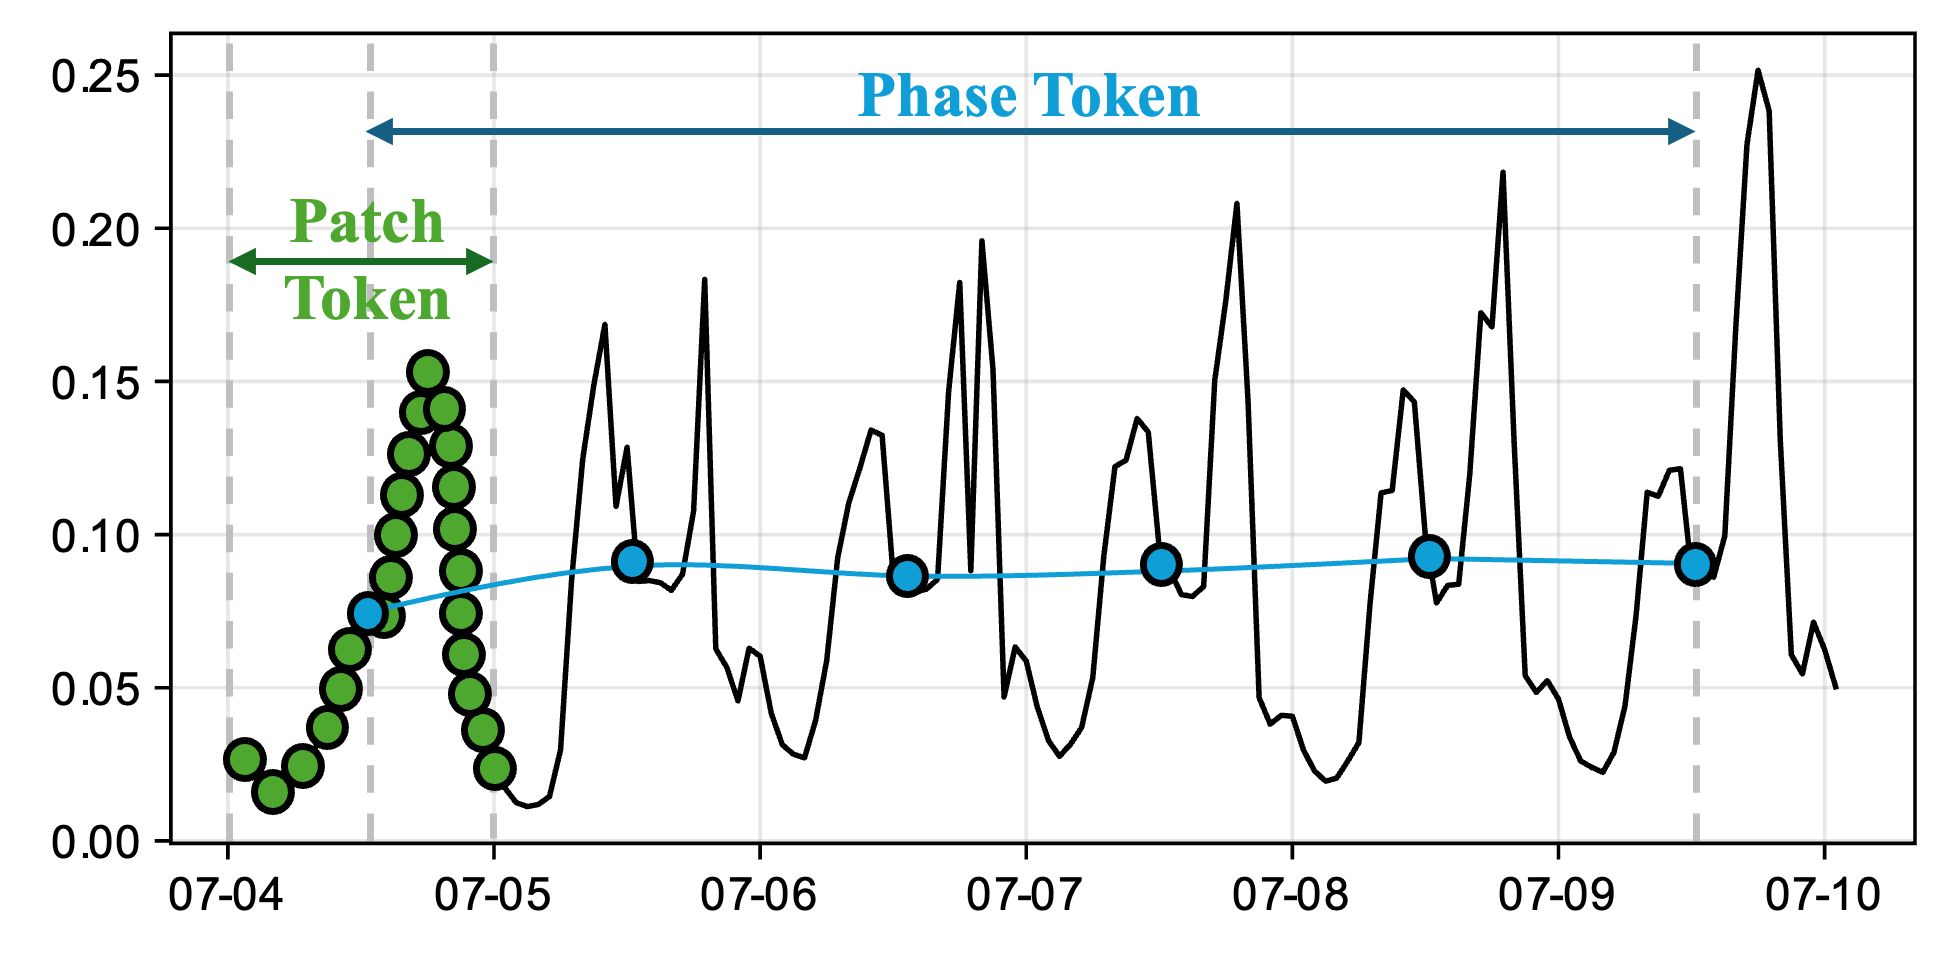
\includegraphics[width=\linewidth]{figures/phase_token.png}
    \caption{Patch Token vs. Phase Token.}
    \label{fig:phase_token}
  \end{subfigure}
  \hfill
  \begin{subfigure}[t]{0.49\textwidth}
    \centering
    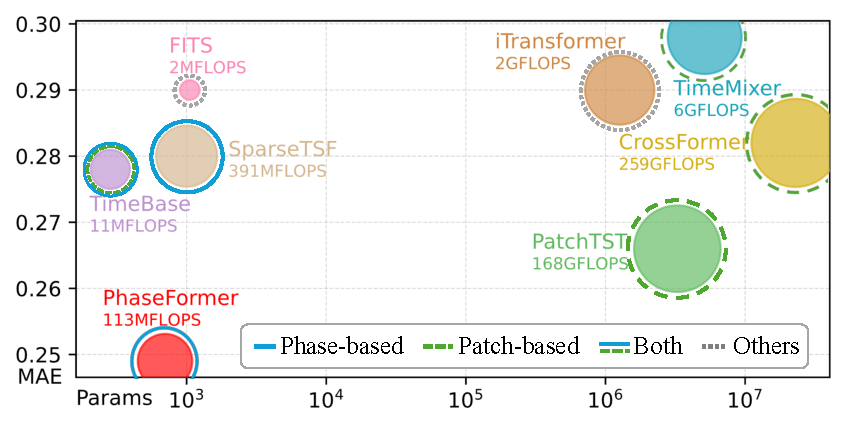
\includegraphics[width=\linewidth]{figures/efficiency_plot.pdf}
    \caption{Model Accuracy and Efficiency Comparison.}
    \label{fig:efficiency_plot}
  \end{subfigure}
  \caption{Comparison between patch-based and phase-based representations for time-series forecasting. (a) illustrates the difference in tokenization. (b) provides a joint evaluation of model accuracy, parameter scale, and computational overhead on the Traffic dataset, using an input length of 720 steps and predicting 96 future steps, where the marker size denotes the FLOPs.}
  \label{fig:introduction}
\end{figure*}

Despite their effectiveness, patch-based approaches struggle to scale efficiently to large and complex datasets~\citep{nie2023patchtst, zhang2023crossformer,tang2025unlocking}.
\emph{We attribute this poor scalability to the substantial variability of cycle patterns in real-world scenarios}.
This variability stems from dynamic external factors, which continuously shift the cycle patterns. For instance, traffic flow patterns may evolve as new infrastructure is introduced, while electricity demand can change with adjustments in work schedules~\citep{shao2025hutformer, shao2025hyperd, zhou2025feddis}.
This variability forces models to construct a high-dimensional representation space to faithfully accommodate the broadened distribution, which inevitably inflates both parameter counts and computational costs~\citep{shao2025blast}.
Additionally, these methods also struggle to generalize under such varying behavior, resulting in unreliable forecasts for samples beyond training data.

To address this challenge, we introduce a phase-based perspective that focuses on values aligned at the same offset across successive cycles. From this perspective, the dynamics of a time series are characterized by the cross-period trends of each phase--captured as phase tokens--while disregarding the full cyclic behavior. As illustrated in Fig.~\ref{fig:phase_token}, phase tokens exhibit significantly lower variability than patch tokens, enabling more efficient and generalizable representation, which in turn makes \sysname well suited for resource-constrained environments.
Importantly, excluding cycle patterns has minimal impact on forecasting effectiveness, since the cyclic behaviors remain locally stable and thus require little effort to predict. We study and verify these properties in depth in Sec.~\ref{sec:motivations} using real-world data, showing the stationarity and compactness of the feature space offered by phase tokenization.

Building on these insights, we propose Phase-based Routing Transformer, abbreviated as \textbf{\sysname}, which reframes time series as a collection of phase tokens and casts step-wise prediction as phase-wise prediction. Specifically, \sysname (i) aligns and extracts phase tokens from the input sequence and maps them into a shared low-dimensional latent space, (ii) employs a lightweight routing mechanism to enable efficient communication across phases, and (iii) applies a shared predictor to project the latent representations into forecasts for each phase. Extensive experiments demonstrate that, compared with PatchTST~\citep{nie2023patchtst} and Crossformer~\citep{zhang2023crossformer}, \sysname achieves over \textbf{99.9\%} reduction in both parameter count and computational cost, while delivering consistent improvements in prediction accuracy across all seven benchmark datasets, as illustrated by the Traffic dataset in Fig.~\ref{fig:efficiency_plot}.
Moreover, in contrast to methods with comparable efficiency such as SparseTSF~\citep{lin2024sparsetsf} and TimeBase~\citep{huang2025timebase}, \sysname significantly enhances predictive effectiveness, particularly on large and complex datasets.
Finally, we conduct a comprehensive analysis of different configurations to reveal the necessity of the constructed components and the effects of various hyperparameters.

\blue{
\fakeparagraph{Beyond stable cycles}
The conference version of this work~\citep{niu2026phaseformer} explained the efficiency of phase tokens with a stability theorem: when the recurring shape of a cycle is transformed in the same way in every cycle, the phase subspace does not move, whereas the patch subspace does. This covers changes \emph{along the phase axis} of the folded series. Real sensor streams also change \emph{along the cycle axis}: the level of a road segment's daily profile drifts from week to week, and the amplitude of that profile grows and shrinks with the level, as in the classical multiplicative seasonality of Holt--Winters~\citep{winters1960forecasting}. Such changes add new directions to the phase subspace, so they fall outside the conference theorem. The conference version left them as its main limitation: \sysname ``assumes locally stable periodicity'', and modeling ``non-stationarity and complex drifts'' was named as future work.

In this extended version, we close this gap theoretically and architecturally while keeping the efficiency that motivates phase tokens. We show that \sysname is not blind to cycle-axis changes: a level shift passes exactly through the routing layer, and the architecture can approximate the Bayes forecast of a seasonal random-walk model. Its capacity is, however, bounded by an \emph{envelope} that is fixed by the final layer normalization and can be read from the trained weights. We prove two such envelopes, one for the cycle level and one for a level-dependent amplitude, and show that what lies outside each envelope has a simple structure. The unmodeled level acts only through a few fixed horizon profiles, so a rank-3 linear branch on cycle means can carry it. The unmodeled amplitude is a bilinear product of level and shape, so a centered multiplicative modulation of the phase latent can carry it, and we prove that this modulation leaves every future cycle mean unchanged, so it does not disturb the level guarantees. The resulting model, \textbf{\sysLA}, keeps the conference architecture unchanged and adds at most a few hundred parameters, independent of the forecast horizon.
}

Our contributions are as follows:

\begin{enumerate}[leftmargin=2em]
\item We introduce a phase-based perspective that aligns values across cycles for the characterization of long-term time series, empirically and theoretically demonstrating improved feature stationarity and compactness over the patch-based perspective.

\item We propose \sysname, a lightweight forecasting model that reframes time series as phase tokens, maps them into a shared latent space, and employs a low-rank routing mechanism specifically designed around phase tokens to enable efficient phase-wise forecasting.

\item Extensive experiments are conducted to showcase that \sysname achieves substantial efficiency gains while consistently improving forecasting accuracy, establishing a superior efficiency–effectiveness trade-off across diverse benchmarks.

\blue{\item We characterize the limits of phase tokenization under cycle-axis changes. We prove a capability result and two envelope theorems, for the level and for the amplitude of cycles, and two complement theorems that identify the minimal structure needed beyond each envelope (Section~\ref{sec:theory}).}

\blue{\item We derive \sysLA from these results: a rank-3 level branch on cycle means with fixed horizon profiles, and a centered amplitude modulation that provably preserves every future cycle mean. Both add at most a few hundred parameters (Section~\ref{sec:extension}).}

\blue{\item We provide a data-centric analysis of level--amplitude coupling on seven benchmarks, which shows that the coupling is present in all of them and is strongest in the traffic and electricity sensor networks, together with synthetic and real-data experiments that test each step of the theory (Section~\ref{sec:ext_exp}).}
\end{enumerate}

\blue{
\fakeparagraph{Relation to the conference version}
Sections~\ref{sec:motivations} and~\ref{sec:method} and Sections~\ref{sec:exp_main}--\ref{sec:exp_case} follow the conference version~\citep{niu2026phaseformer}, with editorial changes. Sections~\ref{sec:theory}, \ref{sec:extension} and~\ref{sec:ext_exp}, the extended related work, the discussion of limitations, and Appendices~\ref{app:proofs}--\ref{app:ext_results} are new. All changes relative to the conference version are marked in blue in this manuscript.
}

\section{\blue{Related Work}}
\label{sec:related}

\blue{
The shape, the level and the amplitude of a periodic series have each been modeled before, but in separate lines of work. Decomposition separates a trend, tokens and cross-cycle models capture the cycle shape, and normalization removes and restores the level and the scale; in none of them does the amplitude have a token of its own, driven by the level. We review each line by what it covers. Where a line leaves two kinds of information mixed, its network must grow to separate them; where it leaves one out, its forecast loses accuracy. \sysplus covers all three with its tokens, and this coverage is what lets it be small. We close with forecasting at the scale of a sensor network, where this matters most.

\fakeparagraph{Decomposition}
Decomposing a series into interpretable parts is a long tradition. Classical methods separate a trend, a seasonal component and a remainder, by local regression in STL~\citep{cleveland1990stl} or by exponential smoothing in Holt--Winters forecasting~\citep{holt2004forecasting,winters1960forecasting,hyndman2021fpp3}, whose multiplicative form scales the seasonal component with the level. Deep forecasters build the split into their architecture. Autoformer~\citep{wu2021autoformer} and FEDformer~\citep{zhou2022fedformer} separate a moving-average trend, a mixture of moving averages in FEDformer, from a seasonal part inside every layer, and model the seasonal part with auto-correlation or frequency-domain attention. DLinear~\citep{zeng2023dlinear} applies one linear map to each part. TimeMixer~\citep{timemixer24} downsamples the series to several scales, decomposes each scale into seasonal and trend parts, mixes the seasonal parts from fine to coarse and the trend parts from coarse to fine, and sums the forecasts of one predictor per scale. The interpretable N-BEATS~\citep{oreshkin2020nbeats} expands the forecast in polynomial trend and Fourier seasonal bases, and CycleNet~\citep{lin2024cyclenet} learns one recurrent cycle per channel, fixed after training, and forecasts the residual with a separate model. These designs share the premise of this paper, that the parts of a series should not be learned in one undifferentiated representation.

\fakeparagraph{Where decomposition falls short}
In the terms of the form $X\approx\ell\,\one^\top+a\,s^\top$ of Section~\ref{sec:mot_tokens}, the trend of these deep decompositions stands in for the level, the seasonal part or the learned cycle holds the shape, and the amplitude of each cycle is left inside the seasonal part or the residual, with no component of its own. They therefore cover the three kinds of information only partly, in three respects. First, they split the series along time, not into its cycles: a level that one number per cycle describes is carried by one value per time step, which the trend model must forecast step by step. Even the coarsest scale of TimeMixer comes from downsampling by fixed factors that the period does not set, so its trend remains a curve over time rather than one level per cycle. Second, they add the parts, and nothing ties the seasonal swing to the trend, so the seasonal model must learn the coupling from examples, level by level; TimeMixer adds its parts twice, when it recombines the seasonal and trend parts at each scale and when it sums the forecasts of its per-scale predictors. The multiplicative Holt--Winters model ties the swing to the level, but in a fixed proportion and through a per-series recursion with a few smoothing constants, not through a coupling learned by a forecaster that serves every sensor. Third, the network that receives each part must untangle whatever the split leaves mixed, and it grows accordingly; where it is a single linear map, as in DLinear, it cannot separate what stays mixed, and the forecast pays in accuracy instead. Partial coverage thus forces a choice between capacity and accuracy.

\sysplus instead represents the folded window by one token for each kind of information: one level per cycle, an amplitude driven by the level, and phase tokens that carry the shape. Its level pathway combines a few fixed horizon profiles, as the trend basis of N-BEATS combines low-degree polynomials, and its amplitude pathway scales the cycle shape with the level while provably leaving every future cycle mean unchanged (Proposition~\ref{prop:modulation}). Each pathway forecasts one kind of information in its low-dimensional form and stays small (Section~\ref{sec:theory}). Where TimeMixer adds scales and predictors, \sysplus adds one number per cycle and a level-driven amplitude factor: it is the full coverage of the shape, the level and the amplitude, not a restriction of the model, that lets it be small.

\fakeparagraph{Tokens and cross-cycle models}
The token decides what a forecaster must untangle. Autoformer and FEDformer embed every time step as a token. PatchTST~\citep{nie2023patchtst}, Crossformer~\citep{zhang2023crossformer} and PatchMLP~\citep{tang2025patchmlp} take patches of consecutive values, which mix the shape, the level and the amplitude of a cycle, so that deep attention or MLP stacks must separate them; Crossformer also exchanges information across variables through a few router tokens, and the routers of \sysplus, a few learned tokens that gather messages from all phases and distribute them back at a cost linear in the number of phases, follow these and the latent array through which Perceiver~\citep{jaegle2021perceiver} reads a large input. iTransformer~\citep{liu2023itransformer} takes the whole series of a variable. TimesNet~\citep{wu2023timesnet} folds a series by each dominant period into a two-dimensional array, as \sysplus does, but processes the arrays of several periods with stacked two-dimensional convolution blocks, which must themselves separate the level and the amplitude from the shape; once the level and the amplitude are represented, a single period already carries 78\% to 93\% of the energy of a normalized window (Fig.~\ref{fig:token_energy}).

Cross-cycle models use the fold to stay small. Among them, SparseTSF~\citep{lin2024sparsetsf} forecasts each phase with one shared linear map, and TimeBase~\citep{huang2025timebase} forecasts a few basis components of cycle-length segments. Neither gives the level or the amplitude a token of its own. Both are linear in the normalized window and read the level and the shape with the same weights over the cycles: a long average gives a clean shape but a stale level, and a short one a current level but a noisy shape. Neither can therefore average the shape over the window and scale it by a level forecast from the recent cycles, a product of two different reads of the window, which the amplitude pathway of \sysplus forms (Proposition~\ref{prop:modulation}). Beyond the low rank that TimeBase exploits, none of these works separates what a token must represent into the shape, the level and the amplitude of the cycles. \sysplus does, and its analysis proves when the tokens obtained by grouping values across cycles stay in a fixed subspace (Theorem~\ref{thm:stability}) and bounds what a forecaster that reads them through a layer normalization can produce (Section~\ref{sec:theory}).

\fakeparagraph{Normalization: the level and the scale as statistics}
RevIN~\citep{kim2021reversible}, which \sysplus uses, subtracts the mean of each input window, divides it by its standard deviation, and inverts both at the output. The Non-stationary Transformer~\citep{nonstationarytrans2022} reinjects factors learned from the removed statistics into attention, and ST-Norm~\citep{deng2021st} normalizes along the temporal and spatial dimensions of a sensor network. Dish-TS~\citep{fan2023dishts}, SAN~\citep{liu2023san} and FAN~\citep{ye2024fan} forecast the statistics of the output window: its level and scale, the mean and standard deviation of each slice, and its dominant frequency components. These plug-in methods treat the non-stationary statistics as quantities to remove before a forecaster and to restore after it; SAN, whose slices can span one cycle, comes closest to the level and the amplitude, but forecasts both with a statistics module outside the forecaster. \sysplus treats the level and the amplitude as information inside the forecaster. Normalizing a window removes one mean and one standard deviation, but the level that drifts across the cycles of the normalized window and the amplitude that moves with it remain, and the level alone carries up to 80\% of the energy of a normalized window (Fig.~\ref{fig:token_energy}). The level and the amplitude of the cycles therefore have tokens of their own, and the amplitude is driven by the level forecast rather than forecast on its own. The envelopes of Section~\ref{sec:theory} show why this matters: a forecaster whose affine predictor reads the output of a layer normalization, as the phase pathway does, confines the forecast level and amplitude, for any fixed weights, to envelopes that no added depth, routers or heads remove. Because the envelopes are stated in normalized coordinates, de-normalization rescales them but does not lift them; normalization and level tokens do different work.

\fakeparagraph{Forecasting at the scale of a sensor network}
Spatio-temporal graph models such as Graph WaveNet~\citep{wu2019graphwavenet}, MTGNN~\citep{wu2020mtgnn}, AGCRN~\citep{bai2020agcrn} and D2STGNN~\citep{shao2022decoupled} pass messages along a given or learned graph over the sensors, and AutoCTS~\citep{wu2021autocts} searches such architectures automatically. Other work lowers their cost: BigST~\citep{han2024bigst} makes message passing linear in the number of sensors, LightCTS~\citep{lai2023lightcts} uses lightweight temporal and spatial operators, and STID~\citep{shao2022stid} replaces the graph with spatial and temporal identity embeddings and an MLP. \sysplus is complementary to this line: it shrinks the channel-independent model that serves every sensor, and a spatial model can be built on top of it. A second route to efficiency keeps the model applied to each series small: DLinear~\citep{zeng2023dlinear} and FITS~\citep{fits2024} with linear maps, FilterNet~\citep{filternet2024} with learnable frequency-domain filters, and SSCNN~\citep{deng2024parsimony} with a parsimonious decomposition. A linear map keeps a model small but cannot form the level-driven amplitude, as discussed above for the cross-cycle models. \sysplus is small by coverage instead: its tokens give each pathway one low-dimensional part of the window to forecast, and each pathway is restricted only to the form that its part takes. The structure it exploits is, moreover, at its strongest on sensor networks: the amplitude follows the level most closely on the 862 road sensors of Traffic and the 321 meters of Electricity (Section~\ref{sec:mot_changes}), where \sysplus also leads SparseTSF and TimeBase, which fold the series as it does, by about 5\% to 6\% (Section~\ref{sec:exp_results}). Complete tokens pay off most where one model serves the most sensors.
}

\section{Motivations}
\label{sec:motivations}
\blue{Section~\ref{sec:mot_stability} shows that phase tokens are stable and low-dimensional, and Section~\ref{sec:mot_changes} identifies the changes across cycles that this stability does not cover.}
%Real-world sequences are inherently non-stationary, often exhibiting distributional shifts in their cyclical patterns. Recent forecasting models increasingly adopt patch-based representations, where sequences are segmented into cycles—either known or estimated—and each cycle is treated as a fundamental modeling unit. This inductive bias supports a variety of architectures, from patch-based Transformers that align tokens with seasonal XXXXXs (e.g., PatchTST) to models that explicitly encode seasonal components (e.g., TimeBase). However, these approaches implicitly assume distributional invariance across patches, effectively treating seasonal segments as temporally stable. In practice, non-stationarity induces cycle drifts through time-varying amplitudes or subtle frequency modulations. Such shifts distort the intra-patch distribution and undermine robustness when patches are the sole modeling unit.

%To address this limitation, we adopt a complementary phase-centric perspective, treating intra-patch positions as tokens, a strategy we term \emph{phase tokenization}.Intuitively, the impact of cycle drift on phase tokens is confined to only a subset of phases. Even within this subset, the effect manifests primarily as a uniform amplitude shift, which is comparatively easier to accommodate. Moreover, phase-based averaging across patches tends to be more robust to local perturbations. These observations motivate the exploration of phase tokenization.

\begin{figure*}[t]
  \centering
  %  subfigure
  \begin{subfigure}[t]{0.59\textwidth}
    \centering
    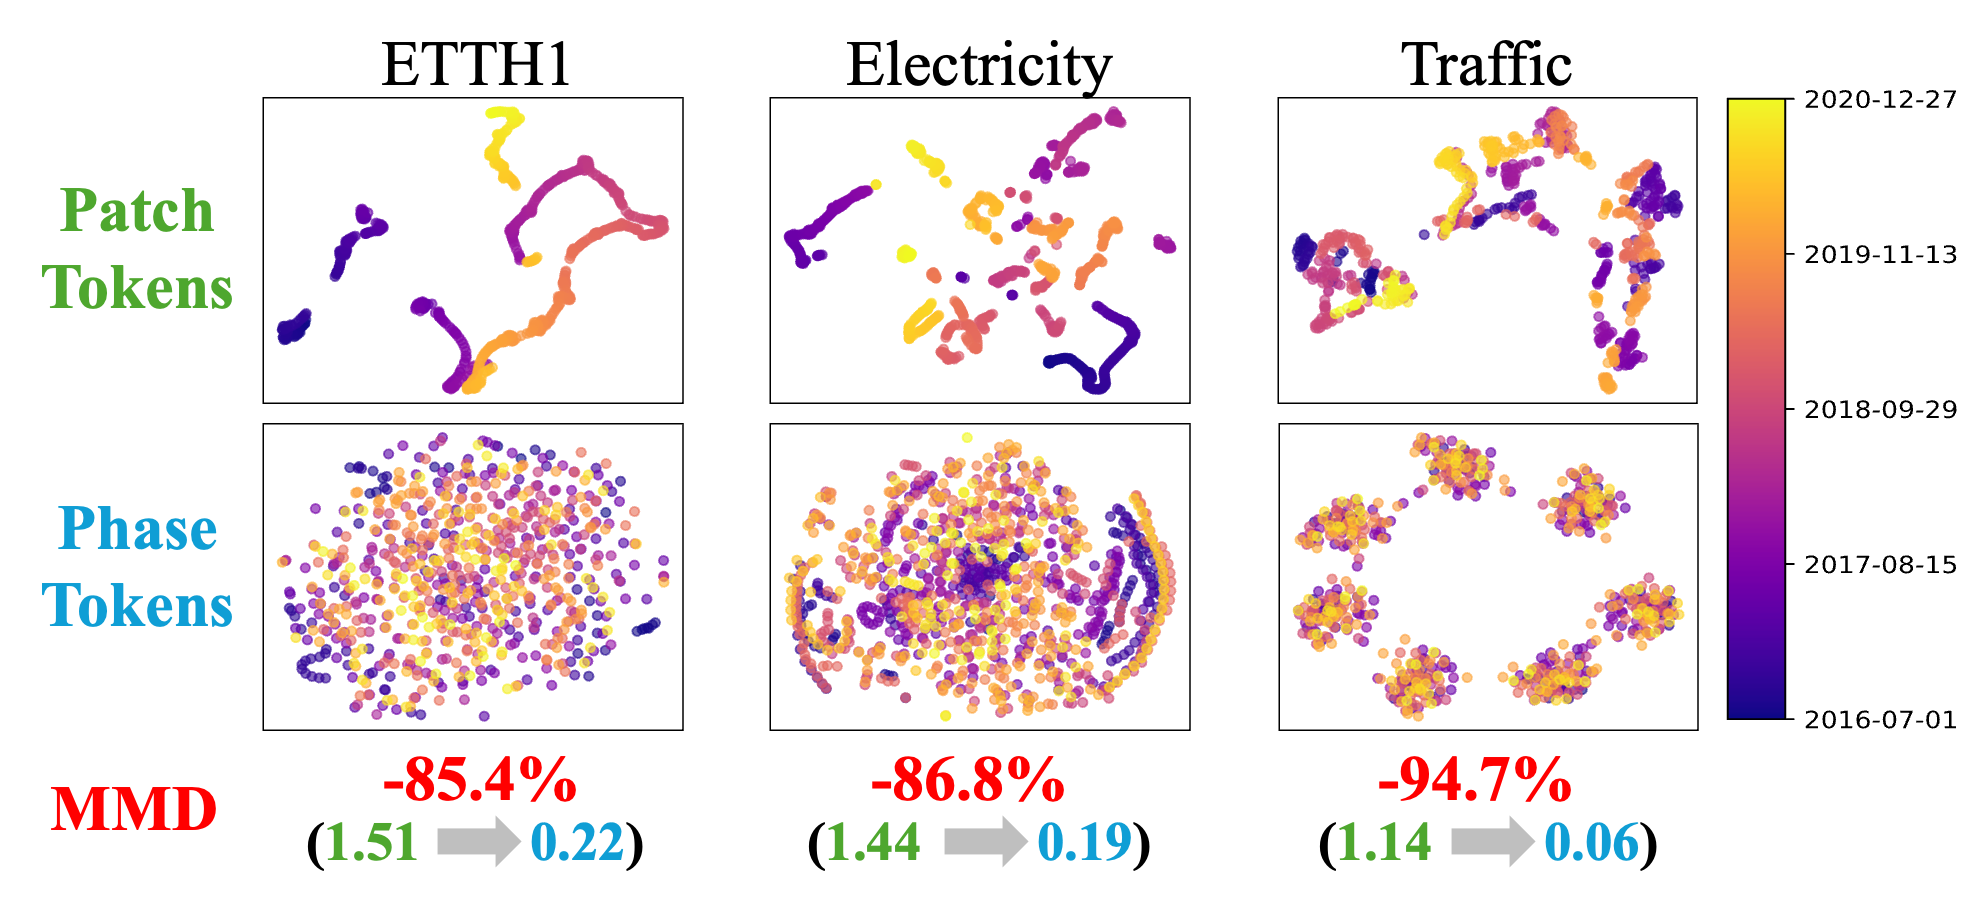
\includegraphics[width=\linewidth]{figures/visualization_cycle_phase_comparison.png}
    \caption{Temporal shift comparison across multiple datasets.}
    \label{fig:visualization_tsne}
  \end{subfigure}
  \hfill
%  subfigure
  \begin{subfigure}[t]{0.37\textwidth}
    \centering
    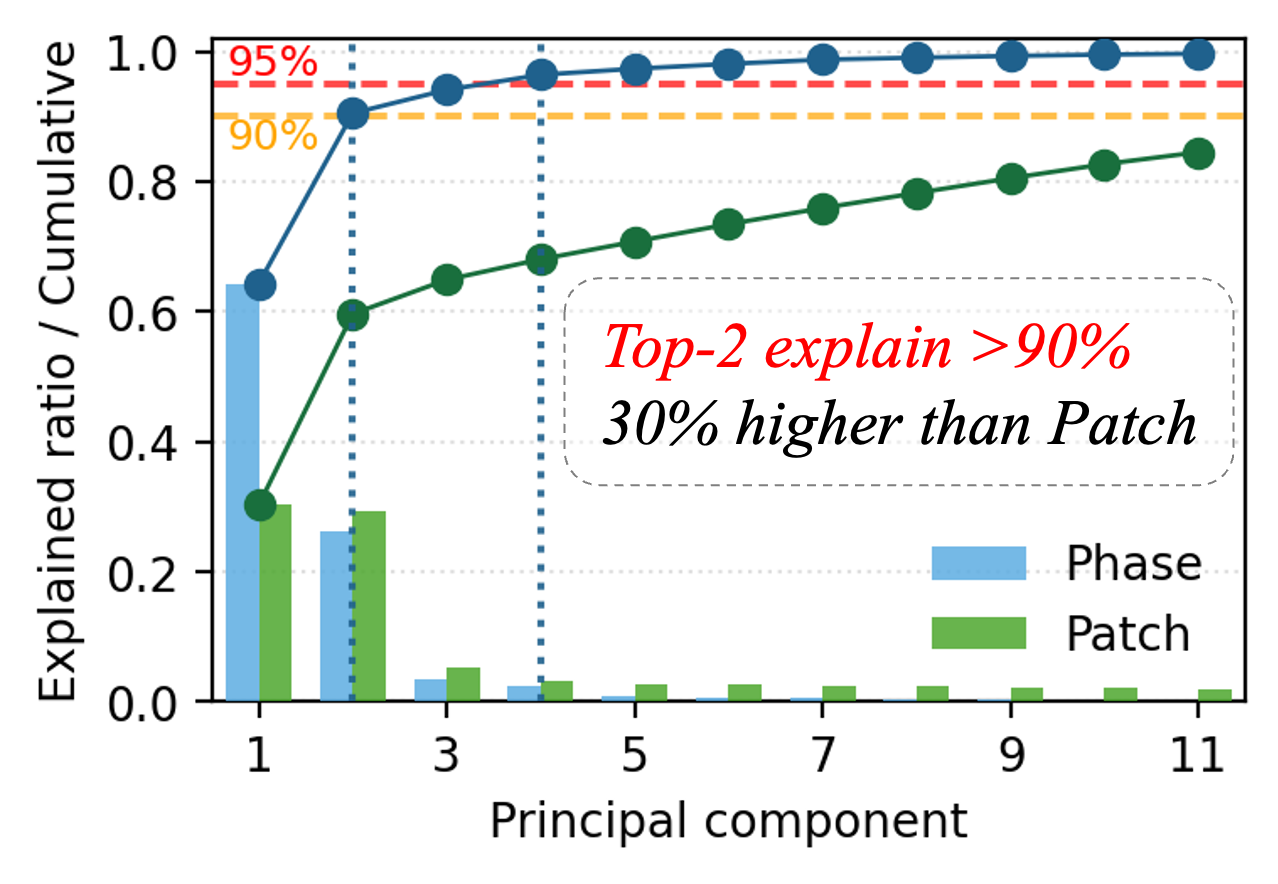
\includegraphics[width=\linewidth]{figures/traffic_pca_cycle_phase.png}
    \caption{PCA for phase tokens on \emph{Traffic}.}
    \label{fig:traffic_pca_cycle_phase}
  \end{subfigure}
  \caption{Visualization of phase tokenization and its advantages.  
  (a) Phase tokenization yields more stable representations than patch-based embeddings.
  (b) Phase tokens exhibit clear low-dimensionality compared with patch tokens.}  
  \label{fig:phase_token_comparison}
\end{figure*}


\subsection{\blue{Phase Tokens Are Stable and Low-Dimensional}}
\label{sec:mot_stability}

To motivate our approach, we conduct a comparative analysis of the geometric structures of patch and phase tokens across three widely used datasets. 
As illustrated in \figref{fig:phase_token}, a patch token is composed of adjacent observations within a local period, whereas a phase token is constructed by extracting values at identical offsets across consecutive periods. We gain the following two important insights from the thorough analysis. 


\fakeparagraph{Insight 1: Phase tokens are globally stationary, while patch tokens are locally stationary}
To provide an intuitive overview of their geometric structures, we project both types of tokens into two-dimensional spaces using t-SNE~\citep{tsne2008}.
As shown in Fig.~\ref{fig:visualization_tsne}, the distributions of patch tokens drift continuously over time but exhibit local coherence, indicating \emph{local stationarity} and supporting the minimal impact of excluding cycle patterns from intensive processing. In contrast, phase tokens form compact and coherent clusters that remain stable over the long term, reflecting strong \emph{global stationarity}. To rigorously quantify the long-term drift, we compute the average discrepancy distance between each subsequent week and the initial week. Specifically, we adopt the Maximum Mean Discrepancy (MMD) metric~\citep{ouyang2021mmd}, a statistical measure of distributional divergence:
\begin{equation}
\begin{aligned}
\mathrm{MMD}^2(P, Q)
&= \mathbb{E}_{x,x' \sim P}[k(x,x')]
+ \mathbb{E}_{y,y' \sim Q}[k(y,y')]\\
&\quad - 2\,\mathbb{E}_{x \sim P, y \sim Q}[k(x,y)],
\end{aligned}
\end{equation}
where \(P\) and \(Q\) denote tokens collected from two different weeks, respectively, and \(k(\cdot,\cdot)\) is the RBF kernel function. As two distributions become closer, their MMD value approaches zero. The results at the bottom of Fig.~\ref{fig:visualization_tsne} show that the average MMD distance of the phase token space is significantly smaller than that of the patch token space. Taken together, both qualitative and quantitative analyses demonstrate that phase tokenization exhibits substantially lower temporal distribution divergence, thereby \emph{facilitating better generalization across the time axis}.

\fakeparagraph{Insight 2: Phase tokens reside in a lower-dimensional subspace than patch tokens}
To measure the effective dimensionality of the token space, we perform principal component analysis (PCA) on it. Surprisingly, as illustrated in Fig.~\ref{fig:traffic_pca_cycle_phase}, two dimensions are already sufficient to explain over 90\% of the variance of phase tokens, whereas patch tokens require more than eleven dimensions to achieve the same degree of explanation, owing to their drifting behavior observed in Fig.~\ref{fig:visualization_tsne}. Consequently, phase information resides in a low-dimensional subspace, \emph{providing a principled basis for parameter- and computation-efficient modeling}.

\revised{
We further establish, using perturbation theory, that phase tokenization remains stable under perturbations of cycle patterns, whereas patch tokenization exhibits structural drift. 
To formalize this result, we represent a univariate periodic sequence as a two-dimensional matrix via delay embedding and analyze the structural properties of this embedded matrix.
}
Due to space limitations, only the core theorem is presented here, while the detailed proof is provided in \blue{the electronic supplement}.
\begin{theorem}[Phase Tokenization Stability]
\label{thm:stability}
Let $X = A G^\top + N \in \mathbb{R}^{D\times H}$ with 
$\operatorname{rank}(A)=\operatorname{rank}(G)=r \ll \min(D,H)$, 
and consider the transformed data
\begin{equation}
X' = X S^\top + R,
\end{equation}
where \blue{$M=AG^\top$ is the signal and $N'=NS^\top$ the transformed noise, so that} $\|N'\|_2 \le \|S\|_2\|N\|_2$, 
$\|R\|_2 \le \varepsilon(\|M\|_F+\|N\|_F)$, 
and let $\delta_{\min} > 0$ denote the minimal spectral separation. 
Then there exists a universal constant $C>0$ such that:
\begin{enumerate}[leftmargin=2em]
\item For phase tokenization and corresponding subspace $\mathcal U_r$, there exists:
\begin{equation}
d\big(\mathcal U_r(X),\mathcal U_r(X')\big)
\;\le\;
C\,\frac{\|N\|_2+\|N'\|_2+\|R\|_2}{\delta_{\min}},
\end{equation}
with exact invariance in the noiseless case $(N=R=0)$.
\item For patch tokenization and corresponding subspace $\mathcal V_r$, there exists:
\begin{equation}
\begin{aligned}
d\big(\mathcal V_r(X),\mathcal V_r(X')\big)
\;\ge\;&
d\big(\mathrm{Col}(G),\mathrm{Col}(S G)\big)\\
&- C\,\frac{\|N\|_2+\|N'\|_2+\|R\|_2}{\delta_{\min}}.
\end{aligned}
\end{equation}
\end{enumerate}
\end{theorem}

\noindent
\textbf{Takeaways.} 
Phase tokenization is structurally invariant under the cycle pattern change $S$ and only subject to perturbations from noise and small day-to-day mismatches. 
In contrast, patch tokenization generally suffers from a non-vanishing structural offset. 
Hence, \emph{phase tokenization is more robust and consistent under cycle pattern drifts}.


\blue{
\subsection{Changes Across Cycles}
\label{sec:mot_changes}

\begin{figure}[t]
\centering
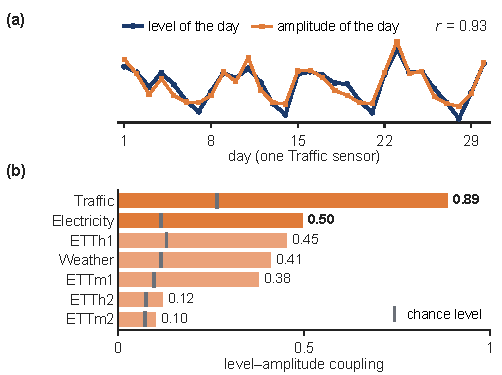
\includegraphics[width=\linewidth]{figures/coupling.pdf}
\caption{Level--amplitude coupling: busier days swing wider. (a)~Thirty days of one Traffic sensor from the test period, a window whose correlation (0.93) is close to the Traffic median; top: hourly occupancy; bottom: the level (mean) and the amplitude (RMS deviation) of each day, standardized. (b)~Sign-consistent coupling over the test windows of every dataset; red ticks: the shifted-pairing reference. A cycle has 24 samples, one day on the hourly datasets.}
\label{fig:coupling}
\end{figure}

\fakeparagraph{What Theorem~\ref{thm:stability} does not cover}
The theorem covers a \emph{common shape change}: $X'=XS^\top$ reshapes every cycle of a window in the same way. Sensor streams also change from one cycle to the next (Fig.~\ref{fig:coupling}(a)). The \emph{level} of a cycle, its mean, moves: a road carries more traffic on some days than on others. The \emph{amplitude} of a cycle, its swing around the level, moves with the level: on a busy day the rush hours rise far above the night, whereas a quiet day stays low and flat. In the folded matrix $X\in\mathbb R^{D\times H}$ of the theorem, with the $D$ cycles as rows and the $H$ phases as columns, these two \emph{changes across cycles} take the form
\begin{equation}
\underbrace{X+\ell\,\mathbf 1^\top}_{\text{level drift}},
\qquad
\underbrace{\operatorname{diag}(\mathbf 1+\alpha\ell)\,X}_{\text{level-dependent amplitude}},
\label{eq:cycle_axis_changes}
\end{equation}
where $\ell\in\mathbb R^D$ holds the cycle levels and $\alpha$ is a coupling strength. Unlike $XS^\top$, which mixes the columns, both act on the rows, so in general neither leaves the span of the phase tokens, $\operatorname{Col}(X)$, unchanged, and Theorem~\ref{thm:stability} no longer applies. With noise, the two changes combine into
\begin{equation}
X_{kp}=\ell_k+(1+\alpha\ell_k)\,s_p+e_{kp},
\qquad
\ell_k=\ell_{k-1}+\eta_k,
\label{eq:mult_model}
\end{equation}
where $X_{kp}$ is the value at phase $p$ of cycle $k$, with a zero-mean seasonal profile $s$, a random-walk level $\ell$ and Gaussian noise. With $\alpha=0$ this is the additive seasonal random-walk model; with $\alpha\neq0$ the swing grows with the level, and we call it the multiplicative seasonal model, after the multiplicative form of Holt--Winters forecasting~\citep{winters1960forecasting}. Under \equref{eq:mult_model}, the phase token of phase $p$ is $s_p\mathbf 1+(1+\alpha s_p)\,\ell$ up to noise: every phase token carries the level, but with a weight that follows the cycle shape, large at the rush hours and small at night. Level-dependent amplitude thus moves the phase tokens specifically, since it multiplies each row, that is, each patch token, by one factor and leaves the span of the patch tokens unchanged.

\fakeparagraph{Insight 3: The within-cycle amplitude moves with the cycle level}
We measure the amplitude of a cycle as its root-mean-square deviation from its mean. In Fig.~\ref{fig:coupling}(a), the levels and amplitudes of the 30 days rise and fall together, with a correlation of 0.93. We compute this correlation for every channel and every window of 720 samples (30 cycles of 24, stride 24), directly on the data. Over 30 cycles, two series that drift independently also correlate by chance, with either sign. We therefore average the correlation over the windows of each channel, keeping its sign, and report the mean magnitude of these channel averages, the \emph{sign-consistent coupling}: chance correlations cancel in the average, a coupling of stable sign does not. As a reference, the same statistic is computed after pairing the levels of every window with the amplitudes of the window half the period away, which keeps the drift of both but removes their alignment.

Fig.~\ref{fig:coupling}(b) shows that five benchmarks lie far above this reference and that the coupling is strongest on the two sensor networks: Electricity, with 321 meters, reaches 0.50, and Traffic, with 862 road sensors, 0.89. On these two networks the correlation is positive in 84\% and in over 99\% of the windows, respectively, so a busier day swings wider. Weekends do not explain this: over the weekday cycles of each window alone, the coupling is still 0.51 and 0.82. On ETTh1 and ETTm1, the sign differs between channels but is stable within each, so the amplitude grows with the level on some channels and shrinks on others. ETTh2 and ETTm2 show the weakest coupling, little above the reference. On the training and validation periods, too, the two sensor networks are the most and ETTh2 and ETTm2 the least coupled (electronic supplement). Hence, \emph{wherever its sign is stable, a phase-token model must produce a cycle shape that scales with the level}.

This coupling within a window does not contradict Insight~1, which compares the distribution of phase tokens across weeks. Section~\ref{sec:extension} adds one component to \sysname for each of the two changes, and Section~\ref{sec:theory} shows why each takes its form and that the coupling forces an error floor only where it drives the amplitude beyond an envelope that the trained weights fix, which Section~\ref{sec:exp_envelopes} measures.
}


\section{Methodology}
\label{sec:method}

Given the focus on periodicity, we adopt the channel-independent paradigm~\citep{nie2023patchtst, zeng2023dlinear} and omit the channel dimension throughout the remainder of this paper\blue{; the $C$ channels of a dataset share one model}. The objective of forecasting is to predict the future trajectory $\mathbf{Y}\in\mathbb{R}^{L_{\text{out}}}$ from an input sequence $\mathbf{X}\in\mathbb{R}^{L_{\text{in}}}$, where $L_{\text{in}}$ and $L_{\text{out}}$ denote the input and output lengths, respectively. In the following sections, we describe the data preprocessing procedure, present the proposed network architecture \blue{and the scope of its phase alignment, introduce its level--amplitude extension, and finally analyze the computational complexity of both}.

\begin{figure*}[t]
    \centering
    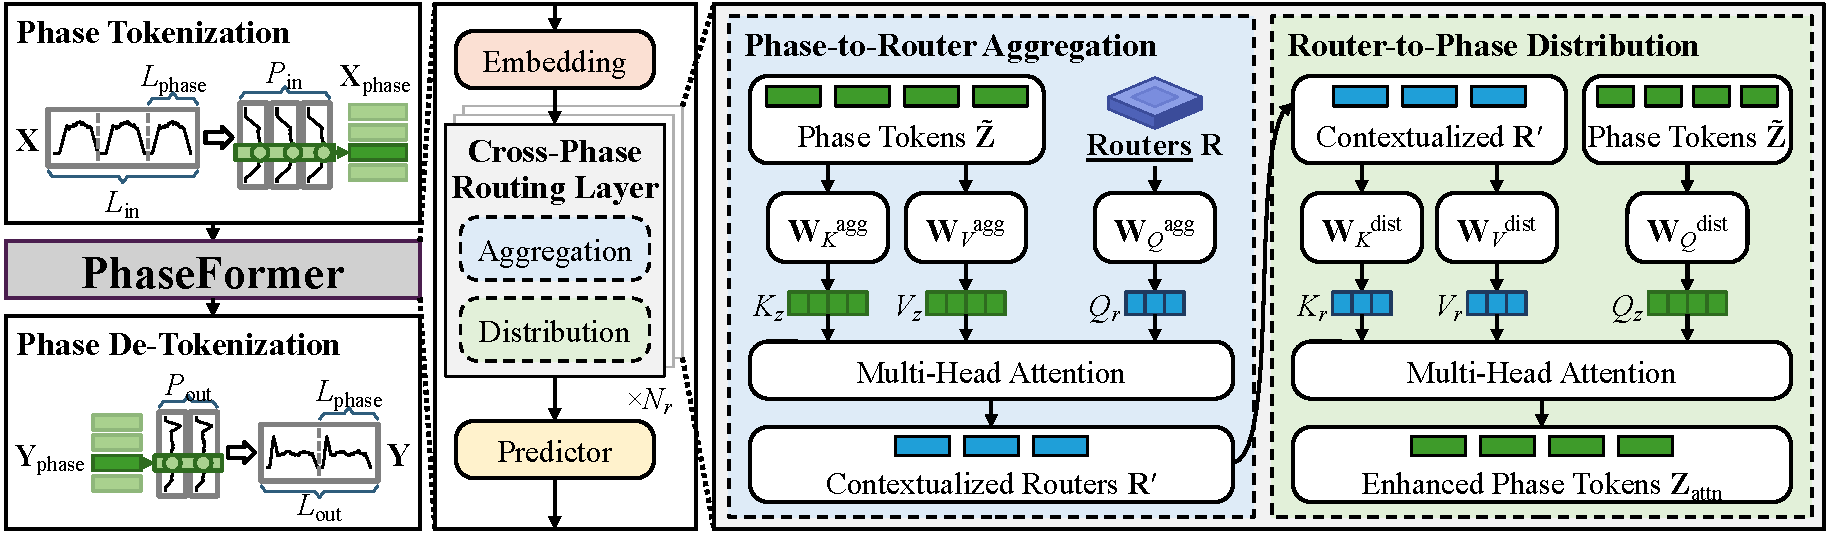
\includegraphics[width=\textwidth]{figures/phaseformer_overview.pdf}
    \caption{\blue{Overview} of \sysname.}
    \label{fig:overview}
\end{figure*}

\subsection{Data \blue{Preprocessing}}
\label{subsec:phase-embedding}
\fakeparagraph{Normalization and De-Normalization}
Following \cite{kim2021reversible}, we normalize inputs with their estimated mean and standard deviation, and de-normalize predictions to the original scale. \blue{This normalization (RevIN) maps an input window $x$ with mean $\mu$ and standard deviation $\sigma$ to $\tilde x=(x-\mu\one)/\sigma$, so that $\one^\top\tilde x=0$, and a forecast $\hat{\tilde y}$ in these coordinates is de-normalized to $\hat y=\mu\one+\sigma\hat{\tilde y}$.}

\fakeparagraph{Phase Tokenization and De-Tokenization}
Phase tokenization transforms the one-dimensional input sequence into a two-dimensional phase--period matrix for \blue{subsequent} processing.
Conversely, phase de-tokenization reconstructs the predicted phase--period matrix back into a one-dimensional output sequence.
\revised{\blue{Let $L_{\text{phase}}$ denote the period length; it is estimated by frequency analysis (\secref{sec:phase_length}) and kept fixed.}}

To ensure that the input sequence length is a multiple of $L_{\text{phase}}$, we circularly pad the sequence to length \blue{$P_{\text{in}}L_{\text{phase}}$}, where $P_{\text{in}} = \left\lceil \frac{L_{\text{in}}}{L_{\text{phase}}} \right\rceil.$
As illustrated in \figref{fig:overview}, the padded sequence $\mathbf{X}$ is then reshaped into a phase--period matrix $\mathbf{X}_{\text{phase}} \in \mathbb{R}^{L_{\text{phase}} \times P_{\text{in}}}$, where each entry \blue{$\mathbf{X}_{\text{phase}}[p, k]$ corresponds to the observation at the $p$-th phase of the $k$-th cycle}.
\blue{De-tokenization reverses this reshaping.}

\blue{
\fakeparagraph{Notation}
We abbreviate $P=\Lp$ for the period, $K=\Pin$ and $K'=\Pout$ for the numbers of input and output cycles, $L=KP$ and $H=K'P$. In all \sysLA experiments $L=720$, $P=24$ and $K=30$, and every horizon $H\in\{96,192,336,720\}$ is a whole number of cycles, so that no padding occurs. The folded normalized window $\tilde X\in\mathbb R^{K\times P}$, the transpose of the phase--period matrix of $\tilde x$, has one row per cycle as in Section~\ref{sec:mot_changes}; its columns are the phase tokens $\tilde x_p\in\mathbb R^K$, and its row means are the cycle means $\bar r=\tfrac1P\tilde X\one_P\in\mathbb R^K$.
}

% --------------------------------------------------------------------
\subsection{Phase-\blue{Based} Routing Transformer}
\label{subsec:phase-network}

The phase--period matrix is fed into our proposed phase-based routing Transformer, termed \sysname, to capture and extrapolate temporal dynamics at the phase level.
As illustrated in \figref{fig:overview}, \sysname first applies an embedding layer to the phase tokens, then refines them through multiple cross-phase routing layers, and finally maps them to the target via a shared predictor.

% ---------------- embedding ----------------
\subsubsection{Embedding Layer}
\label{subsubsec:phase-embedding}
The embedding layer projects the phase tokens $\mathbf{X}_{\text{phase}}$ into a low-dimensional representation space, allowing the informative components to be extracted from raw observations that are often contaminated by perturbations.
Formally, for each phase index \blue{$p \in \{1,\dots,L_{\text{phase}}\}$, the corresponding phase token $\mathbf{X}_{\text{phase}}[p, :]$} is mapped into a $d$-dimensional representation through \blue{an affine map $f_{\theta}$ with weight $W_e\in\mathbb R^{d\times\Pin}$ and bias $c_e\in\mathbb R^d$, followed by a LayerNorm $\LN_e$~\citep{ba2016layernorm}}:
\begin{equation}
\mathbf{Z}
= \blue{\LN_e\big(}f_{\theta}\!\left(\mathbf{X}_{\text{phase}}\right)\blue{\big)}\in \mathbb{R}^{L_{\text{phase}}\times d}
\label{eq:phase-embedding}
\end{equation}

To better capture the temporal ordering among phases, we introduce a set of learnable positional embeddings $\mathbf{E}_{\text{pos}}\in\mathbb{R}^{L_{\text{phase}}\times d}$ \blue{to encode the position of each phase within the cycle}, following \cite{liu2023spatio}.
These embeddings are added to $\mathbf{Z}$ in a phase-wise manner, so that each phase representation is enriched with its positional information:
\begin{equation}
\tilde{\mathbf{Z}}=\mathbf{Z}+\mathbf{E}_{\text{pos}}.
\end{equation}
The resulting $\tilde{\mathbf{Z}}$ is then forwarded to the cross-phase routing layers for higher-level feature interaction and forecasting\blue{; in a stack of layers, every layer adds its own positional embeddings to its input in this way}.

% ---------------- Attention ----------------
\subsubsection{Cross-Phase Routing Layer}

Directly modeling full pairwise interactions among phase representations via self-attention is computationally expensive.
To handle this, we introduce a set of learnable routers $\mathbf{R}\in\mathbb{R}^{M\times d}$ to mediate information exchange across phases.
\revised{
While the design is inspired by prior routing-style \blue{designs}~\citep{jaegle2021perceiver, zhang2023crossformer}, our contribution lies in \emph{leveraging the inherent low-rank structure of phase-aligned tokens} \blue{(Insight~2, Section~\ref{sec:mot_stability})}.
\blue{Cross-phase routing reduces the quadratic cost of self-attention to a cost linear in the number of phases, while every phase can still exchange information with every other phase.}
}

Cross-phase routing consists of two steps:
(i) \emph{phase-to-router aggregation}, which selectively compresses information from phase representations into the compact set of routers; and (ii) \emph{router-to-phase distribution}, which selectively propagates the aggregated cross-phase information from the routers back to the phase representations. Both steps are implemented via cross-attention.

\fakeparagraph{Phase-to-Router Aggregation}
The routers attend to the phase representations to extract contextual information, yielding contextualized router embeddings
\blue{$\mathbf{R}'\in\mathbb{R}^{M\times d}$}.
Specifically, the routers act as queries while the phases provide keys and values. The projection matrices
$\mathbf{W}_Q^{\text{agg}},\mathbf{W}_K^{\text{agg}},\mathbf{W}_V^{\text{agg}}\in\mathbb{R}^{d\times d}$
map the representations into query, key, and value spaces, respectively:
\begin{equation}
\mathbf{Q}_r=\mathbf{R}\mathbf{W}_Q^{\text{agg}},\quad
\mathbf{K}_z=\tilde{\mathbf{Z}}\mathbf{W}_K^{\text{agg}},\quad
\mathbf{V}_z=\tilde{\mathbf{Z}}\mathbf{W}_V^{\text{agg}}.
\end{equation}
The aggregated router embeddings are then obtained via multi-head attention (MHA) with \blue{$n_h$} heads:
\begin{equation}
\blue{\mathbf{R}'}=\mathrm{MHA}\!\left(\mathbf{Q}_r,\mathbf{K}_z,\mathbf{V}_z\right).
\end{equation}

\fakeparagraph{Router-to-Phase Distribution}
The aggregated information in the routers is subsequently redistributed to the phase representations, thereby enabling cross-phase information flow. In this step, the phase representations serve as queries while the routers provide keys and values, yielding refined phase representations $\mathbf{Z}_{\text{attn}}$. The projection matrices $\mathbf{W}_Q^{\text{dist}}, \mathbf{W}_K^{\text{dist}}, \mathbf{W}_V^{\text{dist}}\in\mathbb{R}^{d\times d}$ are used for this distribution:
\begin{equation}
\mathbf{Q}_z=\tilde{\mathbf{Z}}\mathbf{W}_Q^{\text{dist}},\quad
\mathbf{K}_r=\blue{\mathbf{R}'}\mathbf{W}_K^{\text{dist}},\quad
\mathbf{V}_r=\blue{\mathbf{R}'}\mathbf{W}_V^{\text{dist}},
\end{equation}
\begin{equation}
\mathbf{Z}_{\text{attn}}=\mathrm{MHA}\!\left(\mathbf{Q}_z,\mathbf{K}_r,\mathbf{V}_r\right).
\end{equation}
This mechanism restores phase-level resolution while simultaneously enforcing coherence across phases through the contextualized routers.
Ultimately, each phase representation attends to all others through a two-stage routing pathway.
\blue{The two steps are wrapped in residual connections, two LayerNorms and an MLP: writing $z_p$ and $m_p$ for the $p$-th rows of the layer input ($\tilde{\mathbf Z}$ for the first layer) and of $\mathbf Z_{\text{attn}}$, a routing layer outputs $o_p=\LN_1(z_p+m_p)$ and $h_p=\LN_2\big(o_p+\mathrm{MLP}(o_p)\big)$. Each LayerNorm centers its input over the $d$ features, rescales it to unit root mean square, and applies a learned gain $\gamma_i$ and offset $\beta_i$: $\LN_i(u)=\gamma_i\odot\varsigma+\beta_i$ with $\varsigma=J_du/(\|J_du\|^2/d+\epsilon)^{1/2}$ and $J_d=I_d-\tfrac1d\one\one^\top$. Hence $\|\varsigma\|<\sqrt d$ for every input, and every latent $h_p$ of the last layer is an output of its $\LN_2$; Section~\ref{sec:theory} builds on these two facts. Appendix~\ref{app:proofs} states the full layer.}


% ---------------- predictor ----------------
\subsubsection{Predictor}
\label{subsubsec:phase-predictor}

The predictor produces multi-step forecasts of length $P_{\text{out}}$ for all phases simultaneously, based on their refined representations. Taking as input the \blue{final phase latents $\mathbf Z_{\text{out}}=[h_1;\dots;h_{L_{\text{phase}}}]\in\mathbb{R}^{L_{\text{phase}}\times d}$ of the last} cross-phase routing layer, the predictor is realized as \blue{an affine} mapping \blue{$g_{\Phi}$}, parameterized by \blue{a weight $\Phi\in\mathbb{R}^{P_{\text{out}}\times d}$ and a bias $c_\Phi\in\mathbb{R}^{P_{\text{out}}}$ and applied to every phase}:
\begin{equation}
\begin{gathered}
\mathbf{Y}_{\text{phase}} = \blue{g_{\Phi}(\mathbf Z_{\text{out}})}
\in \mathbb{R}^{L_{\text{phase}}\times P_{\text{out}}}\blue{,}\\
\blue{F_p=\Phi h_p+c_\Phi\in\mathbb R^{K'}.}
\end{gathered}
\label{eq:predictor}
\end{equation}
\blue{The $p$-th row of $\mathbf Y_{\text{phase}}$ holds the $K'$ future values $F_p$ of phase $p$ in normalized units. Unfolding the phases cycle by cycle gives the \emph{phase forecast} $F\in\mathbb R^H$, and we call the computation from the phase tokens to $F$ the \emph{phase path}; for \sysname, the forecast is $\hat{\tilde y}=F$.}
All phases share the same predictor parameters, which enforces consistency across phases and reduces the number of trainable parameters. This not only improves efficiency but also regularizes learning, thereby enhancing generalization. Finally, the predicted phase--period matrix $\mathbf{Y}_{\text{phase}}$ is passed through de-tokenization and de-normalization to produce the final forecast $\mathbf{Y}$.


\revised{
\subsection{\blue{Scope of Phase Alignment}}
\label{sec:discussion}

\blue{
\fakeparagraph{Weak Periodicity}
Although \sysname is built around periodic alignment, it remains usable on weakly periodic or partially non-periodic time series. When no strong periodic structure is present, the phase representation degenerates into a coarse subsampling of the sequence: the phase tokens resemble trend embeddings sampled every $\Lp$ steps and capture slowly varying components and broad temporal structure. Through the routing mechanism, the model can still aggregate information across these coarse tokens, which suppresses high-frequency noise, prevents overfitting to short-term stochastic fluctuations, and retains a certain degree of robustness without a clear period.

\fakeparagraph{Failure Modes}
In datasets without a clear dominant period, the estimated phase length may be affected by noise or minor harmonics, and the resulting misalignment is the primary failure mode of the model. In multi-period settings, a model aligned to a suboptimal harmonic instead of the dominant component still operates but delivers inferior forecasts (\secref{sec:phase_length}). A phase length that is excessively large or small also introduces substantial circular padding, which injects artificial boundary information and degrades the forecasts; input lengths divisible by the phase length avoid it and are recommended whenever possible.

This subsection concerns series without a reliable period. Within a periodic series, the changes across cycles of Section~\ref{sec:mot_changes} are a different limitation, which the extension below addresses.
}
}


\blue{
\subsection{\sysLA: Supplying the Missing Level and Amplitude}
\label{sec:extension}

\sysname was not designed for the changes across cycles of Section~\ref{sec:mot_changes}. A trained \sysname follows them only within two envelopes fixed by its final LayerNorm and its predictor, one for the level and one for the within-cycle amplitude, and Section~\ref{sec:theory} shows that what lies outside them has a simple form (Table~\ref{tab:two_envelopes}). \sysLA supplies this remainder with two components and keeps the backbone unchanged: phase tokenization, embedding, cross-phase routing and the shared predictor are those of \sysname. A level branch with a gated fusion addresses level drift; we call \sysname with these two parts \sysL. A centered modulation of the final phase latents addresses level-dependent amplitude; adding it to \sysL gives \sysLA. Fig.~\ref{fig:la_overview} shows where the components attach.

\begin{figure*}[t]
\centering
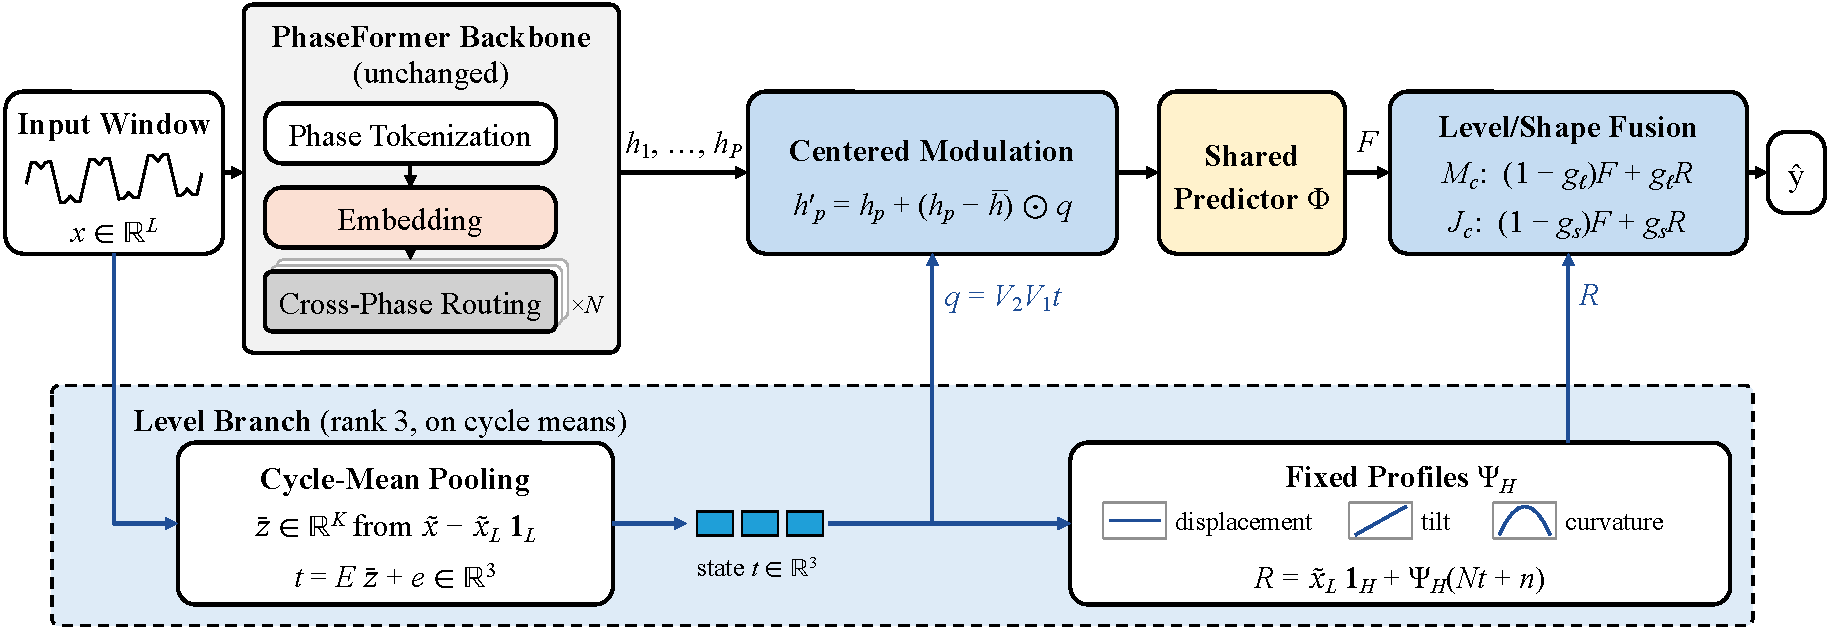
\includegraphics[width=\textwidth]{figures/la_overview.pdf}
\caption{\sysLA. The \sysname backbone and the shared predictor are unchanged and keep the colors of Fig.~\ref{fig:overview}; the new components are blue. A rank-3 level branch reads the anchored cycle means and writes onto three fixed horizon profiles; its state $t$ drives a centered modulation of the final phase latents; the two forecasts are fused with separate level and shape gates.}
\label{fig:la_overview}
\end{figure*}

\fakeparagraph{Notation}
In addition to the notation of Section~\ref{subsec:phase-embedding}, let $\tilde x_L$ be the last value of the normalized window. Let $M_c$ be the orthogonal projection of $\mathbb R^H$ onto the vectors that are constant within each future cycle, and $J_c=I-M_c$: $M_c$ replaces every future cycle by its mean, the level of that cycle, and $J_c$ keeps the deviations within each cycle, its shape. Finally, $\lev(v)=\tfrac1H\one^\top v$ is the level of a forecast $v\in\mathbb R^H$.

\subsubsection{Level Branch and Gated Fusion}
\label{sec:ext_branch}

Level drift adds the same vector of cycle levels to every phase token~\equref{eq:cycle_axis_changes}, so the level of a window is carried by its cycle means, and the level of the future is smooth over the horizon. The branch therefore reads only the cycle means and writes onto a few smooth profiles (left of Fig.~\ref{fig:la_overview}). It pools the anchored window $\tilde x-\tilde x_L\one_L$ to its cycle means $\bar r-\tilde x_L\one_K$ and maps them to a rank-3 state,
\begin{equation}
\begin{gathered}
t=E(\bar r-\tilde x_L\one_K)+c_E\in\mathbb R^3,\\
F_{\mathrm b}=\tilde x_L\one_H+\Psi_H\,(\Gamma t+c_\Gamma),
\end{gathered}
\label{eq:branch}
\end{equation}
where $\Psi_H=[\one_H,a_2,a_3]\in\mathbb R^{H\times3}$ holds the displacement, tilt and curvature profiles, the discrete orthogonal polynomials of degree $0,1,2$ on the forecast grid, normalized to unit root mean square, so that its first column is $\one_H$ and the other two are horizon-centered. $\Psi_H$ is fixed; only $E\in\mathbb R^{3\times K}$, $c_E\in\mathbb R^3$, $\Gamma\in\mathbb R^{3\times3}$ and $c_\Gamma\in\mathbb R^3$ are learned. Theorem~\ref{thm:complement} explains why a map of low rank onto fixed profiles is enough; the main-table configuration replaces $\Psi_H$ by a learned decoder of the same rank on four settings (Appendix~\ref{app:la_config}). The anchor makes the branch shift-equivariant in normalized coordinates: adding $c\one_L$ to $\tilde x$ leaves $t$ unchanged and adds $c\one_H$ to $F_{\mathrm b}$. The branch reads the window directly and is fused after the shared predictor, so, unlike the phase forecast, it passes through no LayerNorm of the backbone; Section~\ref{sec:theory_level} shows why this matters.

\fakeparagraph{Gated Fusion}
For every future cycle, the fused forecast takes its level and its within-cycle shape from $F$ and $F_{\mathrm b}$ with separate gates,
\begin{equation}
\begin{gathered}
M_c\hat{\tilde y}=(1-g_\ell)M_cF+g_\ell M_cF_{\mathrm b},\\
J_c\hat{\tilde y}=(1-g_s)J_cF+g_sJ_cF_{\mathrm b},
\end{gathered}
\label{eq:fusion}
\end{equation}
with $g_\ell=\operatorname{sigmoid}(\omega)$ and $g_s=\operatorname{sigmoid}(\omega+\delta)$. Since $J_c\one_H=0$, the branch enters the within-cycle shape only through the within-cycle parts $J_ca_2$ and $J_ca_3$ of its tilt and curvature profiles. The gates are static: they depend on neither the input nor the time step. They are learned either per channel or shared across the $C$ channels, a choice made per dataset in the protocol configuration and per setting in the main-table configuration (Section~\ref{sec:ext_setup} and Appendix~\ref{app:la_config}).

\subsubsection{Centered Amplitude Modulation}
\label{sec:ext_modulation}

Level-dependent amplitude scales the cycle shape with the level. Before the shared predictor, \sysLA scales the deviations of the final phase latents $h_1,\dots,h_P$ from their mean over the phases, elementwise, by a vector $q$ computed from the branch state $t$, which carries the level forecast (center of Fig.~\ref{fig:la_overview}):
\begin{equation}
h'_p=h_p+(h_p-\bar h)\odot q,\qquad \bar h=\tfrac1P\textstyle\sum_ph_p,\qquad q=V_2V_1\,t,
\label{eq:la_modulation}
\end{equation}
with $V_1\in\mathbb R^{k_q\times3}$, $V_2\in\mathbb R^{d\times k_q}$, $k_q=\min(w,3,d)$ and no biases; the width $w$ is $2$ by default, and the branch rank caps $k_q$ at $3$. The predictor then receives $h'_p$ in place of $h_p$. Because the predictor~\equref{eq:predictor} is shared and affine, $\Phi\bar h+c_\Phi$ is the vector of future cycle means of the phase forecast: $\bar h$ is the latent counterpart of the cycle level, and $h_p-\bar h$ that of the within-cycle shape. The deviations sum to zero over the phases, so the modulation leaves every future cycle mean of the phase forecast unchanged (Proposition~\ref{prop:modulation}(a)): it changes only the within-cycle part of the phase forecast, never its cycle means, and $q=q_1\one_d$ scales that part by $1+q_1$. This centering is over the phases, not over the features as in a LayerNorm.

\subsubsection{Nesting and Initialization}
\label{sec:ext_properties}

The new parameters are initialized so that the components start from simple forecasts. $\Gamma$ and $c_\Gamma$ are zero, so the branch initially forecasts the last value; $V_2$ is zero, so the modulation is initially the identity; and both gates start at a common value $g_0$ ($\delta=0$), $0.2$ by default. With $V_2=0$, \sysLA reduces exactly to \sysL, and \sysL tends to \sysname as $g_\ell,g_s\to0$. Hence \sysLA and \sysL built from the same random state with the same gate initialization have identical forecasts at initialization, which our experiments use to pair them. We write \sysLA (mod.\ off) for a trained \sysLA evaluated with $V_2=0$.
}

\subsection{Complexity of \sysname{} \blue{and \sysLA}}
\label{sec:complexity}

For each \blue{channel}, the overall complexity of \sysname\ can be summarized as follows:
the phase embedding layer requires $O(L_{\text{phase}} P_{\text{in}} d)$ time and $O(L_{\text{phase}} d)$ memory.
The cross-phase routing layer, which dominates computation, incurs $O((L_{\text{phase}}+M)d^2 + M L_{\text{phase}} d)$ time and $O(\blue{n_h} M L_{\text{phase}} + (L_{\text{phase}}+M)d)$ memory.
Finally, the predictor costs $O(L_{\text{phase}} d P_{\text{out}})$ time and $O(L_{\text{phase}} P_{\text{out}})$ memory.
Aggregating across \(\blue{N_r}\) \blue{routing layers and substituting} $P_{\text{in}}=\lceil L_{\text{in}}/L_{\text{phase}}\rceil$ and
$P_{\text{out}}=\lceil L_{\text{out}}/L_{\text{phase}}\rceil$\blue{, the end-to-end time complexity is}
\[
O\Big(\blue{N_r}\big((L_{\text{phase}}+M)d^2 + M L_{\text{phase}} d\big)
+ d(L_{\text{in}}+L_{\text{out}})\Big).
\]
As investigated in \secref{sec:mot_stability}, the phase token space exhibits \blue{an} inherently low-dimensional structure, which allows $M$ and $d$ to be chosen as fixed and small numbers.
Thus, \blue{for a fixed number of layers,} the computational cost grows \blue{linearly} with both the input length $L_{\text{in}}$ and the output horizon $L_{\text{out}}$.

\blue{
\fakeparagraph{Cost of \sysLA}
The level branch adds $3K$ ($E$) $+\,3$ ($c_E$) $+\,9$ ($\Gamma$) $+\,3$ ($c_\Gamma$) $=105$ parameters at $K=30$ with the fixed profiles of \equref{eq:branch}, the modulation $k_q(3+d)$, and the gates $2C$ for $C$ channels, or two in total when shared; none of these depends on the forecast horizon. The branch costs $O(L)$ per channel for pooling and $O(K+H)$ for the readout, and the modulation $O(Pd)$, against the $O\big(N_r((P+M)d^2+MPd)+d(L+H)\big)$ of \sysname, so the overall complexity remains linear in the input and output lengths and in the number of channels.
}

\blue{
\section{How Far \sysname Can Follow Changes Across Cycles}
\label{sec:theory}

Section~\ref{sec:mot_changes} identified two changes across cycles that Theorem~\ref{thm:stability} does not cover, level drift and level-dependent amplitude, and Section~\ref{sec:extension} added two components for them. This section explains why the components take this form. For level drift we answer three questions in turn: can \sysname represent the change at all, how far can a trained model follow it, and what is the simplest component that carries the remainder (Section~\ref{sec:theory_level}). For level-dependent amplitude we answer the last two (Section~\ref{sec:theory_amplitude}). Section~\ref{sec:theory_design} maps the results to the design of \sysLA. We use the notation of Section~\ref{sec:extension}; proofs are in Appendix~\ref{app:proofs}.

\subsection{Error Decomposition}
\label{sec:theory_setup}

Every routing unit of \sysname ends with a LayerNorm $\LN_2$ (Section~\ref{subsec:phase-network}), which maps $u\in\mathbb R^d$ to $\gamma\odot\varsigma+\beta$ with $\varsigma=J_du/(\|J_du\|^2/d+\epsilon)^{1/2}$ and $J_d=I_d-\tfrac1d\one\one^\top$~\citep{ba2016layernorm}. The shared predictor~\equref{eq:predictor} reads the output of the last unit.

Let $\tilde y=(y-\mu\one)/\sigma$ be the future in the window's coordinates. Any error $e=\hat{\tilde y}-\tilde y$ splits orthogonally into a level part, a cycle-to-cycle part and a within-cycle part:
\begin{equation}
\tfrac1H\|e\|^2=\lev(e)^2+\tfrac1H\|J_HM_ce\|^2+\tfrac1H\|J_ce\|^2 .
\label{eq:error_split}
\end{equation}
The first term is governed by the \emph{level demand} of a window, $\Lambda=\lev(\tilde y)=(m_y-\mu)/\sigma$, the distance of the future mean from the window mean in units of the window's standard deviation. The last term is governed by the shape of the future cycles, and Section~\ref{sec:theory_amplitude} introduces the corresponding \emph{amplitude demand}.

The stylized model behind the analysis is the multiplicative seasonal model~\equref{eq:mult_model} of Section~\ref{sec:mot_changes}, in which $X_{kp}$ is the value at phase $p$ of cycle $k$ and $s\in\mathbb R^P$ is the seasonal profile.

\subsection{Level Drift}
\label{sec:theory_level}

With $\alpha=0$, model~\equref{eq:mult_model} is the additive seasonal random-walk model, for which the Bayes forecast of every future cycle is a recency-weighted average $b^\top\bar r$ of the cycle means added to each phase's long-run value, with Kalman weights $b$ (Lemma~\ref{lem:bayes}). In folded coordinates a level trajectory adds the \emph{same} vector to every phase token, and this common-shift structure drives the level results.

\fakeparagraph{Capability}
The first result shows that the architecture can represent level drift, and how.
\begin{theorem}[Structural level capability]
\label{thm:capability}
Consider \sysname with one routing layer, latent width $d\ge4$, any number of routers and heads.
(a) It is exactly equivariant to the window's level and scale: $F(a x+c\one)=aF(x)+c\one$ for $a>0$.
(b) A cycle-level trajectory enters every phase token as a common shift, and router attention transmits a common shift exactly: sender weights are unchanged and every router buffer shifts by the same vector.
(c) For every weight vector $b$ with $\one^\top b=1$ and $\|b\|\le1$, there are parameters $\theta_c$, $c^2\ge5L$, whose forecast approximates the level-adaptive seasonal forecaster $G_b$ uniformly over all normalized windows, with error at most $\kappa L^{3/2}/c^2$ for an absolute constant $\kappa$. In particular, \sysname can approximate the Bayes forecast of model~\equref{eq:mult_model} with $\alpha=0$ to any accuracy.
\end{theorem}

The construction makes the LayerNorms transparent by a large offset $c$ along one latent direction and uses two further directions to carry the phase's long-run value and the recency-weighted level. The offset is not free: the next theorem shows that it is exactly the size of the model's level envelope.

\fakeparagraph{Level envelope}
Let $A=\Phi\operatorname{diag}(\gamma_2)$ and $o=\Phi\beta_2+c_\Phi$ be read from the last unit, and define
\begin{equation}
\begin{gathered}
c_0=\tfrac{1}{K'}\one^\top o,\quad
C_1=\tfrac{\sqrt d}{K'}\big\|J_dA^\top\one_{K'}\big\|,\\
\mathcal I_\varphi=(c_0-C_1,\,c_0+C_1),
\end{gathered}
\label{eq:envelope_constants}
\end{equation}
and $C_\varphi=|c_0|+C_1$.

\begin{theorem}[Level envelope]
\label{thm:level_envelope}
For every parameter value of \sysname (any depth, routers, heads, positional embeddings and MLP weights) and every input window:
(a) every normalized phase forecast lies in the fixed ellipsoid $\mathcal E_\theta=\{o+A\varsigma:\ \varsigma\perp\one_d,\ \|\varsigma\|<\sqrt d\}$;
(b) the forecast level lies in the envelope, $\lev(\hat{\tilde y})\in\mathcal I_\varphi$, so that $|m_{\hat y}-\mu|<C_\varphi\sigma$ in original units;
(c) for every window with level demand $\Lambda$,
\begin{equation}
\tfrac1H\|\hat y-y\|^2\ \ge\ \sigma^2\operatorname{dist}(\Lambda,\mathcal I_\varphi)^2\ \ge\ \sigma^2(|\Lambda|-C_\varphi)_+^2 ;
\label{eq:level_floor}
\end{equation}
(d) the level and the shape of a phase compete for the same budget: as the level of phase $p$ approaches the boundary of $\mathcal I_\varphi$, the input-dependent part of its forecast is forced onto the single profile $AJ_dA^\top\one$.
\end{theorem}

The theorem uses nothing about routing, attention or depth: those components decide which point of $\mathcal E_\theta$ is produced, never the set itself, and the constants are read directly from a checkpoint. Because RevIN makes the demand dimensionless, the envelope binds on windows whose level departure is large relative to their own variation, whatever its absolute size.

\begin{corollary}[Steps and trends]
\label{cor:steps}
A persistent step that occurred $m$ samples before the forecast origin has level demand tending to $\sqrt{(L-m)/m}$ as the step grows relative to the background, and a linear trend that continues through the horizon has $\Lambda=\sqrt3(L+H)/\sqrt{L^2-1}$. Any step more recent than $L/(1+C_\varphi^2)$ samples therefore demands a level outside every envelope of half-width $C_\varphi$, and at $L=720$ a continued trend demands $\Lambda=1.96$ to $3.46$ for $H=96$ to $720$.
\end{corollary}

Approximating $G_b$ to accuracy $\delta$ requires $C_\varphi\ge\sqrt{K\|b\|^2-1}-\delta$, which is $\sqrt{K-1}=5.39$ for the most recency-weighted readout at $K=30$. Capability and envelope are therefore one trade-off: accurate level tracking needs a large final-layer gain along $A^\top\one$, the gain of a trained checkpoint is bounded, and by part~(d) it competes with the shape that the same coordinates must carry. Section~\ref{sec:exp_theory} measures these quantities on trained checkpoints.

\fakeparagraph{Low-rank level complement}
What the phase path cannot follow is a thresholded, nonlinear function of the window. Its \emph{output geometry} is nevertheless fixed. Suppose the conditional mean of the future has the form
\begin{equation}
\mathbb E[\tilde y\mid\tilde x]=S(\tilde x)+\textstyle\sum_{j=1}^m a_j\lambda_j(\tilde x),
\label{eq:profile_model}
\end{equation}
where $S$ is a horizon-centered shape carried by the phase path, $a_1=\one_H$ is the displacement profile, $a_2,\dots,a_m$ are fixed horizon-centered profiles such as tilt and curvature, and the $\lambda_j$ are scalar state forecasts. Model~\equref{eq:mult_model} with $\alpha=0$ has $m=1$; a local linear trend adds a tilt.

\begin{theorem}[Low-rank level complement]
\label{thm:complement}
Let $\zeta$ be any branch input computed from the window, and let the phase path $F$ have level in $\mathcal I_\varphi$.
(a) The least-squares linear predictor of the residual $\tilde y-F$ from $\zeta$ equals a matrix of rank at most $m$ plus a term driven only by the phase path's own shape error; the innovation noise contributes nothing. Its predictive spectrum beyond the $m$-th singular value is bounded by that shape error.
(b) For Gaussian inputs and an envelope-optimal phase path, the leading readout is the Bayes level kernel attenuated by $P(\lambda_1\notin\mathcal I_\varphi)$.
(c) In joint training with the fusion $\hat{\tilde y}=(1-g)F'+gR$ and an anchored branch $R=\tilde x_L\one_H+W(\tilde x-\tilde x_L\one_L)$, a rank-one $W=\one_Hu^\top$ attains the Bayes risk of~\equref{eq:profile_model} with $m=1$ exactly: the backbone hands the level to the branch and keeps the shape. With $m$ profiles, $\operatorname{rank}W\le m$.
\end{theorem}

\subsection{Level-Dependent Amplitude}
\label{sec:theory_amplitude}

Once a branch carries the level, the remaining change across cycles is the level-dependent amplitude. We analyze it for \sysL (Section~\ref{sec:ext_branch}): its branch output lies in the span of the displacement profile $\one_H$ and the two smooth profiles $a_2,a_3$ of $\Psi_H$ in~\equref{eq:branch}, and by~\equref{eq:fusion} the within-cycle part of its forecast is $J_c\hat{\tilde y}=(1-g_s)J_cF+g_sJ_cR$. Let $\Pi$ be the orthogonal projection onto the within-cycle directions that the branch cannot reach, $\Pi=J_c-P_U$ with $U=J_c\operatorname{span}\{a_2,a_3\}$, a fixed subspace of dimension at most two. The \emph{amplitude demand} of a window is the size of the future's within-cycle shape outside $U$,
\begin{equation}
\Omega=\tfrac{1}{\sqrt H}\|\Pi\tilde y\| .
\label{eq:amplitude_demand}
\end{equation}

\begin{theorem}[Amplitude envelope and level-invariant modulation]
\label{thm:amplitude}
(a) \emph{Amplitude envelope.} For every parameter value of \sysL and every window, the within-cycle shape of the forecast satisfies $\tfrac1{\sqrt H}\|\Pi\hat{\tilde y}\|<(1-g_s)B_\varphi$, with the checkpoint constant
\begin{equation}
B_\varphi=\sqrt{d/K'}\;\|AJ_d\|_2 .
\label{eq:amplitude_constant}
\end{equation}
Consequently $\tfrac1H\|\hat y-y\|^2\ge\sigma^2\big(\Omega-(1-g_s)B_\varphi\big)_+^2$.

(b) \emph{Multiplicative demand.} Under model~\equref{eq:mult_model} without noise and with a level that persists over the horizon, the future within-cycle shape is $(1+\alpha_w\Lambda)\bar s$, where $\bar s$ is the window's average within-cycle shape tiled over the horizon and $\alpha_w=\alpha\sigma/(1+\alpha\mu)$. Hence $\Omega=|1+\alpha_w\Lambda|\,\Omega_0$ with $\Omega_0=\|\Pi\bar s\|/\sqrt H$: the amplitude demand grows linearly with the level demand, while the budget $(1-g_s)B_\varphi$ is a constant.

(c) \emph{Cycle-mean invariance.} Let the final phase latents $h_1,\dots,h_P$ be modulated as in~\equref{eq:la_modulation}, $h'_p=h_p+(h_p-\bar h)\odot q$, with any vector $q\in\mathbb R^d$ that may depend on the window. Then every future cycle mean of the phase forecast is unchanged: $\tfrac1P\sum_p\Phi h'_p=\tfrac1P\sum_p\Phi h_p$. In particular, the level envelope and the error floor of Theorem~\ref{thm:level_envelope}(b,c) hold unchanged for the modulated phase path, the analysis of Theorem~\ref{thm:complement} applies verbatim, and the level path of \sysL is untouched.

(d) \emph{Capability.} With the modulation~\equref{eq:la_modulation} and a free vector $q$, the amplitude budget becomes $B_\varphi(q)=\sqrt{d/K'}\,\|\Phi\operatorname{diag}(\gamma_2\odot(\one+q))J_d\|_2$, and $B_\varphi(c\one)=|1+c|\,B_\varphi$. If the phase path carries the window's average shape, $\Pi F=\Pi\bar s/(1-g_s)$, and the branch state $t$ reads the level forecast linearly, $a^\top t=\hat\Lambda$, then $q=\alpha_w\one_d\,a^\top t$ yields the within-cycle forecast $(1+\alpha_w\hat\Lambda)\,\Pi\bar s$, which is the multiplicative target of part~(b) up to the error of the level forecast.
\end{theorem}

Part~(a) is the amplitude counterpart of Theorem~\ref{thm:level_envelope}(b). It follows from the same ellipsoid: the within-cycle deviations of the phase forecasts are the images $A(\varsigma_p-\bar\varsigma)$ of vectors whose total squared norm is less than $Pd$. The level branch cannot help, because its within-cycle output lies in the fixed subspace $U$. Part~(b) shows when the envelope binds: in a multiplicative series, windows whose future level departs from the window mean demand a proportionally larger or smaller amplitude. Part~(c) is the key structural fact: because the modulation is centered over phases and the predictor is shared and linear, it cannot write into any cycle mean. Part~(d) shows that one direction $q\propto\one_d$, driven by the level state, scales the budget by exactly the factor that part~(b) demands.

\subsection{From the Envelopes to \sysLA}
\label{sec:theory_design}

The two halves of this section are symmetric, and Table~\ref{tab:two_envelopes} summarizes them; its last rows are the two components of \sysLA. Each design choice of Section~\ref{sec:extension} follows from one of the results.

\begin{table}[t]
\blue{
\centering
\caption{Two cycle-axis changes, two envelopes, two complements.}
\label{tab:two_envelopes}
\footnotesize
\setlength{\tabcolsep}{3pt}
\def\tcA#1{\parbox[t]{47pt}{\raggedright #1}}
\def\tcB#1{\parbox[t]{91pt}{\raggedright #1}}
\def\tcC#1{\parbox[t]{89pt}{\raggedright #1}}
\begin{tabular}{@{}lll@{}}
\toprule
 & \tcB{Level} & \tcC{Amplitude} \\
\midrule
\tcA{Change} & \tcB{$X+\ell\one^\top$} & \tcC{$\operatorname{diag}(\one+\alpha\ell)X$} \\
\addlinespace[2pt]
\tcA{Demand} & \tcB{$\Lambda=\lev(\tilde y)$} & \tcC{$\Omega=\|\Pi\tilde y\|/\sqrt H$} \\
\addlinespace[2pt]
\tcA{Envelope} & \tcB{$\mathcal I_\varphi$, half-width $C_1$ (Thm.~\ref{thm:level_envelope})} & \tcC{$(1-g_s)B_\varphi$ (Thm.~\ref{thm:amplitude}a)} \\
\addlinespace[2pt]
\tcA{Structure beyond it} & \tcB{rank $\le m$ on fixed profiles (Thm.~\ref{thm:complement})} & \tcC{bilinear in level and shape (Thm.~\ref{thm:amplitude}b)} \\
\addlinespace[2pt]
\tcA{Complement} & \tcB{rank-3 cycle-mean branch} & \tcC{centered modulation~\equref{eq:la_modulation}} \\
\addlinespace[2pt]
\tcA{Interference} & \tcB{--} & \tcC{none on cycle means (Thm.~\ref{thm:amplitude}c)} \\
\bottomrule
\end{tabular}
}
\end{table}

\fakeparagraph{Level branch and fusion}
Theorem~\ref{thm:complement} fixes the design of the level branch. Its \emph{input} need only contain the Bayes level functional, which by Lemma~\ref{lem:bayes} is a function of the $K$ cycle means; its \emph{output} need only span the displacement profile and a few smooth horizon profiles; and its rank is the number of profiles. A branch that pools the window to its cycle means and writes onto the displacement, tilt and curvature profiles contains the construction of part~(c), because the vector $u$ there is constant within cycles (Appendix~\ref{app:proof_complement}). The anchor gives the branch a level channel that is not bounded by an envelope, and the separate gates of~\equref{eq:fusion} let the level be handed to the branch, as Theorem~\ref{thm:complement}(c) prescribes, without forcing the branch's smooth profiles into the phase shape.

\fakeparagraph{Amplitude modulation}
The modulation~\equref{eq:la_modulation} is the complement of Theorem~\ref{thm:amplitude}: centering over the phases is what makes it invisible to every future cycle mean (part~c), and the level-driven factor $q$ scales the shape budget of the phase path (part~d). The branch state $t$ is the natural driver because Theorem~\ref{thm:complement} makes it a linear read of the level forecast. A modulation of width $k=1$ already contains the construction of Theorem~\ref{thm:amplitude}(d); $k=2$ also allows the tilt state to modulate the shape.

\fakeparagraph{Preserved guarantees}
Theorem~\ref{thm:amplitude}(c) applies to~\equref{eq:la_modulation} for every value of $V_1$, $V_2$ and $t$, so the level path of \sysLA is exactly that of \sysL. Theorems~\ref{thm:level_envelope}(b,c) and~\ref{thm:complement} hold for its phase path.

\fakeparagraph{Scope}
All four theorems are exact statements about the architecture, but whether an envelope binds is a property of a checkpoint and of a data distribution. The envelopes are finite for every trained model and can be read from its weights, and the demands can be computed from data. Theorem~\ref{thm:amplitude}(d) relies on two idealizations: the phase path carries the window's average shape, which is the regime that Theorem~\ref{thm:stability} supports, and the coupling $\alpha_w$ is the same for all windows of a channel. Section~\ref{sec:exp_theory} tests the predictions of this section on data.
}

\blue{
\section{PhaseFormer-LA}
\label{sec:extension}

\sysLA keeps the conference architecture of Section~\ref{sec:method} unchanged: phase tokenization, embedding, cross-phase routing and the shared predictor are exactly those of \sysname. It adds two components, each derived from one result of Section~\ref{sec:theory}: a level branch on cycle means with its gated fusion (Sections~\ref{sec:ext_branch} and~\ref{sec:ext_fusion}), and a centered amplitude modulation (Section~\ref{sec:ext_modulation}). Figure~\ref{fig:la_overview} shows where they attach.

\begin{figure*}[t]
\centering
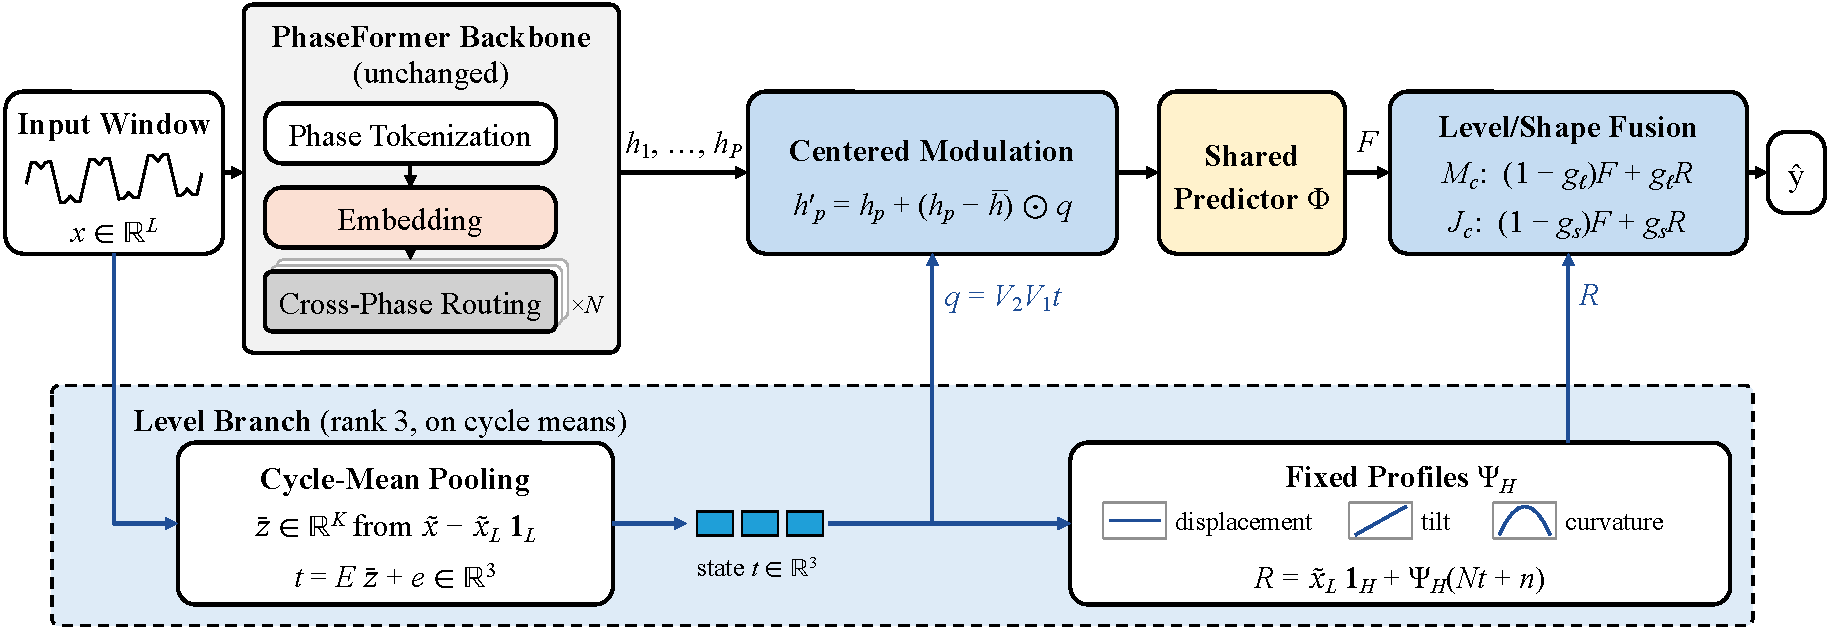
\includegraphics[width=\textwidth]{figures/la_overview.pdf}
\caption{\sysLA. The \sysname backbone and the shared predictor are unchanged and keep their colors of Fig.~\ref{fig:overview}; the new components are blue. A rank-3 level branch reads the anchored cycle means and writes onto three fixed horizon profiles; its state $t$ drives a centered modulation of the final phase latents; the two forecasts are fused with separate level and shape gates.}
\label{fig:la_overview}
\end{figure*}

\subsection{Level branch on cycle means}
\label{sec:ext_branch}

Let $\tilde x_L$ be the last value of the normalized window. The branch pools the anchored window $\tilde x-\tilde x_L\one_L$ to its $K$ cycle means $\bar z\in\mathbb R^K$ and maps them to a rank-3 state,
\begin{equation}
t=E\bar z+e\in\mathbb R^3,\qquad
R=\tilde x_L\one_H+\Psi_H\,(Nt+n),
\label{eq:branch}
\end{equation}
where $\Psi_H\in\mathbb R^{H\times3}$ holds the displacement, tilt and curvature profiles, the discrete orthogonal polynomials of degree $0,1,2$ on the forecast grid, normalized to unit root mean square, so that its first column is $\one_H$ and the other two are horizon-centered. $\Psi_H$ is fixed; only $E\in\mathbb R^{3\times K}$, $e$, $N\in\mathbb R^{3\times3}$ and $n$ are learned. The design follows Theorem~\ref{thm:complement} term by term: the input contains the Bayes level functional, which is a function of the cycle means; the output spans the displacement profile and two smooth profiles; the rank is the number of profiles; and the anchor gives the branch an exactly shift-equivariant level channel that, unlike the phase path's, is not bounded by an envelope. $N$ and $n$ are initialized to zero, so the branch initially forecasts the last value. The branch has $3K+3+9+3=105$ parameters at $K=30$, \emph{independently of the horizon}.

\subsection{Level and shape fusion}
\label{sec:ext_fusion}

Let $F$ be the phase forecast and $R$ the branch forecast, both in normalized units. For every future cycle, the level of the fused forecast and its within-cycle shape are mixed with separate gates,
\begin{equation}
\begin{gathered}
M_c\hat{\tilde y}=(1-g_\ell)M_cF+g_\ell M_cR,\\
J_c\hat{\tilde y}=(1-g_s)J_cF+g_sJ_cR,
\end{gathered}
\label{eq:fusion}
\end{equation}
with $g_\ell=\operatorname{sigmoid}(\omega)$ and $g_s=\operatorname{sigmoid}(\omega+\delta)$. Both gates start at $0.2$ ($\delta=0$). Separate gates let the level be handed to the branch, as Theorem~\ref{thm:complement}(c) prescribes, without forcing the branch's smooth profiles into the phase shape. The gates are static: they depend on neither the input nor the time step. They are learned either per channel ($2C$ parameters) or shared across channels (two parameters); Section~\ref{sec:ext_setup} gives the rule that selects between the two for each dataset.

\subsection{Centered amplitude modulation}
\label{sec:ext_modulation}

Let $h_1,\dots,h_P\in\mathbb R^d$ be the phase latents after the last routing layer. Before the shared predictor, \sysLA modulates them as in \equref{eq:modulation} with a vector driven by the branch state,
\begin{equation}
h'_p=h_p+(h_p-\bar h)\odot q,\qquad q=V_2V_1\,t,
\label{eq:la_modulation}
\end{equation}
with $V_1\in\mathbb R^{k\times3}$, $V_2\in\mathbb R^{d\times k}$, $k=\min(w,3,d)$, no biases, and $V_2$ initialized to zero; the width $w$ is $2$ by default, and the grid search of Section~\ref{sec:ext_setup} also tries $w=4$, which the branch rank caps at $k=3$. The modulation is the complement of Theorem~\ref{thm:amplitude}: centering over the phases is what makes it invisible to every future cycle mean (part~c), and the level-driven factor $q$ scales the shape budget of the phase path (part~d). The branch state $t$ is the natural driver because Theorem~\ref{thm:complement} makes it a linear read of the level forecast. A modulation of width $k=1$ already contains the construction of Theorem~\ref{thm:amplitude}(d); $k=2$ also allows the tilt state to modulate the shape. The modulation has $k(3+d)$ parameters.

\subsection{Properties and cost}
\label{sec:ext_properties}

\fakeparagraph{Exact nesting}
With $V_2=0$ the modulation is the identity, so \sysLA reduces exactly to \sysL; with $g_\ell=g_s=0$ it reduces exactly to \sysname. Because $V_2$ is initialized to zero, \sysLA and \sysL have identical forecasts at initialization when they are built from the same random state, which our experiments use to pair them.

\fakeparagraph{Preserved guarantees}
Theorem~\ref{thm:amplitude}(c) applies to \equref{eq:la_modulation} for every value of $V_1$, $V_2$ and $t$, so the level path of \sysLA is exactly that of \sysL. Theorems~\ref{thm:level_envelope}(b,c) and~\ref{thm:complement} hold for its phase path. The fusion~\equref{eq:fusion} needs whole forecast cycles, which all benchmark horizons provide.

\fakeparagraph{Parameters and complexity}
The branch adds 105 parameters and the modulation $k(3+d)$, so together they add between 119 and 367 parameters across all 28 settings, independently of the horizon; the gates add two parameters per channel, or two in total when shared. The branch costs $O(L)$ per channel for pooling and $O(K+H)$ for the readout, and the modulation $O(Pd)$, against the $O\big(N((P+M)d^2+MPd)+d(L+H)\big)$ of \sysname, so the overall complexity remains linear in the input and output lengths and in the number of sensors.
}

\section{Experiments}
\label{sec:exp}

\blue{Section~\ref{sec:exp_main} gives the setup. Sections~\ref{sec:exp_results} and~\ref{sec:exp_efficiency} compare \sysname and \sysLA with the baselines in accuracy and cost, and Section~\ref{sec:exp_ablation} analyzes the components of \sysname. Section~\ref{sec:exp_theory} then tests the theory of Section~\ref{sec:theory} on trained checkpoints, and Section~\ref{sec:exp_ladder} attributes the gains of \sysLA to its two components.}

\subsection{\blue{Setup}}
\label{sec:exp_main}

\blue{The code is available at} \url{\codeurl}.

\fakeparagraph{Datasets and Setup}
Experiments are performed on seven widely used long-term time series forecasting datasets: 
\textit{ETTh1}, 
\textit{ETTh2}, 
\textit{ETTm1}, 
\textit{ETTm2}\footnote{\url{https://github.com/zhouhaoyi/ETDataset}}, 
\textit{Weather}\footnote{\url{https://www.bgc-jena.mpg.de/wetter/}}, 
\textit{Electricity}\footnote{\url{https://archive.ics.uci.edu/ml/datasets}}, 
and \textit{Traffic}\footnote{\url{https://pems.dot.ca.gov/}}, 
covering a diverse range of real-world scenarios.
The details of the datasets are provided in \blue{the electronic supplement}.
Following prior works~\citep{nie2023patchtst, zhang2023crossformer, huang2025timebase}, we adopt a 6:2:2 split for the ETT datasets and a 7:1:2 split for the other datasets. 
For \sysname, we report the average results over three random seeds, while for the other baselines we follow their official implementations and released code. 
We evaluate the forecasting \textbf{accuracy} of all tested models using mean squared error (MSE) and mean absolute error (MAE), 
and assess \textbf{efficiency} in terms of floating-point operations (FLOPs) and the number of parameters (Params).

\fakeparagraph{Baselines and Implementation Details}
% We evaluate our approach against eight competitive baselines, encompassing both state-of-the-art Transformer architectures and parameter-efficient forecasting models.  
\revised{
We evaluate our approach against eight competitive baselines, following the standard non-pretraining setting where all models are trained and evaluated directly on domain-specific datasets. 
The baselines span both state-of-the-art Transformer-based architectures and recent parameter-efficient forecasting models.
}
We compare our method with PatchTST \citeyearpar{nie2023patchtst}, iTransformer \citeyearpar{liu2023itransformer}, Crossformer \citeyearpar{zhang2023crossformer}, FEDformer \citeyearpar{zhou2022fedformer}, TimeBase \citeyearpar{huang2025timebase}, SparseTSF \citeyearpar{lin2024sparsetsf}, FITS \citeyearpar{fits2024}, and TimeMixer \citeyearpar{timemixer24}.
Among these, PatchTST, Crossformer, and TimeMixer are patch-based; SparseTSF is phase-based; TimeBase integrates patch and phase paradigms; FITS and FEDformer are frequency-domain; and iTransformer models the full sequence directly.
For all baselines, we adopt the recommended configurations provided in their official implementations\revised{, keeping hyperparameters aligned with ~\cite{huang2025timebase}.}
The model is optimized using the Adam optimizer with a fixed learning rate of $1 \times 10^{-3}$.  
Following the settings from efficiency-oriented works~\citep{huang2025timebase, lin2024sparsetsf, fits2024}, the look-back length is set to 720 time steps.
More implementation details are provided in \blue{the electronic supplement}.

\blue{
\fakeparagraph{Setup for \sysLA}
\label{sec:ext_setup}
\sysLA uses the \sysname backbone of each setting (a setting is one dataset with one horizon, 28 in total) with the components of Section~\ref{sec:extension}. It is trained from scratch with the Huber loss, at most 30 epochs with early stopping on the validation loss (patience 8), with three seeds (2021--2023). The Huber loss is chosen for its linear tail, which keeps sharp level shifts from dominating the gradient and stabilizes training. All runs of \sysL and \sysLA use the input length $L=720$, the period $P=24$, and the seven datasets and four horizons above. \sysL and \sysLA are built from the same random state for each setting and seed, so that they produce identical forecasts at initialization whenever they share the gate initialization (Section~\ref{sec:ext_init}). On the settings that keep the default extension hyperparameters, their differences are therefore due to the modulation alone; on the eight settings where the per-setting search below changed these hyperparameters for \sysLA only, the differences also reflect those changes.

Before the 28-setting runs, we fixed the remaining design choices on the validation split of one setting per dataset (ETTh1-96, ETTh2-720, ETTm1-336, ETTm2-96, Weather-192, Electricity-96 and Traffic-96). The branch decoder was chosen among three variants of the same rank: learned decoders on 30 or 90 pooled values, and the fixed displacement, tilt and curvature profiles of \equref{eq:branch}. The gates were chosen per dataset between per-channel and shared. The rule preferred the variant with the fewest parameters whenever the validation errors were within 0.5\%, and it selected shared gates when they were within 0.1\% of per-channel gates. It selected the fixed profiles for every dataset, and shared gates for ETTh2, ETTm1 and ETTm2. The remaining hyperparameters of the extension --- the modulation width $w$, the learning-rate multiplier of the extension parameters, and the gate initialization --- were selected per setting by a small grid search on the five datasets other than ETTh1 and ETTh2, whose settings keep the default values.

We report \sysLA in two configurations. The \emph{main-table configuration} of Table~\ref{tab:main_results} is the per-setting-tuned deployment configuration: it extends the per-setting search to further extension hyperparameters, including the basis of the level branch and whether the modulation is active at inference, which the search switches off on five settings (Appendix~\ref{app:la_config}). The \emph{protocol configuration} keeps one branch design, the fixed profiles, on every setting and the modulation always active at inference, so that the mechanism analyses of Sections~\ref{sec:exp_theory} and~\ref{sec:exp_ladder} are defined in the same way on all 28 settings; it is the instrument of these controlled attributions rather than a deployment recipe. Those sections compare it with \sysL and with the \sysname backbone retrained under the same protocol, which we call \sysname (retrained), as opposed to \sysname (conference), the result of the conference version. The dataset averages of the two \sysLA configurations differ by between 0.3\% and 2\%.
}

\subsection{\blue{Main Results}}
\label{sec:exp_results}

We conduct a joint evaluation of model efficiency and predictive accuracy. 
The comparative analysis highlights that the proposed \textit{\sysname} establishes an improved effectiveness-efficiency tradeoff in terms of parameter scale and error metrics.

\begin{table*}[t]
\centering
\caption{
Main results for long-term forecasting.
\blue{The input length is $L=720$, and results are averaged over the horizons $H\in\{96,192,336,720\}$.}
The best results are shown in \best{bold}, and the second-best in \second{underline}.
\blue{The \sysname row is \sysname (conference). \sysLA uses the main-table configuration (Section~\ref{sec:ext_setup}) and is averaged over three seeds; bold and underline marks are assigned among the baselines and \sysname only, so the \sysLA row is reported as a reference and carries no marks by design, even where it is the best entry.}
}
\label{tab:main_results}
\footnotesize
\setlength{\tabcolsep}{3.6pt}
\begin{tabular}{l|cc|cc|cc|cc|cc|cc|cc}
\hline
\multirow{2}{*}{Model}
& \multicolumn{2}{c|}{ETTh1}
& \multicolumn{2}{c|}{ETTh2}
& \multicolumn{2}{c|}{ETTm1}
& \multicolumn{2}{c|}{ETTm2}
& \multicolumn{2}{c|}{Electricity}
& \multicolumn{2}{c|}{Traffic}
& \multicolumn{2}{c}{Weather} \\
\cline{2-15}
 & MSE & MAE & MSE & MAE & MSE & MAE & MSE & MAE & MSE & MAE & MSE & MAE & MSE & MAE \\
\hline
\blue{\sysLA} & \blue{0.401} & \blue{0.418} & \blue{0.341} & \blue{0.387} & \blue{0.351} & \blue{0.379} & \blue{0.248} & \blue{0.313} & \blue{0.159} & \blue{0.250} & \blue{0.392} & \blue{0.252} & \blue{0.219} & \blue{0.256} \\
\hline
\sysname & \best{0.403} & \best{0.415} & 0.346 & 0.388 & \best{0.346} & \best{0.374} & \best{0.250} & \best{0.313} & \best{0.160} & \best{0.250} & \best{0.386} & \best{0.249} & \best{0.223} & \best{0.260} \\
PatchTST & 0.420 & 0.439 & \second{0.344} & 0.390 & \second{0.354} & 0.383 & 0.251 & 0.319 & 0.169 & 0.265 & \second{0.394} & \second{0.266} & \second{0.223} & 0.264 \\
iTransformer & 0.453 & 0.467 & 0.392 & 0.422 & 0.370 & 0.401 & 0.278 & 0.337 & \second{0.165} & 0.263 & 0.406 & 0.290 & 0.233 & 0.273 \\
Crossformer & 0.517 & 0.512 & 1.468 & 0.867 & 0.390 & 0.417 & 0.392 & 0.426 & 0.180 & 0.273 & 0.545 & 0.282 & 0.255 & 0.304 \\
FEDformer & 0.523 & 0.523 & 0.428 & 0.469 & 0.438 & 0.465 & 0.401 & 0.452 & 0.235 & 0.348 & 0.638 & 0.400 & 0.354 & 0.393 \\
TimeBase & \second{0.404} & \second{0.416} & 0.347 & 0.397 & 0.356 & \second{0.380} & \best{0.250} & \second{0.314} & 0.167 & \second{0.258} & 0.418 & 0.278 & 0.227 & \second{0.262} \\
SparseTSF & 0.406 & 0.418 & 0.345 & \second{0.383} & 0.362 & 0.383 & 0.252 & 0.316 & 0.168 & 0.263 & 0.413 & 0.280 & 0.243 & 0.285 \\
FITS & 0.419 & 0.435 & \best{0.334} & \best{0.382} & 0.359 & 0.382 & 0.285 & 0.336 & 0.172 & 0.270 & 0.410 & 0.290 & 0.241 & 0.283 \\
TimeMixer & 0.452 & 0.474 & 0.386 & 0.425 & 0.383 & 0.413 & 0.314 & 0.367 & 0.171 & 0.273 & 0.421 & 0.298 & 0.237 & 0.281 \\
\hline
\end{tabular}
\end{table*}

\begin{figure*}[t]
    \centering
    % 子图1 - Traffic FLOPs
    \begin{subfigure}{0.24\textwidth}
        \centering
        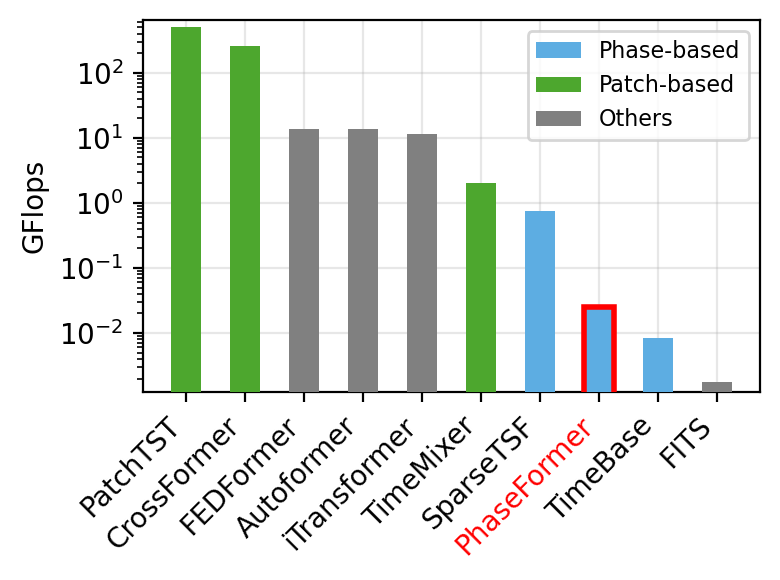
\includegraphics[width=\linewidth]{figures/flops_traffic.png}
        \caption{FLOPs on Traffic}
        \label{fig:traffic_flops}
    \end{subfigure}
    % 子图2 - Traffic Params
    \begin{subfigure}{0.24\textwidth}
        \centering
        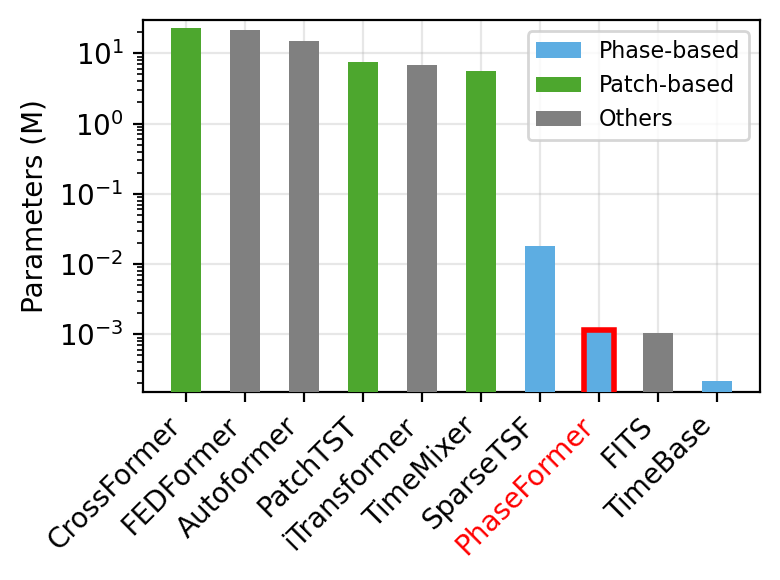
\includegraphics[width=\linewidth]{figures/params_traffic.png}
        \caption{Params on Traffic}
        \label{fig:traffic_params}
    \end{subfigure}
    % 子图3 - Electricity FLOPs
    \begin{subfigure}{0.24\textwidth}
        \centering
        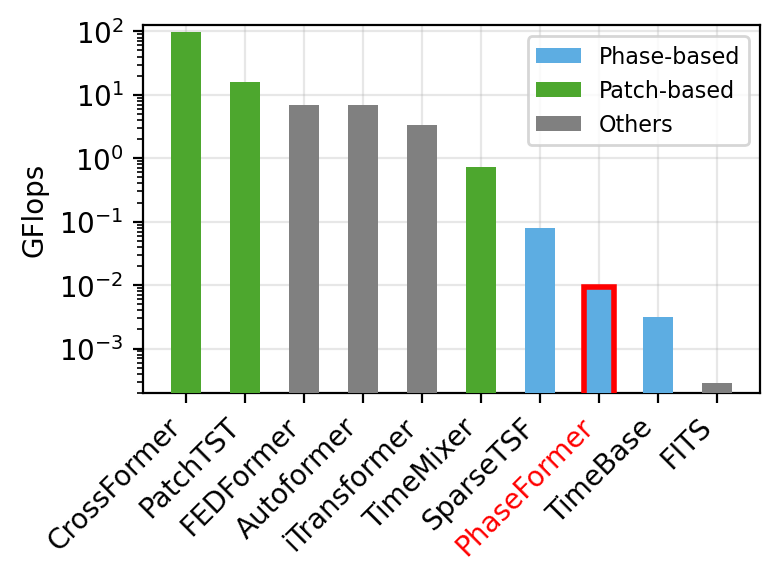
\includegraphics[width=\linewidth]{figures/flops_electricity.png}
        \caption{FLOPs on Electricity}
        \label{fig:electricity_flops}
    \end{subfigure}
    % 子图4 - Electricity Params
    \begin{subfigure}{0.24\textwidth}
        \centering
        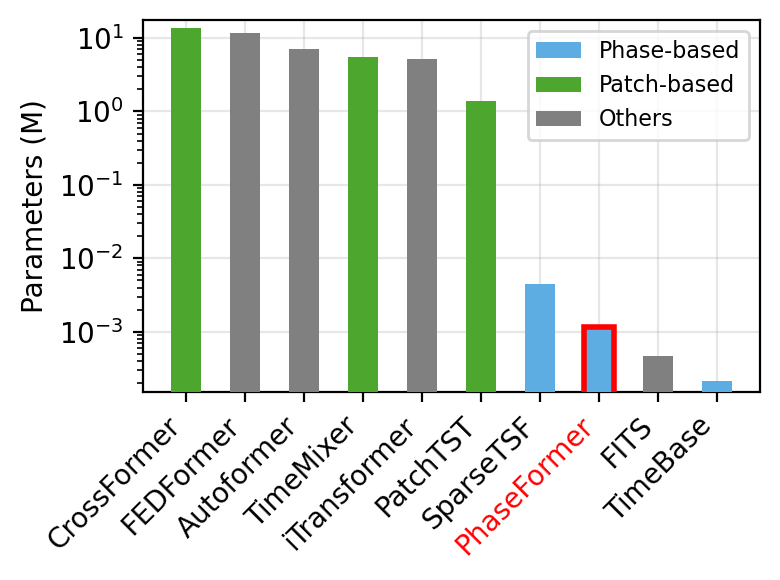
\includegraphics[width=\linewidth]{figures/params_electricity.png}
        \caption{Params on Electricity}
        \label{fig:electricity_params}
    \end{subfigure}
    \caption{
    Comparison of FLOPs and parameter counts across models on the Traffic and Electricity\revised{, using an input length of 720 steps and predicting 96 future steps}.
    Patch-based models are shown in green, phase-based models in blue, and other models in gray.
    }
    \label{fig:flops_params_visualization}
\end{figure*}


We evaluate the predictive accuracy of \sysname and the baseline methods on seven datasets. 
\tabref{tab:main_results} reports the average prediction errors across four forecasting horizons, with detailed results provided in \blue{the electronic supplement}.
\blue{Overall, \sysname attains the best average MSE on six of the seven datasets, with the clearest margins on the two large sensor networks: on Electricity it reduces the MSE by 3.0\% relative to the runner-up, iTransformer, and on the largest dataset, Traffic, by 2.0\% relative to PatchTST and by 7.7\% relative to TimeBase, underscoring its robustness on large-scale and heterogeneous data.}
\blue{The only exception is ETTh2, where FITS leads (0.334) and \sysname is within 0.002 of the second-best MSE (PatchTST, 0.344) and third in MAE.}
A closer examination reveals that patch-based baselines, including PatchTST, Crossformer, and TimeMixer, exhibit performance degradation on \blue{Electricity}.
\blue{The electronic supplement adds CycleNet to the comparison: on Electricity it attains a lower dataset average than both \sysname and \sysLA (0.157 against 0.160 and 0.159 in the full per-horizon tables of the supplement). We position this as a point on the efficiency trade-off rather than a like-for-like gap: CycleNet carries 472K parameters on Electricity and 563K on Traffic against the 1.16K of \sysname on both --- several hundred times more, a cost that grows with the number of channels through its learnable per-channel recurrent cycles (see the per-model parameter and FLOPs comparison in the electronic supplement).}

\blue{
\fakeparagraph{Results of \sysLA}
Table~\ref{tab:main_results} adds \sysLA, averaged over three seeds; per-horizon results with standard deviations are in Table~\ref{tab:la_full}. Against \sysname (conference), \sysLA improves the MSE on five of the seven dataset averages, by up to 1.6\% (Weather), and on 17 of the 28 settings; the MAE improves on 12 settings and four dataset averages (all comparisons on unrounded averages). These gains are conservative: the shared training protocol of the extension places \sysname (retrained) above its conference error on every dataset. Against \sysname (retrained), \sysLA improves the MSE on ETTh2, ETTm2 and Weather at every horizon by more than one seed standard deviation (Table~\ref{tab:la_full}), and on ETTm1 and Traffic the two models match: \sysname (retrained) averages 0.352 and 0.392 there, the \sysLA row 0.351 and 0.392. Section~\ref{sec:exp_theory} shows that ETTh2, ETTm2 and Weather are where the level envelope binds, and Section~\ref{sec:exp_ladder} attributes the gains to the two components under one protocol.
}

\subsection{\blue{Efficiency}}
\label{sec:exp_efficiency}

We evaluate the computational overhead of all models, with detailed results in \blue{the electronic supplement}.
\figref{fig:flops_params_visualization} shows the FLOPs and the number of parameters of all tested models on the Electricity and Traffic.
Overall, phase-based models incur lower overhead than patch-based ones.
On the Traffic dataset, \sysname achieves a FLOPs reduction of about 99.99\% over PatchTST and Crossformer.
Beyond patch-based baselines, it also outperforms other phase-based models like SparseTSF, consistently delivering high efficiency.
This stems from the \blue{stability} of phase tokens over time (\secref{sec:mot_stability}), making them inherently more efficient to process. 
Taken together with the previous accuracy evaluations, these results \blue{show} that \sysname provides an efficient yet effective solution, delivering superior performance on complex datasets.
\blue{The extension keeps this efficiency profile. Over \sysname, the level branch and the modulation of \sysLA add between 119 and 679 parameters in all 28 settings of the main-table configuration. The fusion gates add two parameters in total when they are shared and two per channel otherwise (1{,}724 on Traffic); they are the only component of the extension whose size grows with the number of sensors. Including them, the extension adds at most about 2.1K parameters, the largest increment being on Traffic (Section~\ref{sec:complexity} and Appendix~\ref{app:la_config}). Its added computation is linear in the input length and is dominated by the cost of the backbone.}
\blue{Measured on a single A800 GPU (fp32, batch 32, $L{=}720$), the extension adds between $0.09\%$ and $0.23\%$ to the FLOPs of the \sysname backbone on Traffic and Electricity, and between $3.9\%$ and $10.5\%$ to its latency: the added operations --- gates, fusions and pooling --- are element-wise and therefore memory-bound rather than compute-bound. The ratio falls as the backbone grows; on the smallest backbone (ETTh2-720, 718 parameters) the same absolute overhead amounts to about $37\%$ of its FLOPs and $71\%$ of its latency, the forward pass remaining below $2$\,ms.}

\subsection{\blue{Analysis of \sysname}}
\label{sec:exp_ablation}

\subsubsection{\blue{Ablation Studies}}

\fakeparagraph{Varying the Number of Routers}
We systematically evaluate the impact of different number of routers $M$ on model performance, with results summarized in \figref{fig:router_number_visualization}.
The experiments indicate that across three datasets, the model’s prediction error generally decreases as the number of routers $M$ increases, before eventually stabilizing or slightly rising.
It is worth noting that the best performance is usually achieved when $M \in \{4,8\}$, which is much smaller compared to the actual number of phase tokens, $L_{\text{phase}} = 24$.
This observation indicates that the phase token spans an inherently low-dimensional space, so only a small number of routers is sufficient to effectively capture and represent its underlying structure\blue{, in line with Insight~2 (Section~\ref{sec:mot_stability}), by which two dimensions explain over 90\% of the variance of phase tokens}.
More detailed results are provided in \blue{the electronic supplement}.

\begin{figure*}[t]
    \centering
    % 子图1
    \begin{subfigure}{0.32\textwidth}
        \centering
        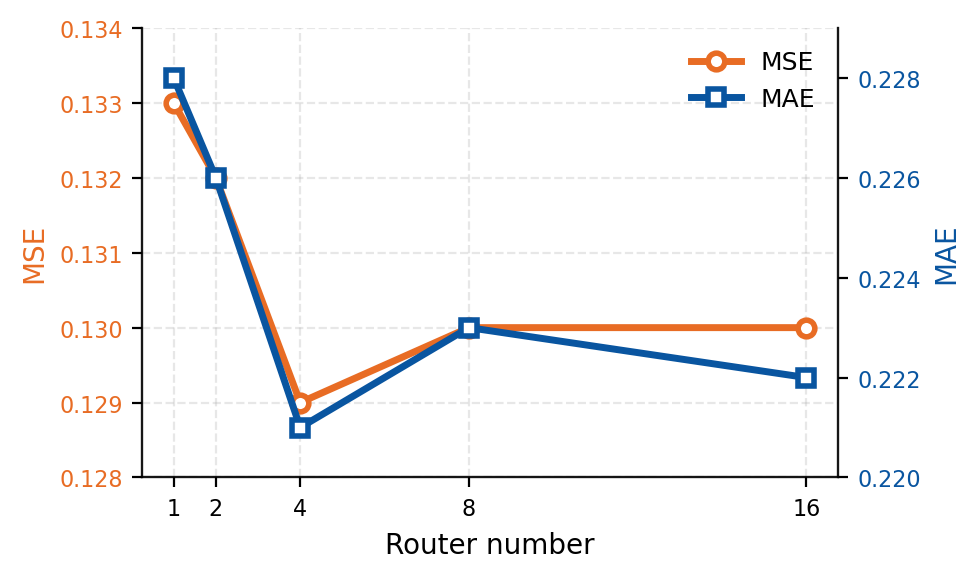
\includegraphics[width=\linewidth]{figures/router_number_effect_electricity_lines.png}
        \caption{Electricity}
        \label{fig:electricity}
    \end{subfigure}
    % 子图2
    \begin{subfigure}{0.32\textwidth}
        \centering
        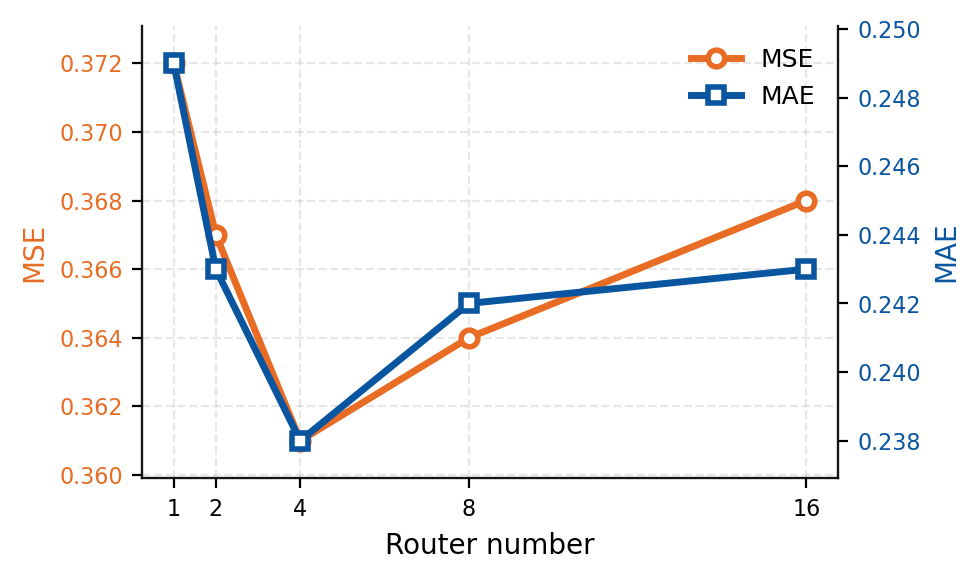
\includegraphics[width=\linewidth]{figures/router_number_effect_traffic_lines.png}
        \caption{Traffic}
        \label{fig:traffic}
    \end{subfigure}
    % 子图3
    \begin{subfigure}{0.32\textwidth}
        \centering
        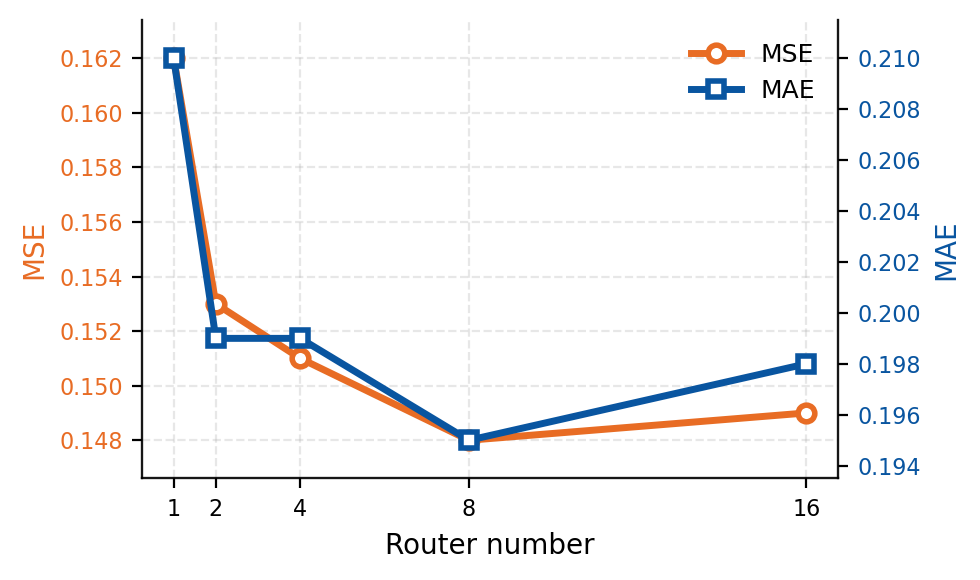
\includegraphics[width=\linewidth]{figures/router_number_effect_weather_lines.png}
        \caption{Weather}
        \label{fig:Weather}
    \end{subfigure}
    
    \caption{Effect of varying the number of routers $M$ on forecasting performance on three datasets.}
    \label{fig:router_number_visualization}
\end{figure*}



\begin{table*}[t]
\centering
\caption{Cross-Phase Routing layer ablation. Each cell reports MSE, MAE, and FLOPs. Lower is better for all metrics. FLOPs are reported in millions (MFLOPs). The best results are highlighted with \best{Bold}, and the second-best results with \second{Underlined}.}
\label{tab:ablation_phase}
\footnotesize
\begin{tabular}{c|ccc|ccc|ccc|ccc}
\hline
\multirow{2}{*}{Dataset}
& \multicolumn{3}{c|}{\textbf{\sysname}} 
& \multicolumn{3}{c|}{\textbf{w/ FullAttention}} 
& \multicolumn{3}{c|}{\textbf{w/ LinearMixing}} 
& \multicolumn{3}{c}{\textbf{w/o Routing}} \\
\cline{2-13}
& MSE & MAE & FLOPs 
& MSE & MAE & FLOPs 
& MSE & MAE & FLOPs 
& MSE & MAE & FLOPs \\
\hline
Weather 
& \best{0.1503} & \best{0.1971} & 3.119 
& \second{0.1527} & \second{0.2005} & 3.202 
& 0.1700 & 0.2226 & \second{0.920} 
& 0.1907 & 0.2406 & \best{0.783} \\
\hline
Electricity 
& \best{0.1290} & \best{0.2209} & 42.213 
& \second{0.1295} & \second{0.2217} & 48.951 
& 0.1403 & 0.2334 & \second{14.068} 
& 0.1423 & 0.2365 & \best{11.972 } \\
\hline
Traffic     
& \best{0.3721} & \best{0.2475} & 113.356 
& \second{0.3791} & \second{0.2513} & 131.452 
& 0.3842 & 0.2532 & \second{37.776}
& 0.3892 & 0.2584 & \best{32.149}  \\
\hline
\end{tabular}
\end{table*}




\fakeparagraph{Effectiveness of Cross-Phase Routing} 
To assess the contribution of the cross-phase routing layer, we compare four variants of the model: 
\textbf{\sysname}, which adopts the original cross-phase routing layer; 
\textbf{w/ FullAttention}, which substitutes the cross-phase routing layer with a full attention mechanism;
\textbf{w/ LinearMixing}, which replaces the cross-phase routing layer with a linear layer; and 
\textbf{w/o Routing}, which directly projects each phase into its own future.
All other experimental settings are kept identical across these variants. 

As summarized in \tabref{tab:ablation_phase}, \sysname consistently outperforms \textbf{w/ LinearMixing} and \textbf{w/o Routing}, indicating that explicit cross-phase routing is crucial for modeling periodic dynamics. Moreover, \sysname not only incurs less \blue{computation}, but also achieves lower prediction error than \textbf{w/ FullAttention}, showing that the routing layer is both efficient and effective. We attribute these gains to operating in a low-dimensional phase token space, which concentrates informative interactions and reduces cost.

\revised{
\subsubsection{Sensitivity Analysis of Phase Length Choices}
\label{sec:phase_length}

\begin{table}[t]
\centering
\begin{tabular}{ccc}
\hline
\textbf{Phase Length} & \textbf{MSE} & \textbf{MAE} \\
\hline
24 & 0.3619 & 0.2384 \\
12 & 0.3960 & 0.2765 \\
8  & 0.4032 & 0.2801 \\
28 & 0.4063 & 0.2753 \\
21 & 0.4184 & 0.2970 \\
\hline
\end{tabular}
\caption{Comparison of forecasting performance under different phase lengths on the Traffic dataset (\blue{$L=720$, $H=96$}).}
\label{tab:phase_length}
\end{table}
\sysname automatically determines the phase length through frequency-domain analysis (see \blue{the electronic supplement}), extracting salient periodic components directly from the data.
To assess its sensitivity to phase length, we conduct experiments on the Traffic dataset. Its frequency spectrum contains several clear periodic components (see \figref{fig:spectrum_traffic}). Based on spectral amplitudes, we select the top five candidate phase lengths and run \sysname for forecasting. The results are shown in \tabref{tab:phase_length}.

\begin{figure}[t]
    \centering
    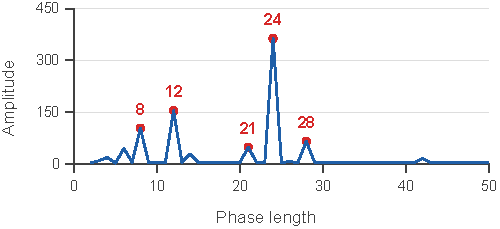
\includegraphics[width=\linewidth]{figures/spectrum_traffic.pdf}
    \caption{The spectrum calculated on the Traffic dataset. The top-5 phase length is 24, 12, 8, 28, 21.}
    \label{fig:spectrum_traffic}
\end{figure}

The experiments show that the model performs best when the phase length is 24, corresponding to the dominant spectral component. \blue{The errors of the five candidates increase exactly in the order of their spectral amplitudes (\figref{fig:spectrum_traffic}), so the strongest spectral component is also the most accurate phase length.}
These findings demonstrate that \sysname effectively captures the dataset’s primary periodic structure.
}

\subsubsection{Case Study}
\label{sec:exp_case}
We select one sample from Traffic dataset, comprising an input sequence of length 720 and an output sequence of length 96 (816 time steps in total). 
The input sequence is fed into \sysname, and we record the attention-weight matrices at the first cross-phase routing layer during both aggregation (Phase$\rightarrow$Router) and distribution (Router$\rightarrow$Phase).
As shown in \figref{fig:sender} and \figref{fig:receiver}, both attention patterns exhibit clear local similarity: adjacent phases tend to be assigned to the same routers and to receive attention from similar routers.
This indicates that the routing mechanism captures temporally consistent phase relationships. 
Meanwhile, the attention weights reveal that certain phases share similar attentive patterns.
To analyze this further, we focus on three phases with distinct attentive patterns and \blue{visualize} them in \figref{fig:traffic_data_visualization}.
These phases display different temporal behaviors: Phase 5 remains relatively stable over long horizons, whereas Phase 9 and Phase 1 both exhibit a pronounced 7-day periodicity but with opposite trends.
The differing patterns of these phase tokens suggest that the router structure not only distinguishes among phase tokens but also effectively models their periodicity and trend characteristics.


\begin{figure*}[t] 
  \centering
  \begin{subfigure}{0.24\linewidth}
    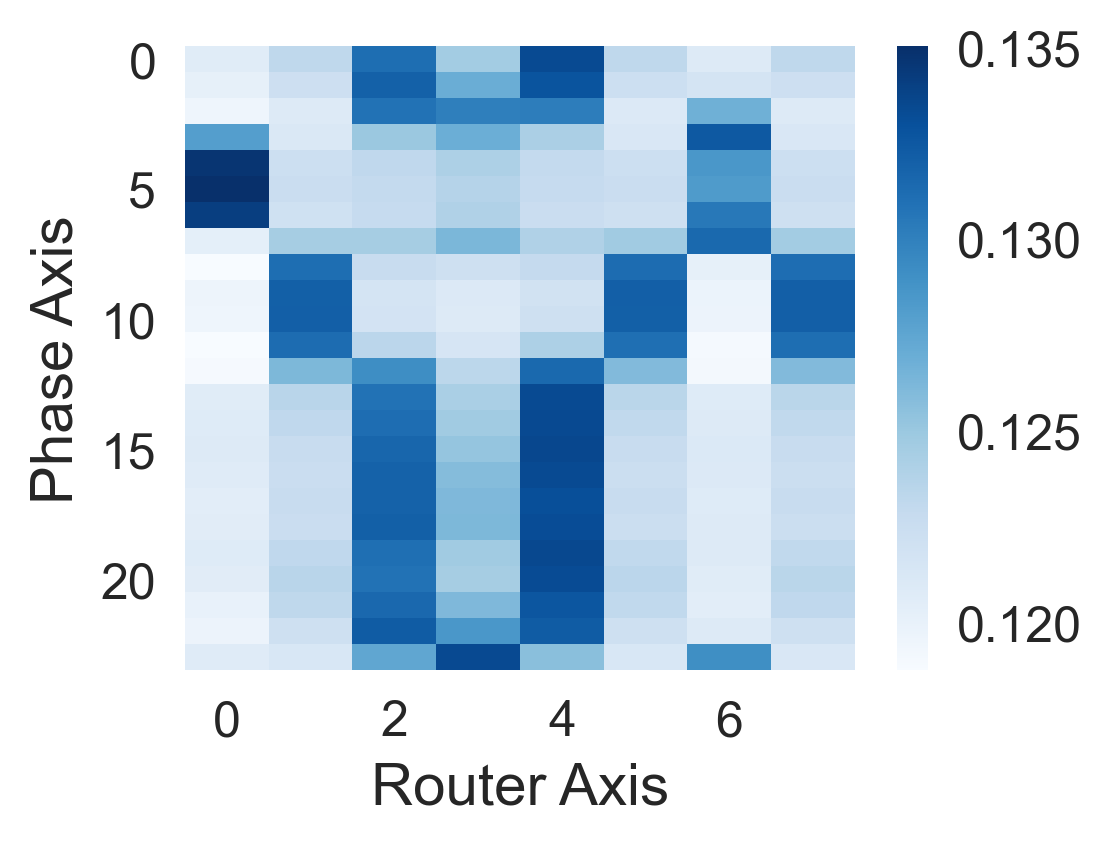
\includegraphics[width=\linewidth]{figures/attention_layer_0_sender_var4.png}
    \caption{Aggregation Weights}
    \label{fig:sender}
  \end{subfigure}%
  \hfill
  \begin{subfigure}{0.24\linewidth}
    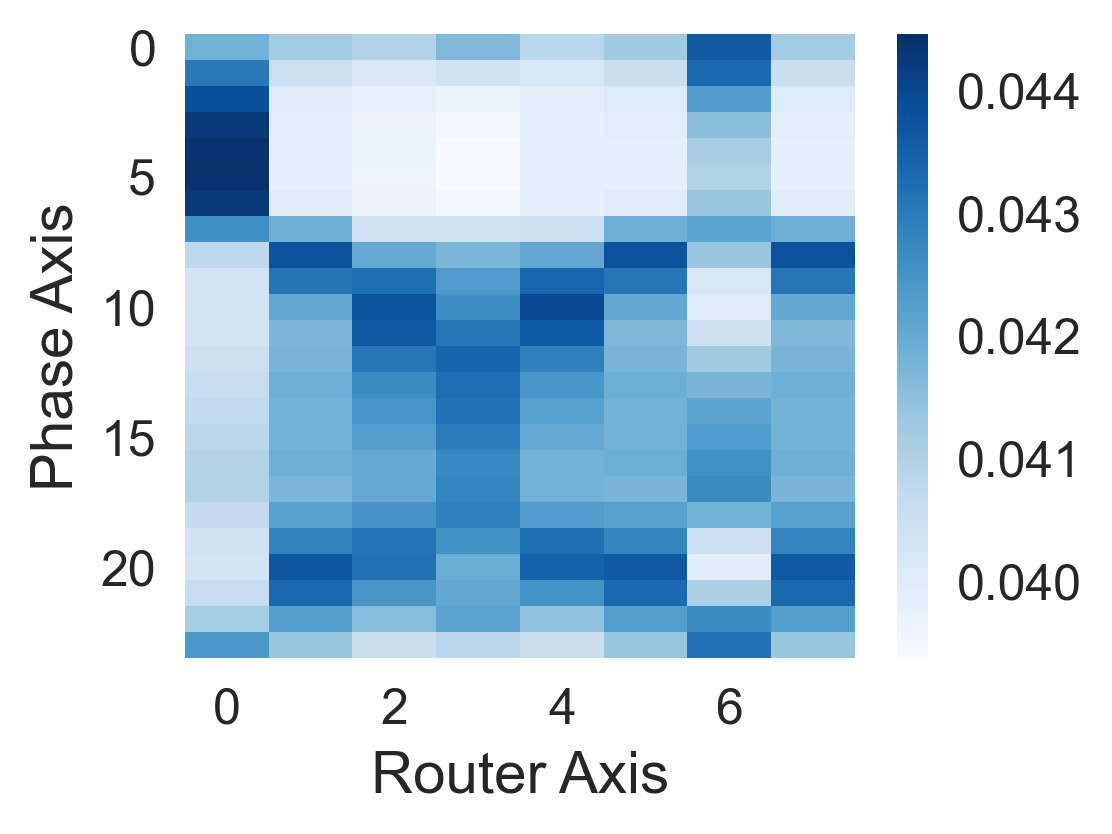
\includegraphics[width=\linewidth]{figures/attention_layer_0_receiver_var4.png}
    \caption{Distribution Weights}
    \label{fig:receiver}
  \end{subfigure}
  \hfill
  \begin{subfigure}{0.48\linewidth}
    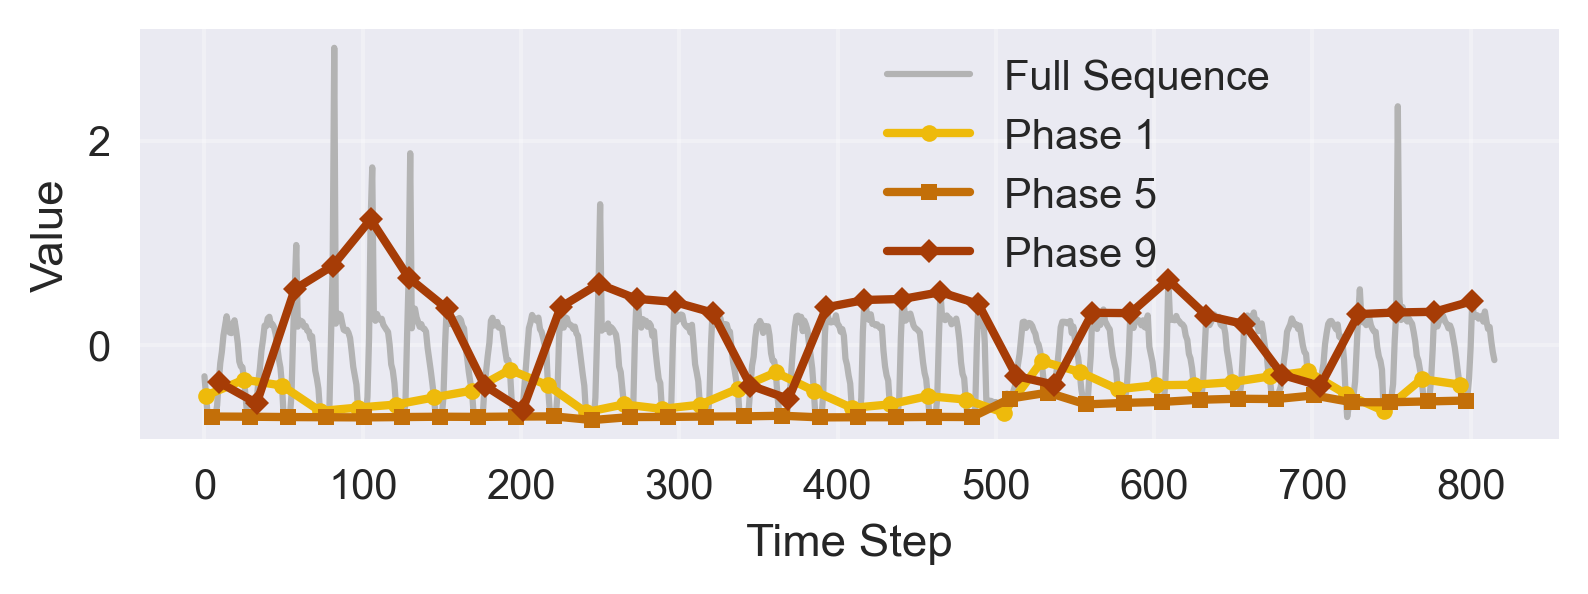
\includegraphics[width=\linewidth]{figures/sequence_with_phase_curves_sample_0_feature_0.png}
    \caption{Visualization of three selected phase tokens}
    \label{fig:traffic_data_visualization}
  \end{subfigure}%
  \caption{Case study on a sample from the Traffic dataset. 
  (a) Attention weight matrix during Phase-to-Router aggregation. 
  (b) Attention weight matrix during Router-to-Phase distribution. 
  Both matrices capture the association between 8 routers and 24 input phases. 
  (c) Visualization of three representative phases (1, 5, and 9), each represents a distinct attentive pattern with routers.} 
  \label{fig:case_study_wrap_all}
\end{figure*}


\blue{
\subsection{Validating the Theory}
\label{sec:exp_theory}

Section~\ref{sec:theory} argues in four steps. Step~(i), that \sysname can represent level drift, is established by construction (Proposition~\ref{prop:capability}). Steps~(ii)--(iv) make predictions that can be checked on trained checkpoints: that the envelopes hold on every checkpoint and bind where the demands of the data exceed them, and that the branch takes over the level there (Section~\ref{sec:exp_envelopes}); that the modulation preserves the cycle means and reads the level (Section~\ref{sec:exp_mechanism}); and that a few fixed profiles suffice for the level branch (Section~\ref{sec:exp_capacity}). Section~\ref{sec:exp_ladder} then measures what each component gains.

\subsubsection{Envelopes and Level Hand-over on Trained Checkpoints}
\label{sec:exp_envelopes}

The constants of Theorems~\ref{thm:level_envelope} and~\ref{thm:amplitude} are functions of the weights, so they can be read from every trained checkpoint, and the demands are functions of the data. Table~\ref{tab:envelope} reports both for the \sysLA checkpoints (averaged over the four horizons), together with the level demand $\Lambda$ and the amplitude demand $\Omega$ of every test window.

\begin{table}[t]
\blue{
\centering
\caption{Envelopes of the phase path on trained \sysLA checkpoints (protocol configuration; averages over the horizons; modulation switched off). $C_1$, $B_\varphi$: half-width of the level envelope and amplitude envelope, read from the weights; $g_s$: shape gate; outside $\mathcal I_\varphi$: share of test windows whose level demand $\Lambda$ lies outside the level envelope; floor/MSE: error floor~\equref{eq:level_floor} as a share of the test MSE; $\Omega$ over env.: share of windows whose amplitude demand exceeds $(1-g_s)B_\varphi$.}
\label{tab:envelope}
\footnotesize
\setlength{\tabcolsep}{2.6pt}
\begin{tabular}{lcccccc}
\toprule
Dataset & $C_1$ & $B_\varphi$ & $g_s$ & outside $\mathcal I_\varphi$ & floor/MSE & $\Omega$ over env. \\
\midrule
ETTh1 & 1.35 & 1.37 & 0.23 & 2.5\% & 0.08\% & 14.8\% \\
ETTh2 & 1.07 & 1.08 & 0.25 & 19.4\% & 5.0\% & 31.8\% \\
ETTm1 & 1.86 & 1.99 & 0.35 & 3.5\% & 0.27\% & 2.2\% \\
ETTm2 & 1.39 & 1.47 & 0.26 & 12.5\% & 10.6\% & 5.7\% \\
Weather & 1.41 & 1.61 & 0.68 & 20.7\% & 11.6\% & 27.6\% \\
Electricity & 3.80 & 3.81 & 0.27 & 0.1\% & 0.5\% & 0.2\% \\
Traffic & 5.23 & 5.25 & 0.21 & 0.0\% & 0.0\% & 0.0\% \\
\bottomrule
\end{tabular}
}
\end{table}

Three observations. First, the level envelope holds exactly as stated: across all 84 checkpoints (28 settings, three seeds), the measured levels of the phase forecast never leave $\mathcal I_\varphi$, the largest observed value of $|\lev(F)-c_0|/C_1$ being $0.74$, so the floors below are conservative. Second, where the envelope binds, it binds in the way the theory predicts. On ETTh2, Weather and ETTm2, between 12\% and 21\% of test windows have a level demand outside the interval, the floor accounts for 5.0\% to 11.6\% of the test MSE, and on ETTh2 and Weather both the share of out-of-envelope windows and the tightness of the interval grow with the horizon (ETTh2: $C_1$ from 1.27 to 0.85 and the outside share from 15\% to 27\% between $H=96$ and $H=720$; Weather: 1.86 to 0.96 and 10\% to 34\%). On the two sensor networks the trained checkpoints developed wide envelopes that almost no test window escapes. Their half-widths, $C_1$ between 3.8 and 5.2, stay below the 5.39 needed to track the level of the last cycle uniformly (Section~\ref{sec:theory_level}), but the level demands of the test windows are smaller, and the floor is at most 0.5\% of the test MSE. The envelopes thus force almost no loss on the phase path there, and Section~\ref{sec:exp_ladder} shows that, under one protocol, the extension changes the error on these datasets by less than 1\%.

Third, the hand-over follows the envelope. The level gate stays near its initialization value on every dataset ($g_\ell$ between 0.20 and 0.26 on average), but what the branch does with its share depends on whether the envelope binds: the correlation between the branch's level and the window's level demand is between $0.40$ and $0.44$ on the four ETT datasets, whose envelopes are narrow ($C_1\le1.86$), and $0.03$ and $-0.01$ on Electricity and Traffic, whose envelopes are wide. The branch tracks the level where the phase path cannot, as Theorem~\ref{thm:complement}(b) predicts.

\begin{table*}[t]
\blue{
\centering
\caption{Ablation ladder, test MSE/MAE averaged over the four horizons and three seeds (protocol configuration, Section~\ref{sec:ext_setup}). \sysname (retrained) is the backbone retrained under this protocol; \sysLA (mod.\ off) is \sysLA with the modulation disabled on the trained checkpoint.}
\label{tab:ladder}
\footnotesize
\setlength{\tabcolsep}{6pt}
\begin{tabular}{lcccccccc}
\toprule
Dataset & \multicolumn{2}{c}{\begin{tabular}[c]{@{}c@{}}\sysname\\(retrained)\end{tabular}} & \multicolumn{2}{c}{\sysL} & \multicolumn{2}{c}{\sysLA} & \multicolumn{2}{c}{\begin{tabular}[c]{@{}c@{}}\sysLA\\(mod.\ off)\end{tabular}} \\
\cmidrule(lr){2-3}\cmidrule(lr){4-5}\cmidrule(lr){6-7}\cmidrule(lr){8-9}
 & MSE & MAE & MSE & MAE & MSE & MAE & MSE & MAE \\
\midrule
ETTh1 & 0.408 & 0.419 & 0.412 & 0.425 & \textbf{0.405} & \textbf{0.421} & 0.414 & 0.429 \\
ETTh2 & 0.354 & 0.396 & \textbf{0.347} & \textbf{0.393} & 0.348 & \textbf{0.393} & 0.352 & 0.396 \\
ETTm1 & \textbf{0.352} & \textbf{0.377} & 0.354 & 0.380 & 0.353 & 0.380 & 0.355 & 0.381 \\
ETTm2 & 0.258 & 0.319 & \textbf{0.253} & \textbf{0.315} & \textbf{0.253} & \textbf{0.315} & 0.257 & 0.318 \\
Weather & 0.227 & 0.262 & 0.221 & 0.257 & \textbf{0.220} & \textbf{0.257} & 0.220 & 0.257 \\
Electricity & 0.161 & 0.251 & \textbf{0.160} & \textbf{0.251} & \textbf{0.160} & \textbf{0.251} & 0.162 & 0.254 \\
Traffic & \textbf{0.392} & \textbf{0.248} & 0.395 & 0.251 & 0.393 & 0.252 & 0.400 & 0.256 \\
\bottomrule
\end{tabular}
}
\end{table*}

\subsubsection{Mechanism of the Modulation}
\label{sec:exp_mechanism}

\fakeparagraph{Synthetic multiplicative series}
We first test Theorem~\ref{thm:amplitude} where the ground truth is known. We generate seven-channel series from \equref{eq:mult_model} with a random-walk level, a sinusoidal daily profile and coupling $\alpha\in\{0,0.25,0.5\}$, and train \sysL and \sysLA from the same initialization (two seeds, 30 epochs). Without coupling ($\alpha=0$), the modulation has nothing to carry and the two models are indistinguishable: \sysLA changes the validation MSE by $-0.28\%$. With coupling, \sysLA reduces the validation MSE by $3.3\%$ at $\alpha=0.25$ and by $4.8\%$ at $\alpha=0.5$, and it does so for both seeds. The gain appears exactly when the data contain level-dependent amplitude and grows with the coupling, as the form of the demand in Theorem~\ref{thm:amplitude}(b) and the construction of Proposition~\ref{prop:modulation}(b) imply.

\fakeparagraph{Cycle-mean invariance}
Proposition~\ref{prop:modulation}(a) is an exact identity, so we verify it on every trained \sysLA checkpoint. Switching the modulation off and on, in double precision, changes every future cycle mean of the phase forecast by at most $8.9\times10^{-16}$ in absolute value, against a tolerance of $7\times10^{-9}$ relative to the forecast scale, while it changes individual phase forecasts by up to $1.8$ window standard deviations. All 84 checkpoints (28 settings, three seeds) pass.

\fakeparagraph{What drives the modulation}
Proposition~\ref{prop:modulation}(b) predicts that the modulation reads the level: its construction in Appendix~\ref{app:proofs}, $q=\alpha_w\one_d\,\xi^\top t$ with $\xi^\top t$ the branch's level forecast, scales the phase amplitude by the factor $1+\alpha_w\hat\Lambda$. The trained checkpoints bear this out, most clearly at $H=96$, and where they read the level less, the modulation acts as a static per-channel amplitude correction, which a uniform part of $q$ provides (Section~\ref{sec:theory_amplitude}). We correlate, per channel, the component of $q$ along $\one_d$ with the window's level demand $\Lambda$; pooling channels would mix the level-driven part of $q$ with its channel-dependent static scale. At $H=96$, the mean per-channel correlation is $0.46$ on Weather (86\% of channels), $0.30$ on Electricity, where all 166 significant channels share one sign, and $0.54$ on ETTh2, with every channel above $0.3$; averaged over the horizons it is between $0.12$ and $0.37$ on the seven datasets. The sign of the learned coupling is consistent within each setting --- the significant channels of Weather-$96$ share the sign opposite to that of Electricity-$96$ --- which the construction allows, since $\alpha_w$ is learned.

On ETTm1-$96$ and ETTm2-$96$ the correlation is lower ($0.27$ and $0.02$): there the modulation acts mostly as the static correction. On ETTh2 and Weather the correlation is lower at longer horizons, where the persistent-level idealization of Theorem~\ref{thm:amplitude}(b) is less accurate. Two further observations agree with the construction: $q$ is only weakly correlated with the amplitude demand $\Omega$ itself (mean per-channel correlation below $0.20$ everywhere), so it follows the level rather than the amplitude; and the static part of $q$ is a per-channel amplitude correction whose removal accounts for the degradation of the modulation-off column of Table~\ref{tab:ladder} on six of the seven datasets.

\subsubsection{Capacity of the Level Branch}
\label{sec:exp_capacity}

Theorem~\ref{thm:complement}(a) predicts that, under standard seasonal models, the level the phase path misses enters through a few fixed horizon profiles, so a branch whose profiles are fixed in advance should lose nothing against one that learns them. The selection experiment of Section~\ref{sec:ext_setup} provides a direct check. At the same rank, the three decoders differ widely in parameter count: the learned decoders have $93+4H$ and $273+4H$ parameters, up to 3{,}153 at $H=720$, whereas the fixed profiles have 105 parameters. Yet their setting-normalized validation errors, averaged over seven datasets and both gate variants, differ by only 0.13\%: 1.0102 for the decoder on 90 pooled values, 1.0107 for the decoder on 30 pooled values and 1.0115 for the fixed profiles, relative to the best variant of each setting. The fixed profiles sit within the 0.5\% tie of the best decoder and are preferred as the smallest. A branch restricted to the span of the displacement, tilt and curvature profiles therefore loses essentially nothing against branches that can learn arbitrary horizon profiles, as Theorem~\ref{thm:complement}(a) predicts, and these three profiles suffice. The protocol configuration keeps the fixed profiles on every setting; the per-setting search of the main-table configuration, which also weighs small per-setting differences, selects a learned decoder on ETTm1-720 and on three of the four horizons of ETTm2 (Appendix~\ref{app:la_config}).
}

\blue{
\subsection{From \sysname to \sysLA}
\label{sec:exp_ladder}
Table~\ref{tab:ladder} adds the components one at a time, on all 28 settings with three seeds, under the protocol configuration of Section~\ref{sec:ext_setup}. Its first column is \sysname (retrained), so the ladder isolates the components; its last column disables the modulation on the trained \sysLA checkpoint.



The two steps contribute differently, and the difference follows the theory. The level branch gains exactly where the level envelope binds (Table~\ref{tab:envelope}): on ETTh2, ETTm2 and Weather, where between 12\% and 21\% of the test windows lie outside the envelope, it improves the MSE by 2.0\%, 1.8\% and 2.7\%, while on the four datasets where at most 3.5\% lie outside, it changes the error by at most 1.0\%. Over all settings, \sysL improves on \sysname (retrained) in 17 of the 28. The modulation adds what the level branch cannot. ETTh1 is the one dataset whose amplitude envelope binds (14.8\% of the windows) while its level envelope barely does (2.5\%); there the branch alone costs 1.0\%, the modulation carries the recovery, and \sysLA ends 0.7\% below \sysname (retrained). Disabling the modulation on the trained checkpoint gives back the entire difference (0.414 against 0.405). Across all 28 settings, the modulation improves its own checkpoint in 27 cases, and \sysLA improves on \sysname (retrained) in 17.

Under one protocol, \sysLA thus improves five of the seven dataset averages, by between 0.4\% and 3.3\% (computed on unrounded averages), and stays within 0.3\% of \sysname (retrained) on ETTm1 and Traffic, at a parameter cost of about 130--170, excluding the fusion gates, in the protocol configuration. This matches Section~\ref{sec:theory_design}: the extension addresses the changes across cycles, and it gains most where Section~\ref{sec:exp_envelopes} shows them to bind. On ETTh2 and ETTm2, the two least coupled benchmarks (Section~\ref{sec:mot_changes}), the modulation adds nothing over \sysL (0.348 against 0.347, and 0.253 on both): with coupling this weak, the 31.8\% of ETTh2 windows over the amplitude envelope owe their excess to the windows' own shape $\Omega_0$ rather than to the level. On Traffic, the most coupled benchmark, the modulation improves its own checkpoint (0.393 against 0.400 with the modulation off) although no window exceeds the envelope; the gain combines the static per-channel correction of $q$ (Section~\ref{sec:exp_mechanism}) with a level-dependent part, which the stratification below brings out.

\fakeparagraph{Where the gain occurs}
If the modulation carries the level-dependent amplitude, the per-window gains of \sysLA over \sysL should grow with the level demand. Stratifying the per-window test gains by the quintiles of $|\Lambda|$ supports this. Across all 28 settings, the top quintile gains $0.002$ MSE more than the bottom one, and on 12 of the 17 settings where \sysLA improves on average, the mean gain of the top quintile exceeds that of the bottom one, with the strongest settings rising from bottom to top (Traffic-$96$: $+0.0002$ to $+0.0033$ across the quintiles; ETTh1-$192$: $-0.0033$ to $+0.0052$; Weather-$96$: $-0.0031$ to $+0.0080$). The modulation thus gains most on the windows whose level moves most.

\fakeparagraph{Summary}
\sysname attains the best average MSE on six of the seven benchmarks at a fraction of the cost of its baselines. On trained checkpoints, the level envelope of Section~\ref{sec:theory} holds on every checkpoint and binds on exactly the three datasets where the level branch gains most, the modulation preserves every cycle mean exactly and reads the level, and three fixed profiles suffice for the level branch. Together, the two components let \sysLA improve five of the seven dataset averages under one protocol at a cost of about 130--170 parameters, excluding the fusion gates, while costing at most 0.3\% on the two datasets they do not improve.
}

\blue{
\section{Extension Experiments}
\label{sec:ext_exp}

This section tests the theory of Section~\ref{sec:theory} and the design of Section~\ref{sec:extension}. It answers five questions. Do the benchmarks contain the cycle-axis changes that the theory addresses (Section~\ref{sec:exp_coupling})? Does each component of \sysLA contribute (Section~\ref{sec:exp_ladder})? Do the envelopes bind on trained checkpoints, and does the branch take over the level (Section~\ref{sec:exp_theory})? Does the modulation act as Theorem~\ref{thm:amplitude} predicts (Section~\ref{sec:exp_mechanism})? Does the branch need more than the capacity the theory specifies (Section~\ref{sec:exp_capacity})?

\subsection{Setup}
\label{sec:ext_setup}

All models in this section use the input length $L=720$, the period $P=24$, and the seven datasets and four horizons of Section~\ref{sec:exp_main}. \sysL and \sysLA are built from the same random state for each setting and seed, so that they produce identical forecasts at initialization (Section~\ref{sec:ext_properties}); their differences are therefore due to the modulation alone. Before the 28-setting runs, we fixed the remaining design choices on the validation split of one setting per dataset (ETTh1-96, ETTh2-720, ETTm1-336, ETTm2-96, Weather-192, Electricity-96 and Traffic-96). The branch decoder was chosen among three variants of the same rank: learned decoders on 30 or 90 pooled values, and the fixed displacement, tilt and curvature profiles of \equref{eq:branch}. The gates were chosen per dataset between per-channel and shared. The rule preferred the variant with the fewest parameters whenever the validation errors were within 0.5\%, and it selected shared gates when they were within 0.1\% of per-channel gates. It selected the fixed profiles, and shared gates for ETTh2, ETTm1 and ETTm2.

\subsection{Level--amplitude coupling in the benchmarks}
\label{sec:exp_coupling}

Theorem~\ref{thm:amplitude}(b) predicts that a multiplicative series has windows whose within-cycle amplitude moves with the cycle level. We measure this directly on the data, independently of any model. For every channel and every window of length 720 (stride 24, 30 cycles of 24 samples), we compute the Pearson correlation between the 30 cycle means and the 30 within-cycle root-mean-square deviations. An additive series gives a correlation near zero, up to estimation noise, and a multiplicative series a positive or negative one. As anchors, we compute the same statistic on a synthetic additive series and on a synthetic multiplicative series with $\alpha=0.25$, both following \equref{eq:mult_model} with a random-walk level.

\begin{table}[t]
\blue{
\centering
\caption{Level--amplitude coupling: mean absolute correlation between the cycle means and the within-cycle RMS deviations of length-720 windows, and the share of windows with absolute correlation at least 0.3. The synthetic anchors follow \equref{eq:mult_model} with $\alpha=0$ and $\alpha=0.25$.}
\label{tab:coupling}
\footnotesize
\setlength{\tabcolsep}{4pt}
\begin{tabular}{lccccc}
\toprule
 & \multicolumn{3}{c}{mean $|\mathrm{corr}|$} & \multicolumn{2}{c}{share $\ge0.3$} \\
\cmidrule(lr){2-4}\cmidrule(lr){5-6}
Dataset & train & val & test & train & test \\
\midrule
Additive anchor & 0.12 & 0.12 & 0.14 & 0.06 & 0.08 \\
\midrule
ETTm2 & 0.26 & 0.27 & 0.37 & 0.33 & 0.58 \\
ETTh2 & 0.34 & 0.26 & 0.29 & 0.49 & 0.44 \\
ETTm1 & 0.38 & 0.43 & 0.38 & 0.53 & 0.63 \\
ETTh1 & 0.42 & 0.49 & 0.51 & 0.58 & 0.66 \\
Weather & 0.43 & 0.42 & 0.45 & 0.59 & 0.59 \\
Electricity & 0.60 & 0.59 & 0.55 & 0.79 & 0.75 \\
Traffic & 0.87 & 0.86 & 0.88 & 0.98 & 0.99 \\
\midrule
Multiplicative anchor & 0.75 & 0.74 & 0.79 & 0.99 & 1.00 \\
\bottomrule
\end{tabular}
}
\end{table}

Table~\ref{tab:coupling} shows that every benchmark lies well above the additive floor of 0.12, on every split. The coupling is weakest in ETTm2 and ETTh2, at roughly twice the floor, and strongest in the two sensor networks: Electricity, with 321 meters, reaches 0.60, and Traffic, with 862 road sensors, reaches 0.87, above the multiplicative anchor, with 98\% of its windows above 0.3. On a road network, a busier week raises the cycle level and deepens the rush-hour peaks together; on a power grid, demand scales with consumption in the same way. The cycle-axis amplitude change of \equref{eq:cycle_axis_changes} is therefore not a corner case. It is a dominant property of exactly the large spatio-temporal datasets on which \sysname performs best, and it is stable across the train, validation and test periods.

\subsection{From \sysname to \sysLA}
\label{sec:exp_ladder}

\TODO{Ablation ladder on all 28 settings, three seeds: \sysname (conference) $\to$ \sysL (level branch and fusion) $\to$ \sysLA (+ modulation), and \sysLA with the modulation switched off on the trained checkpoint ($V_2=0$). Report average MSE/MAE per dataset and the number of improved settings per step.}

\subsection{Envelopes and level hand-over on trained checkpoints}
\label{sec:exp_theory}

\TODO{Read $c_0$, $C_1$, $C_\varphi$ and $B_\varphi$ from every trained \sysL and \sysLA checkpoint; report the share of validation windows with $\Lambda\notin\mathcal I_\varphi$, the error floor of \equref{eq:level_floor} as a share of the MSE, the level tracking of the phase path, and the branch's share of the fused level. Expected from the theory: the envelope holds exactly (utilization below 1), it tightens with the horizon, the floor is a sizable share of the error at long horizons, and the backbone hands the level to the branch.}

\subsection{Mechanism of the modulation}
\label{sec:exp_mechanism}

\fakeparagraph{Synthetic multiplicative series}
We first test Theorem~\ref{thm:amplitude} where the ground truth is known. We generate seven-channel series from \equref{eq:mult_model} with a random-walk level, a sinusoidal daily profile and coupling $\alpha\in\{0,0.25,0.5\}$, and train \sysL and \sysLA from the same initialization (two seeds, 30 epochs). Without coupling ($\alpha=0$), the modulation has nothing to carry and the two models are indistinguishable: \sysLA changes the validation MSE by $-0.28\%$. With coupling, \sysLA reduces the validation MSE by $3.3\%$ at $\alpha=0.25$ and by $4.8\%$ at $\alpha=0.5$, and it does so for both seeds. The gain appears exactly when the data contain level-dependent amplitude and grows with the coupling, as Theorem~\ref{thm:amplitude}(b,d) predicts.

\fakeparagraph{Cycle-mean invariance}
Theorem~\ref{thm:amplitude}(c) is an exact identity, so we verify it on every trained \sysLA checkpoint. Switching the modulation off and on, in double precision, changes every future cycle mean of the phase forecast by at most \TODO{value} relative to the forecast scale, while it changes individual phase forecasts by up to \TODO{value}.

\fakeparagraph{What drives the modulation}
\TODO{Activation analysis on trained checkpoints: correlation between the modulation magnitude $\|q\|$ (or its component along $\gamma_2$) and the level demand $\Lambda$; mean $\|q\|$ in high- versus low-coupling windows (Table~\ref{tab:coupling} statistic); attribution of $q$ to the displacement, tilt and curvature states of $t$.}

\fakeparagraph{Where the gain occurs}
\TODO{Per-window gain of \sysLA over \sysL stratified by window coupling and by $|\Lambda|$ quantiles.}

\subsection{Capacity of the level branch}
\label{sec:exp_capacity}

Theorem~\ref{thm:complement} predicts that the level complement needs only a few fixed profiles. The selection experiment of Section~\ref{sec:ext_setup} provides a direct check. The three decoders differ widely in capacity: the learned decoders have $93+4H$ and $273+4H$ parameters, up to 3{,}153 at $H=720$, whereas the fixed profiles have 105 parameters at every horizon. Yet their setting-normalized validation errors, averaged over seven datasets and both gate variants, differ by only 0.13\% (1.0102, 1.0107 and 1.0115 relative to the best variant of each setting). A branch restricted to the span of the displacement, tilt and curvature profiles therefore loses essentially nothing against branches that can learn arbitrary horizon profiles, which is what Theorem~\ref{thm:complement}(a) predicts. In \sysLA, the fixed profiles are used throughout.
}

\section{\blue{Conclusion}}
\label{sec:conclusion}

\blue{
Forecasting models have grown ever more elaborate, and this article asked whether periodic sensor streams require it. They do not. A window of a periodic series carries three kinds of information, the shape, the level and the amplitude of its cycles, which form one low-dimensional structure, a level term plus an amplitude-scaled shape that captures 78\% to 93\% of a normalized window on seven benchmarks. \sysplus gives each part a token and a small pathway: phase tokens, which stay in a fixed subspace when every cycle is reshaped in the same way, carry the shape through a routing Transformer with a few routers and one shared predictor; a level token, the cycle means, is mapped onto three fixed horizon profiles; and an amplitude token, computed from the level, scales the cycle shape while provably leaving every future cycle mean unchanged. A unified low-dimensional view shows why the three tokens are needed and why each pathway takes its form: for fixed weights, a forecaster that reads phase tokens through a layer normalization confines its forecast level and amplitude to two envelopes that no added depth removes, and what lies beyond them is a few profile coefficients and one level-driven factor. Read from the trained models, the envelopes bind exactly where the level and amplitude tokens gain most.

\sysplus attains the best average MSE against eight baselines on six of the seven benchmarks with about 1.2K parameters in its phase pathway and at most about 2.1K more for the level and the amplitude on the largest benchmark, Traffic, where it cuts the FLOPs of PatchTST and Crossformer by about 99.99\%. Because one shared model serves every sensor, these savings recur for every sensor of a network at every update, and the level--amplitude coupling that the amplitude token carries is strongest on the two sensor networks, Traffic and Electricity. More broadly, the results suggest that the capacity a forecaster needs is set by what its tokens leave entangled: with tokens that cover what the forecast needs, a small model suffices.

\fakeparagraph{Limitations and future work}
\sysplus is channel-independent: it exploits the scale of a sensor network through parallelism and one shared model, and combining its tokens with explicit spatial modeling is a natural next step. The capability parts of our results are existence results under the seasonal random walk and its multiplicative variant, whereas the envelopes hold for every parameter value and are measured on the trained models. The analysis assumes a single dominant period and horizons that are whole numbers of cycles; multiple interacting periods and series without a clear period are left to future work, as are input-dependent gates between the pathways.
}

\begin{acknowledgements}
This work was partially supported by National Science Foundation of China (NSFC) (Grant Nos. 62425202, 62336003), the Beijing Natural Science Foundation (Z230001), the Fundamental Research Funds for the Central Universities No. JK2024-03, the Didi Collaborative Research Program, the State Key Laboratory of Complex \& Critical Software Environment (SKLCCSE), the Open Project Program of State Key Laboratory of Virtual Reality Technology and Systems, Beihang University (No.VRLAB2024A02).
\end{acknowledgements}

\blue{
\section*{Declarations}

\fakeparagraph{Funding}
The funding sources are listed in the acknowledgements.

\fakeparagraph{Competing interests}
The authors have no competing interests to declare that are relevant to the content of this article.

\fakeparagraph{Prior publication}
This article extends the conference paper~\citep{niu2026phaseformer}, published at ICLR 2026. The relation between the two versions is described at the end of Section~\ref{sec:intro}.

\fakeparagraph{Data availability}
All datasets used in this study are publicly available benchmarks; their sources are given in Section~\ref{sec:exp_main} and their statistics in the electronic supplement.

\fakeparagraph{Code availability}
{\sloppy The code of \sysplus, together with the scripts for all experiments in this article, is available at \url{\codeurl}.\par}

\fakeparagraph{Use of large language models}
Large language models were used for polishing the writing, identifying grammatical issues, and proofreading.
}


\bibliographystyle{spbasic}
\bibliography{references}

\clearpage
\appendix

\section{\blue{Supplementary Material of the Conference Version}}
\label{sec:appendix}

\subsection{Details about Baselines}
In our experiments, we incorporated a diverse set of time series forecasting models, with particular emphasis on approaches based on \textbf{Patch Tokenization} and efficient forecasting models. The details of these models are as follows:

\begin{enumerate}

    \item \textbf{PatchTST} — A channel-independent Transformer that treats each variable as an individual channel and segments the time series into patches as tokens. This design reduces the complexity of the attention mechanism and enables the utilization of longer historical sequences, thereby improving long-term forecasting accuracy.

    \item \textbf{iTransformer} — A channel-dependent Transformer that models variables themselves as tokens to capture inter-variable relationships, while simultaneously accounting for nonlinear temporal variations within each variable.

    \item \textbf{Crossformer} — A multi-scale Transformer that performs patching or segmentation along the temporal dimension and employs a two-stage attention mechanism (within-time and cross-variable). This design effectively captures both temporal dependencies and inter-variable correlations, making it particularly suitable for datasets characterized by strong inter-variable coupling and mixed long- and short-term patterns.

    \item \textbf{FEDformer} — A model that integrates trend-seasonal decomposition with frequency-domain analysis. It extracts a small number of significant frequency components to enhance periodic forecasting performance while maintaining controlled model complexity in long-term forecasting tasks.

    \item \textbf{SparseTSF} — A lightweight model that reduces temporal complexity through periodic down-sampling or subsequence selection, aiming to achieve competitive periodic forecasting performance with minimal resource consumption.

    \item \textbf{FITS} — A lightweight model that leverages frequency-domain features and interpolation operations to reconstruct the predicted sequences. With fewer parameters and low computational overhead compared with other models, it demonstrates strong performance on time series with distinct spectral structures.

    \item \textbf{TimeBase} — A model that constructs temporal bases (via patching or segmentation strategies) to represent historical and future variations. Its objective is to maintain satisfactory forecasting accuracy while reducing computational and parameter costs.

    \item \textbf{TimeMixer} — An patch-based forecasting model fully based on MLPs. It employs Past-Decomposable-Mixing to decouple seasonal and trend components across different scales (fine and coarse) and utilizes Future-Multipredictor-Mixing to aggregate multi-scale predictions. This design achieves a balance of efficiency and accuracy in both short-term and long-term forecasting tasks.

    \item \revised{\textbf{CycleNet\citeyearpar{lin2024cyclenet}} — A lightweight model explicitly modeling stable periodicity to enhance the performance of models in long-term time series forecasting. It introduces the Residual Cycle Forecasting (RCF) technique, which utilizes learnable recurrent cycles to model the inherent periodic patterns within sequences, and then performs predictions on the residual components of the modeled cycles.}

    \item \revised{\textbf{PatchMLP\citeyearpar{tang2025patchmlp}} — A Patch-based MLP model. It leverages a patching mechanism to enhance sequence locality and replaces complex Transformer architectures with a simple yet highly effective MLP framework.}

\end{enumerate}


\subsection{Implementation Details}
\label{sec:dataset_details}

\begin{table}[ht]
\centering
\small
\setlength{\tabcolsep}{4pt}
\begin{tabular}{lcccccc}
\hline
Dataset     & Var & Length & $T$ & $L$       & Freq   & Scale  \\
\hline
ETTh1       & 7   & 14,400 & 720 & 96$\sim$720 & 1hour   & 0.1M   \\
ETTh2       & 7   & 14,400 & 720 & 96$\sim$720 & 1hour   & 0.1M   \\
ETTm1       & 7   & 57,600 & 720 & 96$\sim$720 & 15mins  & 0.4M   \\
ETTm2       & 7   & 57,600 & 720 & 96$\sim$720 & 15mins  & 0.4M   \\
Weather     & 21  & 52,696 & 720 & 96$\sim$720 & 10mins  & 1.1M   \\
Electricity & 321 & 26,304 & 720 & 96$\sim$720 & 1hour   & 8.1M   \\
Traffic     & 862 & 17,544 & 720 & 96$\sim$720 & 1hour   & 15.0M  \\
\hline
\end{tabular}
\caption{Dataset statistics used in experiments.}
\label{tab:dataset_details}
\end{table}

We present detailed statistics of the datasets in \tabref{tab:dataset_details}. 
The data loading and preprocessing procedures follow prior works~\citep{nie2023patchtst, huang2025timebase}.

All baseline methods are implemented based on their original papers or official code.
For cases where fixed random seeds are not specified, each experiment is repeated three times to ensure stability. All experiments are conducted using PyTorch~\citep{paszke2019pytorch} on a single NVIDIA A100 24GB GPU.

\revised{
For model configuration, the primary period is obtained from frequency-domain analysis by identifying the dominant spectral component and remains fixed throughout training.
The number of routers is selected via grid search on validation set from 1 to 8, and the inner dimension of \sysname is tuned over $\{8, 16, 32, 64, 128\}$ using the same procedure.
}
% We mainly use a single-layer model with 8 routers for ETT datasets, a two-layer model with 4 routers for Traffic and Electricity datasets, and a 3-layer model with 8 routers for the Weather dataset.
\revised{
The depth of the model is selected from $\{1, 2, 3\}$ using the same grid-search procedure, while the number of attention heads is tuned over $\{1, 4, 8\}$. 
}
\revised{
For other hyperparameters such as learning rate, batch size, optimizer settings, and early-stopping patience, we adopt commonly used configurations in the current research community, consistent with prior work~\citep{huang2025timebase}.
}
Please refer to the released code for complete training details at \url{\codeurl}. 

\subsection{Full Results}
\label{sec:full_results}

\subsubsection{The Detailed Forecasting Accuracy Results}
\label{sec:accuracy_details}
We present detailed forecasting results across all prediction horizons on the test sets in \tabref{tab:full_results}\blue{ and Table~\ref{tab:full_results_b}}, with the input length fixed to 720.
\sysname consistently delivers strong and stable performance across most datasets and forecasting lengths. 
\revised{
Starting from the general observations, \sysname shows clear advantages in a wide range of real-world scenarios. In particular, when compared with CycleNet (an advanced model designed for periodic structures), \sysname achieves 28 Top-1 results versus CycleNet’s 15. This substantial difference directly highlights the expressive power and potential of phase representations in time series modeling.
Nevertheless, there are a few exceptions. For example, on the relatively simple and highly periodic ETTh2 dataset, FITS slightly outperforms \sysname. This suggests that for datasets with simpler structures and more predictable trends, some specialized baseline models may still exhibit better accuracy.
}
It is also worth noting that TimeBase, which adopts a phase-based strategy, achieves competitive results on the relatively simple ETT datasets. 
In contrast, \sysname demonstrates its advantage primarily on Traffic and Electricity, which are more complex and challenging datasets. 
This distinction illustrates that while phase-inspired models may be effective in straightforward settings, \sysname generalizes better and excels in more demanding real-world contexts.


\subsubsection{The Detailed Forecasting Efficiency Results}
\label{sec:efficiency_details}

We further provide the efficiency comparison of \sysname against all baselines in terms of FLOPs and number of parameters, with the input length set to 720 and the output length fixed at 96.
The results in \figref{tab:params_flops_details} reveal that \sysname achieves a favorable trade-off between accuracy and efficiency. Despite its stronger predictive performance, \sysname maintains moderate model size and computational cost, often comparable to or even lower than other transformer-based models:
On complex datasets such as Traffic, \sysname outperforms large baselines like PatchTST with substantially fewer FLOPs;
On simpler datasets, even when specialized models such as TimeBase or FITS show competitive accuracy, their efficiency advantage diminishes when considering scalability to larger, real-world datasets.
These findings underscore that \sysname is not only accurate but also efficient, making it more suitable for deployment in resource-constrained or latency-sensitive environments.


\subsubsection{The Detailed Results of PCA visualization}

We present PCA visualization results on the ETTh1, ETTh2, ETTm1, ETTm2, Electricity, and Weather datasets in \figref{fig:phase_token_comparison_detailed}, in addition to the Traffic PCA visualization in the main paper.
The findings are consistent with those observed on the Traffic dataset: phase tokenization yields a significantly more compact space compared to patch tokenization.


\subsubsection{The Detailed Results of Varying Router Numbers}
\label{sec:all_results_router_numbers}
We further provide detailed results on the effect of varying the number of routers (1,2,4,8,16) across three datasets: Traffic, Electricity, and Weather. The input window was fixed at 720, and the output length was set to 96.

Our observations show that the number of routers does influence model performance, but the optimal configuration typically involves a relatively small number of routers. Specifically, the best performance was achieved with 8 routers on the Weather dataset, and with 4 routers on both the Electricity and Traffic datasets.
Since routers serve as the foundation for aggregation and distribution in the phase token space, these results provide supporting evidence that the phase token space captures low-dimensional features, allowing strong performance even with fewer routers.

\revised{
In practice, we recommend selecting the router number through a light-weight grid search, as the optimal value is typically small and stable across datasets. 
Consistent with our empirical findings, we observe that using routers within the range of 2–8 is generally sufficient to achieve strong and robust performance.
This aligns with our analysis in \figref{fig:phase_token_comparison_detailed} and in the Traffic PCA visualization of the main paper, where the phase representations exhibit a clear low-rank structure—fewer than eight principal components already explain over 90\% of the total variance. Consequently, increasing the number of routers beyond this range yields only marginal improvements, and we do not observe any consistent trade-off patterns across datasets. 
Overall, these results suggest that the model does not require a large number of routers, and a modest choice of M can already provide a reliable and efficient configuration in most scenarios.
}


\begin{table*}[t]
\centering
\caption{Parameters and FLOPS across models for different datasets.}
\label{tab:params_flops_details}
\footnotesize
\begin{tabular}{l|cc|cc|cc}
\hline
\multirow{2}{*}{Model} & \multicolumn{2}{c|}{Traffic} & \multicolumn{2}{c|}{Weather} & \multicolumn{2}{c}{Electricity} \\
\cline{2-7}
 & Params & FLOPS & Params & FLOPS & Params & FLOPS \\
\hline
\sysname & 1.156K & 13.9 & 308 & 0.15 & 1.156K & 5.18 \\
PatchTST & 7.589M & 498{,}577.49 & 1.373M & 1{,}054.77 & 1.373M & 16{,}122.93 \\
iTransformer & 6.731M & 11{,}652.34 & 5.153M & 257.54 & 5.153M & 3{,}347.97 \\
Crossformer & 22.954M & 259{,}209.90 & 158.34K & 84.09 & 13.537M & 96{,}564.63 \\
FEDformer & 21.206M & 13{,}679.70 & 5.828M & 2{,}757.24 & 11.861M & 6{,}904.61 \\
TimeBase & 214 & 8.44 & 214 & 0.21 & 214 & 3.14 \\
SparseTSF & 17.949K & 751.31 & 4.509K & 5.14 & 4.509K & 78.61 \\
FITS & 1.054K & 1.76 & 272 & 0.01 & 462 & 0.28 \\
TimeMixer & 5.697M & 2{,}026.53 & 5.562M & 205.40 & 5.584M & 739.64 \\
\revised{CycleNet} & 563.216K & 720.27M & 421.928K & 17.55M & 472.328K & 268.22M \\
\revised{PatchMLP} & 3.937M & 7{,}311.92M & 2.450M & 105.79M & 2.656M & 2{,}011.57M \\
\hline
\end{tabular}

\vspace{3mm}
\begin{tabular}{l|cc|cc|cc|cc}
\hline
\multirow{2}{*}{Model} & \multicolumn{2}{c|}{ETTh1} & \multicolumn{2}{c|}{ETTh2} & \multicolumn{2}{c|}{ETTm1} & \multicolumn{2}{c}{ETTm2} \\
\cline{2-9}
 & Params & FLOPS & Params & FLOPS & Params & FLOPS & Params & FLOPS \\
\hline
\sysname & 1.156K & 0.11 & 1.156K & 0.11 & 1.156K & 0.11 & 1.156K & 0.11 \\
PatchTST & 587.68K & 51.29 & 587.68K & 51.29 & 587.68K & 51.29 & 587.68K & 51.29 \\
iTransformer & 369.9K & 8.12 & 304.1K & 6.68 & 304.1K & 7.29 & 304.1K & 7.29 \\
Crossformer & 2.069M & 544.20 & 2.069M & 544.20 & 2.069M & 544.20 & 2.069M & 544.20 \\
FEDformer & 5.792M & 2{,}734.51 & 5.792M & 2{,}734.51 & 5.793M & 2{,}734.95 & 5.793M & 2{,}734.95 \\
TimeBase & 214 & 0.07 & 214 & 0.07 & 704 & 0.23 & 704 & 0.23 \\
SparseTSF & 4.509K & 1.71 & 4.509K & 1.71 & 4.509K & 1.71 & 4.509K & 1.71 \\
FITS & 272 & 0.004 & 272 & 0.004 & 2.646K & 0.04 & 2.646K & 0.04 \\
TimeMixer & 4.024M & 125.91 & 4.024M & 125.91 & 4.024M & 125.95 & 4.024M & 125.95 \\
\revised{CycleNet} & 419.576K & 5.85M & 419.576K & 5.85M & 419.576K & 5.85M & 419.576K & 5.85M \\
\revised{PatchMLP} & 2.449M & 34.86M & 2.449M & 34.86M & 2.449M & 34.86M & 2.449M & 34.86M \\
\hline
\end{tabular}
\end{table*}


\begin{table*}[t]
\centering
\caption{Full results across datasets and prediction lengths. 
Each entry reports MAE and MSE. The input length is set to 720. The best results are marked with \best{Bold}, and the second-best results are marked with \second{Underlined}.
\blue{The comparison continues in Table~\ref{tab:full_results_b}.}}
\label{tab:full_results}
\footnotesize
\setlength{\tabcolsep}{4.5pt}
\begin{tabular}{c|c|cc|cc|cc|cc|cc|cc}
\hline
\multirow{2}{*}{Dataset} & \multirow{2}{*}{Horizon}
& \multicolumn{2}{c|}{\sysname}
& \multicolumn{2}{c|}{PatchTST}
& \multicolumn{2}{c|}{iTransformer}
& \multicolumn{2}{c|}{Crossformer}
& \multicolumn{2}{c|}{FEDformer}
& \multicolumn{2}{c}{TimeBase} \\
\cline{3-14}
 & & MSE & MAE & MSE & MAE & MSE & MAE & MSE & MAE & MSE & MAE & MSE & MAE \\
\hline
\multirow{4}{*}{ETTh1}
 & 96 & \best{0.359} & \best{0.382} & 0.377 & 0.408 & 0.389 & 0.421 & 0.408 & 0.442 & 0.485 & 0.500 & 0.365 & \second{0.387} \\
 & 192 & \best{0.397} & \best{0.404} & 0.413 & 0.431 & 0.424 & 0.446 & 0.472 & 0.496 & 0.481 & 0.498 & \second{0.403} & \second{0.409} \\
 & 336 & \second{0.425} & \second{0.424} & 0.436 & 0.444 & 0.456 & 0.469 & 0.480 & 0.486 & 0.522 & 0.521 & \best{0.409} & \best{0.419} \\
 & 720 & \second{0.431} & 0.450 & 0.455 & 0.475 & 0.545 & 0.532 & 0.710 & 0.616 & 0.604 & 0.575 & 0.440 & \best{0.448} \\
\hline
\multirow{4}{*}{ETTh2}
 & 96 & 0.275 & 0.338 & 0.276 & 0.339 & 0.305 & 0.361 & 1.164 & 0.744 & 0.401 & 0.451 & 0.292 & 0.350 \\
 & 192 & 0.341 & \second{0.376} & 0.342 & 0.385 & 0.405 & 0.421 & 1.414 & 0.830 & 0.425 & 0.464 & 0.339 & 0.387 \\
 & 336 & 0.369 & 0.405 & 0.364 & 0.405 & 0.411 & 0.436 & 1.220 & 0.794 & 0.427 & 0.471 & 0.394 & 0.420 \\
 & 720 & 0.402 & 0.436 & 0.395 & 0.434 & 0.448 & 0.470 & 2.074 & 1.103 & 0.462 & 0.493 & 0.400 & 0.448 \\
\hline
\multirow{4}{*}{ETTm1}
 & 96 & \best{0.293} & \best{0.344} & \second{0.298} & \second{0.352} & 0.315 & 0.369 & 0.306 & 0.353 & 0.406 & 0.441 & 0.311 & 0.351 \\
 & 192 & \best{0.323} & \best{0.361} & \second{0.335} & 0.373 & 0.349 & 0.388 & 0.341 & 0.385 & 0.450 & 0.477 & 0.338 & 0.371 \\
 & 336 & \best{0.358} & \best{0.381} & 0.366 & 0.389 & 0.381 & 0.409 & 0.383 & 0.420 & 0.436 & 0.466 & \second{0.364} & \second{0.386} \\
 & 720 & \second{0.412} & \best{0.410} & 0.420 & 0.421 & 0.437 & 0.439 & 0.532 & 0.512 & 0.462 & 0.479 & 0.413 & 0.414 \\
\hline
\multirow{4}{*}{ETTm2}
 & 96 & 0.163 & \second{0.256} & 0.165 & 0.260 & 0.179 & 0.274 & 0.244 & 0.338 & 0.339 & 0.406 & \second{0.162} & \second{0.256} \\
 & 192 & 0.219 & \second{0.293} & 0.219 & 0.298 & 0.239 & 0.314 & 0.350 & 0.412 & 0.397 & 0.452 & \second{0.218} & \second{0.293} \\
 & 336 & \second{0.269} & \best{0.326} & \best{0.268} & 0.333 & 0.309 & 0.356 & 0.400 & 0.431 & 0.418 & 0.452 & 0.270 & \second{0.328} \\
 & 720 & \best{0.351} & \best{0.379} & \second{0.352} & 0.386 & 0.387 & 0.407 & 0.574 & 0.525 & 0.451 & 0.499 & \second{0.352} & \second{0.380} \\
\hline
\multirow{4}{*}{Weather}
 & 96 & \second{0.148} & \best{0.195} & 0.149 & 0.199 & 0.159 & 0.212 & 0.151 & 0.210 & 0.289 & 0.342 & \best{0.146} & \second{0.198} \\
 & 192 & \second{0.193} & \best{0.237} & \second{0.193} & 0.243 & 0.203 & 0.252 & 0.220 & 0.273 & 0.340 & 0.403 & \best{0.185} & \second{0.241} \\
 & 336 & \second{0.242} & \best{0.278} & \best{0.240} & \second{0.281} & 0.253 & 0.291 & 0.287 & 0.342 & 0.370 & 0.408 & \second{0.263} & \second{0.281} \\
 & 720 & \best{0.309} & \second{0.332} & \second{0.312} & 0.334 & 0.317 & 0.337 & 0.362 & 0.393 & 0.420 & 0.421 & 0.314 & \best{0.331} \\
\hline
\multirow{4}{*}{Electricity}
 & 96 & \second{0.129} & \best{0.221} & 0.141 & 0.240 & 0.135 & 0.233 & 0.140 & 0.237 & 0.226 & 0.341 & 0.139 & 0.231 \\
 & 192 & \second{0.148} & \second{0.238} & 0.156 & 0.256 & 0.155 & 0.253 & 0.165 & 0.259 & 0.220 & 0.336 & 0.153 & 0.245 \\
 & 336 & \second{0.165} & \second{0.257} & 0.172 & 0.267 & 0.169 & 0.267 & 0.190 & 0.286 & 0.224 & 0.337 & 0.169 & 0.262 \\
 & 720 & \second{0.201} & \best{0.285} & 0.208 & 0.299 & 0.204 & 0.301 & 0.227 & 0.312 & 0.271 & 0.378 & 0.207 & 0.294 \\
\hline
\multirow{4}{*}{Traffic}
 & 96 & \best{0.361} & \best{0.238} & \second{0.363} & \second{0.250} & 0.374 & 0.273 & 0.512 & 0.265 & 0.664 & 0.431 & 0.394 & 0.267 \\
 & 192 & \best{0.373} & \best{0.243} & \second{0.382} & \second{0.258} & 0.393 & 0.283 & 0.528 & 0.271 & 0.613 & 0.382 & 0.407 & 0.270 \\
 & 336 & \best{0.385} & \best{0.248} & \second{0.399} & \second{0.268} & 0.409 & 0.292 & 0.543 & 0.281 & 0.612 & 0.379 & 0.417 & 0.278 \\
 & 720 & \best{0.428} & \best{0.270} & \second{0.432} & \second{0.289} & 0.450 & 0.314 & 0.598 & 0.314 & 0.664 & 0.410 & 0.456 & 0.298 \\
\hline
\end{tabular}
\end{table*}

\begin{table*}[t]
\centering
\caption{\blue{Full results (continued from Table~\ref{tab:full_results}).}}
\label{tab:full_results_b}
\footnotesize
\setlength{\tabcolsep}{4.5pt}
\begin{tabular}{c|c|cc|cc|cc|cc|cc|cc}
\hline
\multirow{2}{*}{Dataset} & \multirow{2}{*}{Horizon}
& \multicolumn{2}{c|}{\sysname}
& \multicolumn{2}{c|}{SparseTSF}
& \multicolumn{2}{c|}{FITS}
& \multicolumn{2}{c|}{TimeMixer}
& \multicolumn{2}{c|}{\revised{CycleNet}}
& \multicolumn{2}{c}{\revised{PatchMLP}} \\
\cline{3-14}
 & & MSE & MAE & MSE & MAE & MSE & MAE & MSE & MAE & MSE & MAE & MSE & MAE \\
\hline
\multirow{4}{*}{ETTh1}
 & 96 & \best{0.359} & \best{0.382} & \second{0.362} & 0.389 & 0.380 & 0.402 & 0.410 & 0.441 & 0.379 & 0.403 & 0.417 & 0.44 \\
 & 192 & \best{0.397} & \best{0.404} & 0.404 & 0.412 & 0.415 & 0.424 & 0.448 & 0.465 & 0.416 & 0.425 & 0.454 & 0.465 \\
 & 336 & \second{0.425} & \second{0.424} & 0.435 & 0.426 & 0.449 & 0.460 & 0.475 & 0.490 & 0.447 & 0.445 & 0.514 & 0.503 \\
 & 720 & \second{0.431} & 0.450 & \best{0.426} & \second{0.448} & 0.433 & 0.457 & 0.475 & 0.500 & 0.477 & 0.483 & 0.548 & 0.531 \\
\hline
\multirow{4}{*}{ETTh2}
 & 96 & 0.275 & 0.338 & 0.294 & 0.346 & \best{0.271} & \best{0.336} & 0.315 & 0.380 & \best{0.271} & \second{0.337} & 0.324 & 0.382 \\
 & 192 & 0.341 & \second{0.376} & 0.340 & 0.377 & \best{0.332} & \best{0.374} & 0.383 & 0.415 & \best{0.332} & 0.38 & 0.381 & 0.418 \\
 & 336 & 0.369 & 0.405 & \second{0.360} & \second{0.398} & \best{0.355} & \best{0.396} & 0.415 & 0.436 & 0.362 & 0.408 & 0.408 & 0.44 \\
 & 720 & 0.402 & 0.436 & \second{0.383} & \second{0.425} & \best{0.378} & \best{0.423} & 0.432 & 0.471 & 0.415 & 0.449 & 0.454 & 0.469 \\
\hline
\multirow{4}{*}{ETTm1}
 & 96 & \best{0.293} & \best{0.344} & 0.314 & 0.359 & 0.313 & 0.357 & 0.332 & 0.384 & 0.307 & 0.353 & 0.319 & 0.367 \\
 & 192 & \best{0.323} & \best{0.361} & 0.348 & 0.376 & 0.339 & \second{0.369} & 0.362 & 0.398 & 0.337 & 0.371 & 0.353 & 0.385 \\
 & 336 & \best{0.358} & \best{0.381} & 0.368 & 0.386 & 0.367 & 0.385 & 0.386 & 0.413 & \second{0.364} & 0.387 & 0.381 & 0.401 \\
 & 720 & \second{0.412} & \best{0.410} & 0.419 & 0.413 & 0.417 & 0.417 & 0.452 & 0.457 & \best{0.41} & \second{0.411} & 0.436 & 0.432 \\
\hline
\multirow{4}{*}{ETTm2}
 & 96 & 0.163 & \second{0.256} & 0.167 & 0.259 & 0.166 & \second{0.256} & 0.192 & 0.285 & \best{0.159} & \best{0.249} & 0.186 & 0.272 \\
 & 192 & 0.219 & \second{0.293} & 0.219 & 0.297 & 0.271 & 0.328 & 0.307 & 0.362 & \best{0.214} & \best{0.289} & 0.25 & 0.315 \\
 & 336 & \second{0.269} & \best{0.326} & 0.271 & 0.330 & 0.352 & 0.380 & 0.380 & 0.412 & \best{0.268} & \best{0.326} & 0.298 & 0.347 \\
 & 720 & \best{0.351} & \best{0.379} & 0.353 & \second{0.380} & \second{0.352} & \second{0.380} & 0.380 & 0.412 & 0.353 & 0.384 & 0.38 & 0.398 \\
\hline
\multirow{4}{*}{Weather}
 & 96 & \second{0.148} & \best{0.195} & 0.174 & 0.231 & 0.176 & 0.232 & 0.163 & 0.223 & 0.164 & 0.220 & 0.152 & 0.205 \\
 & 192 & \second{0.193} & \best{0.237} & 0.216 & 0.267 & 0.203 & 0.256 & 0.201 & 0.255 & 0.209 & 0.258 & 0.197 & 0.247 \\
 & 336 & \second{0.242} & \best{0.278} & 0.260 & 0.299 & 0.261 & 0.299 & 0.258 & 0.300 & 0.255 & 0.292 & 0.248 & 0.287 \\
 & 720 & \best{0.309} & \second{0.332} & 0.325 & 0.345 & 0.325 & 0.346 & 0.329 & 0.348 & 0.320 & 0.338 & 0.324 & 0.340 \\
\hline
\multirow{4}{*}{Electricity}
 & 96 & \second{0.129} & \best{0.221} & 0.139 & 0.239 & 0.147 & 0.253 & 0.142 & 0.247 & \best{0.128} & \second{0.223} & 0.141 & 0.243 \\
 & 192 & \second{0.148} & \second{0.238} & 0.155 & 0.250 & 0.159 & 0.256 & 0.164 & 0.273 & \best{0.143} & \best{0.237} & 0.163 & 0.265 \\
 & 336 & \second{0.165} & \second{0.257} & 0.171 & 0.265 & 0.169 & 0.270 & 0.171 & 0.260 & \best{0.159} & \best{0.254} & 0.186 & 0.290 \\
 & 720 & \second{0.201} & \best{0.285} & 0.208 & 0.300 & 0.214 & 0.302 & 0.209 & 0.313 & \best{0.197} & \second{0.287} & 0.221 & 0.320 \\
\hline
\multirow{4}{*}{Traffic}
 & 96 & \best{0.361} & \best{0.238} & 0.389 & 0.272 & 0.374 & 0.273 & 0.404 & 0.293 & 0.381 & 0.266 & 0.402 & 0.302 \\
 & 192 & \best{0.373} & \best{0.243} & 0.399 & 0.272 & 0.393 & 0.282 & 0.404 & 0.292 & 0.394 & 0.273 & 0.419 & 0.309 \\
 & 336 & \best{0.385} & \best{0.248} & 0.417 & 0.279 & 0.423 & 0.292 & 0.425 & 0.293 & 0.406 & 0.279 & 0.437 & 0.317 \\
 & 720 & \best{0.428} & \best{0.270} & 0.449 & 0.299 & 0.450 & 0.314 & 0.453 & 0.314 & 0.441 & 0.300 & 0.479 & 0.342 \\
\hline
\end{tabular}
\end{table*}



\begin{table*}[t]
\centering
\caption{Impact of router number $R$ on prediction accuracy. Each entry reports MSE and MAE. The input length is set to 720. The best results are marked with \best{Bold}, and the second-best results are marked with \second{Underlined}.}
\label{tab:router_number}
\small
\begin{tabular}{c|cc|cc|cc|cc|cc}
\hline
\multirow{2}{*}{Dataset} 
& \multicolumn{2}{c|}{R=1} 
& \multicolumn{2}{c|}{R=2} 
& \multicolumn{2}{c|}{R=4} 
& \multicolumn{2}{c|}{R=8} 
& \multicolumn{2}{c}{R=16} \\
\cline{2-11}
 & MSE & MAE 
 & MSE & MAE 
 & MSE & MAE 
 & MSE & MAE 
 & MSE & MAE \\
\hline
Weather 
& 0.162 & 0.210
& 0.153 & 0.199
& 0.151 & 0.199
& \best{0.148} & \best{0.195}
& \second{0.149} & \second{0.198} \\
Traffic 
& 0.372 & 0.249 
& \second{0.367} & 0.243 
& \best{0.361} & \best{0.238} 
& 0.364 & \second{0.242} 
& 0.368 & 0.243 \\
Electricity 
& 0.133 & 0.228 
& \second{0.132} & \second{0.226} 
& \best{0.129} & \best{0.221} 
& 0.130 & 0.223 
& 0.130 & 0.222 \\
\hline
\end{tabular}
\end{table*}

\begin{figure*}[t]
  \centering
  % 第一行
  \begin{subfigure}[t]{0.32\textwidth}
    \centering
    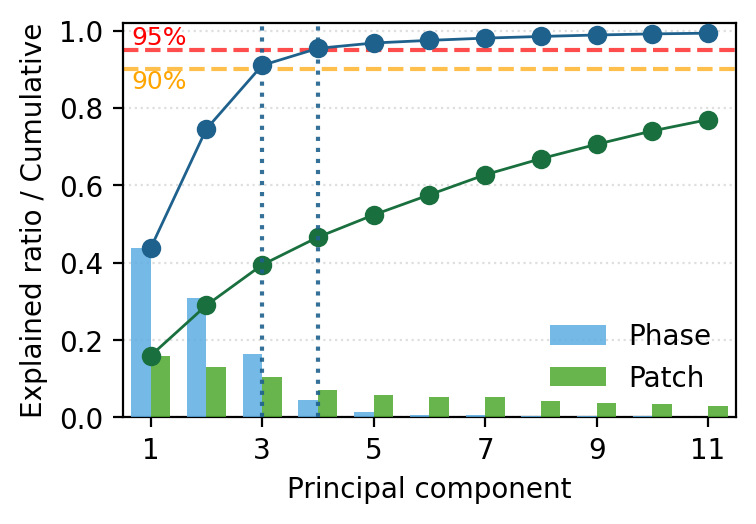
\includegraphics[width=\linewidth]{figures/etth1_pca_cycle_phase.png}
    \caption{PCA for tokens on \emph{ETTh1}.}
    \label{fig:pca_etth1}
  \end{subfigure}
  \hfill
  \begin{subfigure}[t]{0.32\textwidth}
    \centering
    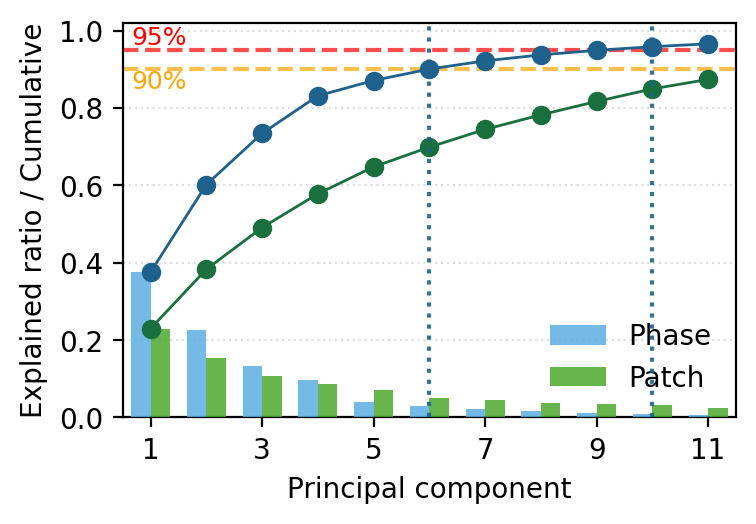
\includegraphics[width=\linewidth]{figures/etth2_pca_cycle_phase.png}
    \caption{PCA for tokens on \emph{ETTh2}.}
    \label{fig:pca_etth2}
  \end{subfigure}
  \hfill
  \begin{subfigure}[t]{0.32\textwidth}
    \centering
    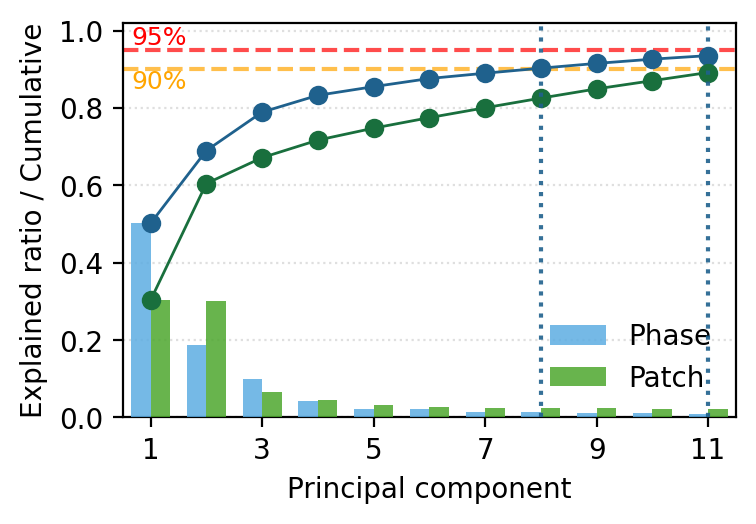
\includegraphics[width=\linewidth]{figures/ettm1_pca_cycle_phase.png}
    \caption{PCA for tokens on \emph{ETTm1}.}
    \label{fig:pca_ettm1}
  \end{subfigure}

  \vskip\baselineskip
  % 第二行
  \begin{subfigure}[t]{0.32\textwidth}
    \centering
    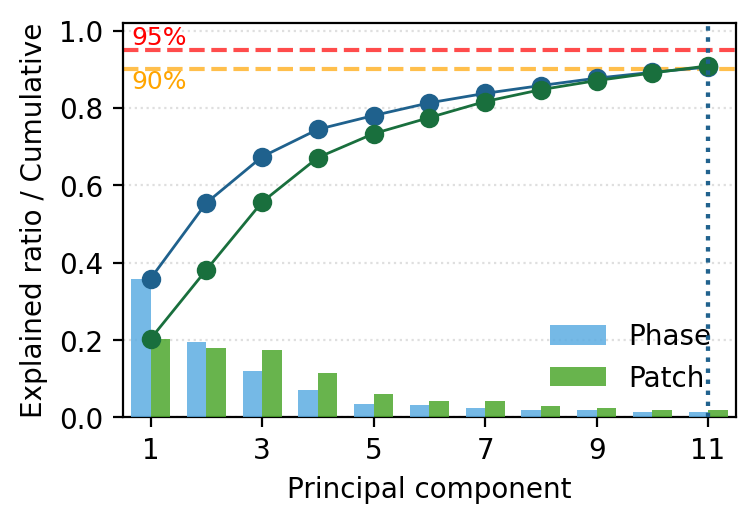
\includegraphics[width=\linewidth]{figures/ettm2_pca_cycle_phase.png}
    \caption{PCA for tokens on \emph{ETTm2}.}
    \label{fig:pca_ettm2}
  \end{subfigure}
  \hfill
  \begin{subfigure}[t]{0.32\textwidth}
    \centering
    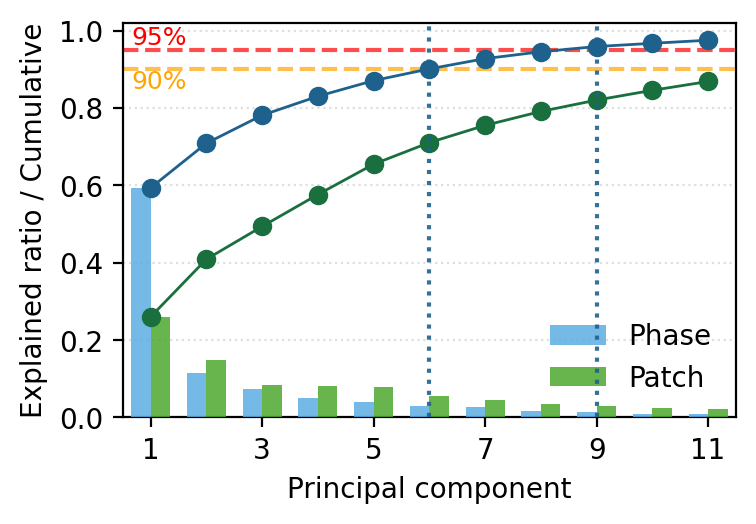
\includegraphics[width=\linewidth]{figures/electricity_pca_cycle_phase.png}
    \caption{PCA for tokens on \emph{Electricity}.}
    \label{fig:pca_ecl}
  \end{subfigure}
  \hfill
  \begin{subfigure}[t]{0.32\textwidth}
    \centering
    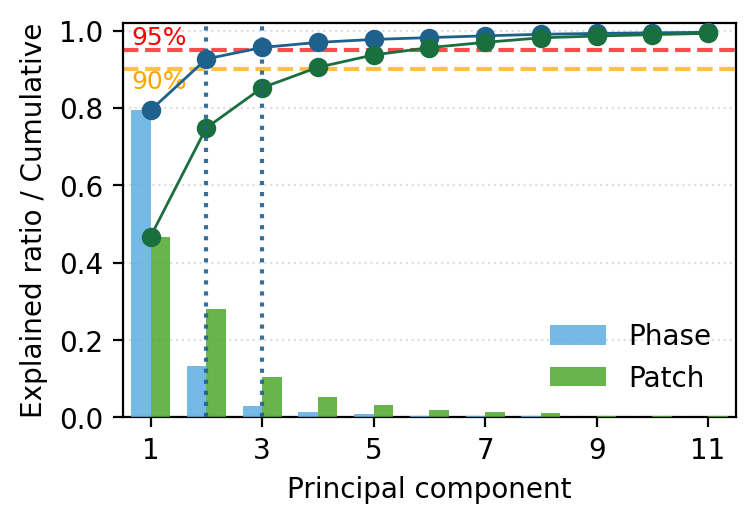
\includegraphics[width=\linewidth]{figures/weather_pca_cycle_phase.png}
    \caption{PCA for tokens on \emph{Weather}.}
    \label{fig:pca_weather}
  \end{subfigure}

  \caption{Visualization of phase tokenization across six datasets: ETTh1, ETTh2, ETTm1, ETTm2, Electricity, and Weather.}
  \label{fig:phase_token_comparison_detailed}
\end{figure*}

\revised{
\subsubsection{Comparison with Time Series Foundation Models}

To contextualize the performance of our approach, we compare \sysname against several representative foundation models drawn from the GIFT-Eval benchmark suite \citep{aksu2024giftevalbenchmarkgeneraltime}. 
Specifically, we include Chronos~\citep{ansari2024chronos}, Moirai~\citep{woo2024moirai}, and the recently released Moirai-2~\citep{liu2025moirai2} as baseline models.

Due to space limitations, we report results on the Web/DevOps subsets of the benchmark in \tabref{tab:model_mse_comparison}. 
These Web/DevOps datasets are \textit{not} well-studied by many existing works~\citep{nie2023patchtst, zhang2023crossformer, huang2025timebase, fits2024, lin2024sparsetsf}. 
Their heterogeneous and highly non-stationary behaviors make them particularly challenging, and thus provide a realistic environment to evaluate the generalization capability of large time series foundation models.

Beyond demonstrating strong overall competitiveness, the empirical results clearly highlight the 
unique strengths of phase-based representation in handling 
\emph{high-variance, noise-heavy workload patterns}. 
In particular, \sysname consistently outperforms all foundation-model baselines on the \texttt{bitbrains\_rnd} and \texttt{bitbrains\_fast\_storage} datasets—-two challenging subsets in GIFT-Eval due to frequent spikes and abrupt intensity shifts.
These results indicate that \sysname's phase-aware design provides substantially improved robustness and stability under highly volatile real-world workload traces, where traditional architecture tend to degrade.
}

\revised{
\begin{table*}[t]
\centering
\caption{Comparison of MSE (Mean) Across Four Forecasting Models on Web/CloudOps Datasets provided in GIFT-Eval.}
\label{tab:model_mse_comparison}
\footnotesize
\begin{tabular}{lcccc|c}
\hline
\textbf{Dataset} & \textbf{\sysname} & \textbf{Moirai-2} & \textbf{Moirai-base} & \textbf{Chronos-base} & \textbf{Best Model} \\
\hline
bizitobs\_l2c/5T/short           & 39.4347      & \textbf{20.6240}   & 22.1000        & 24.1000        & Moirai-2 \\
bizitobs\_l2c/H/short            & 99.9582      & \textbf{67.8501}   & 272.0000       & 243.0000       & Moirai-2 \\
bitbrains\_rnd/H/short           & \textbf{1,970,330} & 2,235,573     & 4,020,000      & 2,210,000      & \sysname \\
bitbrains\_rnd/5T/short          & \textbf{1,606,034} & 1,660,532     & 180,000,000    & 1,800,000      & \sysname \\
bizitobs\_application/10S/short  & 4,653,132    & \textbf{621,852}   & 6,360,000      & 6,030,000      & Moirai-2 \\
bitbrains\_fast\_storage/H/short & \textbf{2,585,180}    & 2,942,651          & 604,000,000    & 2,620,000 & \sysname \\
bitbrains\_fast\_storage/5T/short& \textbf{1,887,398} & 2,142,125     & 25,400,000,000 & 1,920,000      & \sysname \\
bizitobs\_service/10S/short      & 26,523       & \textbf{4,798}     & 51,900         & 37,100         & Moirai-2 \\
\hline
\end{tabular}
\end{table*}
}




\subsection{Additional Hyper Parameters Analysis}
\subsubsection{Impact of Model Parameter Scale on Performance}
We conducted comparative experiments on three variants of the \sysname model with different parameter scales across the Electricity, Traffic, and Weather datasets. The three configurations are: a single-layer model with latent dimension 8 ($\approx$1.72K parameters), a single-layer model with latent dimension 16 ($\approx$5.48K parameters), and a two-layer model with latent dimension 32 ($\approx$37.1K parameters). \figref{tab:phaseformer_params_variants} summarizes the results in terms of MSE, MAE and FLOPs.

Overall, the effect of model scale on performance is not consistent. On the Traffic dataset, larger models yield slight improvements, whereas on the Electricity and Weather datasets, the smaller and medium-sized models perform better. These findings indicate that \sysname achieves a favorable balance between computational efficiency and predictive accuracy at relatively small parameter scales, and increasing model size does not lead to uniform gains across all tasks.

\begin{table*}[t]
\centering
\caption{Comparison of \sysname variants. Each cell reports MSE, MAE, and FLOPs. The input length is fixed as 720 steps and the output length is fixed as 96 steps. The best results are marked with \best{Bold}, and the second-best results are marked with \second{Underlined}.}
\label{tab:phaseformer_params_variants}
\small  % 或者 \footnotesize, \scriptsize
\begin{tabular}{c|ccc|ccc|ccc}
\hline
\multirow{2}{*}{Dataset}
& \multicolumn{3}{c|}{\textbf{\sysname-1.7K}} 
& \multicolumn{3}{c|}{\textbf{\sysname-5K}} 
& \multicolumn{3}{c}{\textbf{\sysname-37K}} \\
\cline{2-10}
& MSE & MAE & FLOPs
& MSE & MAE & FLOPs
& MSE & MAE & FLOPs \\
\hline
Electricity 
& \best{0.129} & \best{0.220} & \best{9.41M}
& \best{0.129} & \second{0.221} & \second{31.97M}
& \second{0.131} & \second{0.223} & 221.05M \\
Traffic     
& \second{0.361} & \second{0.241} & \best{25.27M}
& 0.366 & 0.243 & \second{85.84M}
& \best{0.360} & \best{0.236} & 593.61M \\
Weather     
& \best{0.150} & \second{0.199} & \best{0.62M}
& \second{0.151} & \best{0.194} & \second{2.09M}
& 0.174 & 0.217 & 14.46M \\
\hline
\end{tabular}
\end{table*}

\subsubsection{Impact of Input Length on Performance}

We examine how the input window size affects the prediction accuracy and computational cost of \sysname. 
Throughout this section, $L$ denotes using the most recent $L$ time steps as model input. The output length is fixed as 96 steps.
As summarized in ~\figref{fig:input_length_prediction_errors}, increasing $L$ reduces MSE and MAE across datasets, indicating that \sysname benefits from longer historical context for modeling long-range temporal dependencies.

In terms of efficiency, the parameter count and FLOPs per forward pass remain nearly constant as $L$ increases, with only modest growth (see ~\figref{fig:input_length_efficiency}) attributable primarily to the embedding stage. 
This behavior arises because the sequence length processed by the core encoder/decoder is governed by the number of \emph{phases}, which depends on the data’s learned periodic structure rather than by the raw input length.
Consequently, scaling $L$ mainly affects the embedding computations, whose cost is relatively small compared to the phase-based modules.

\begin{figure*}[htbp]
    \centering
    % 子图1: Electricity
    \begin{subfigure}[b]{0.32\textwidth}
        \centering
        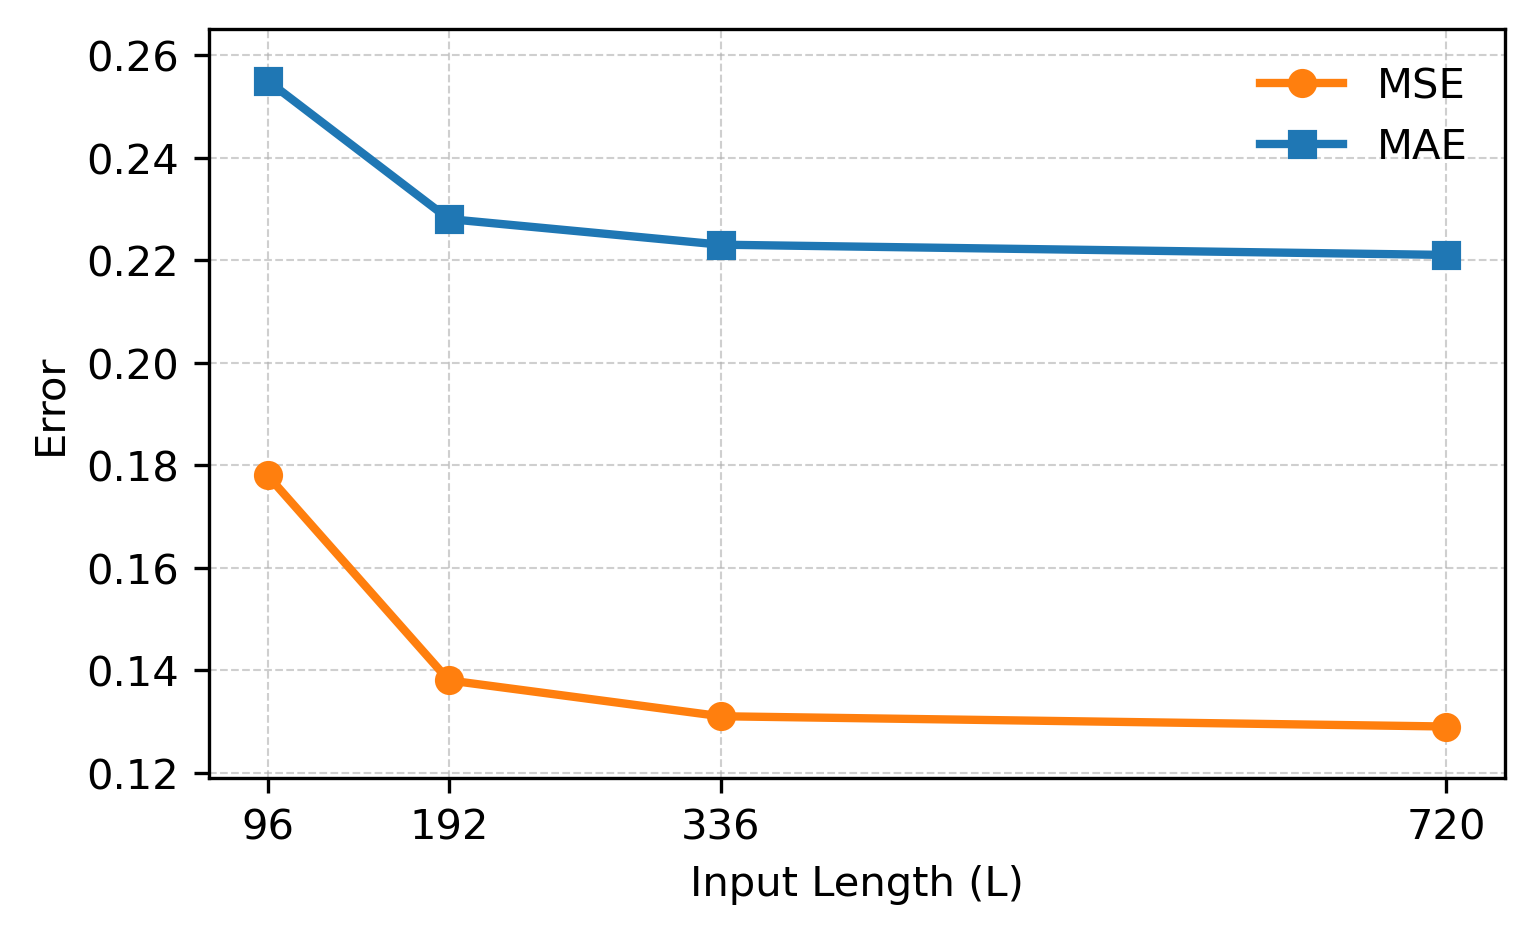
\includegraphics[width=\textwidth]{figures/performance_electricity.png}
        \caption{Electricity}
    \end{subfigure}
    % 子图2: Traffic
    \begin{subfigure}[b]{0.32\textwidth}
        \centering
        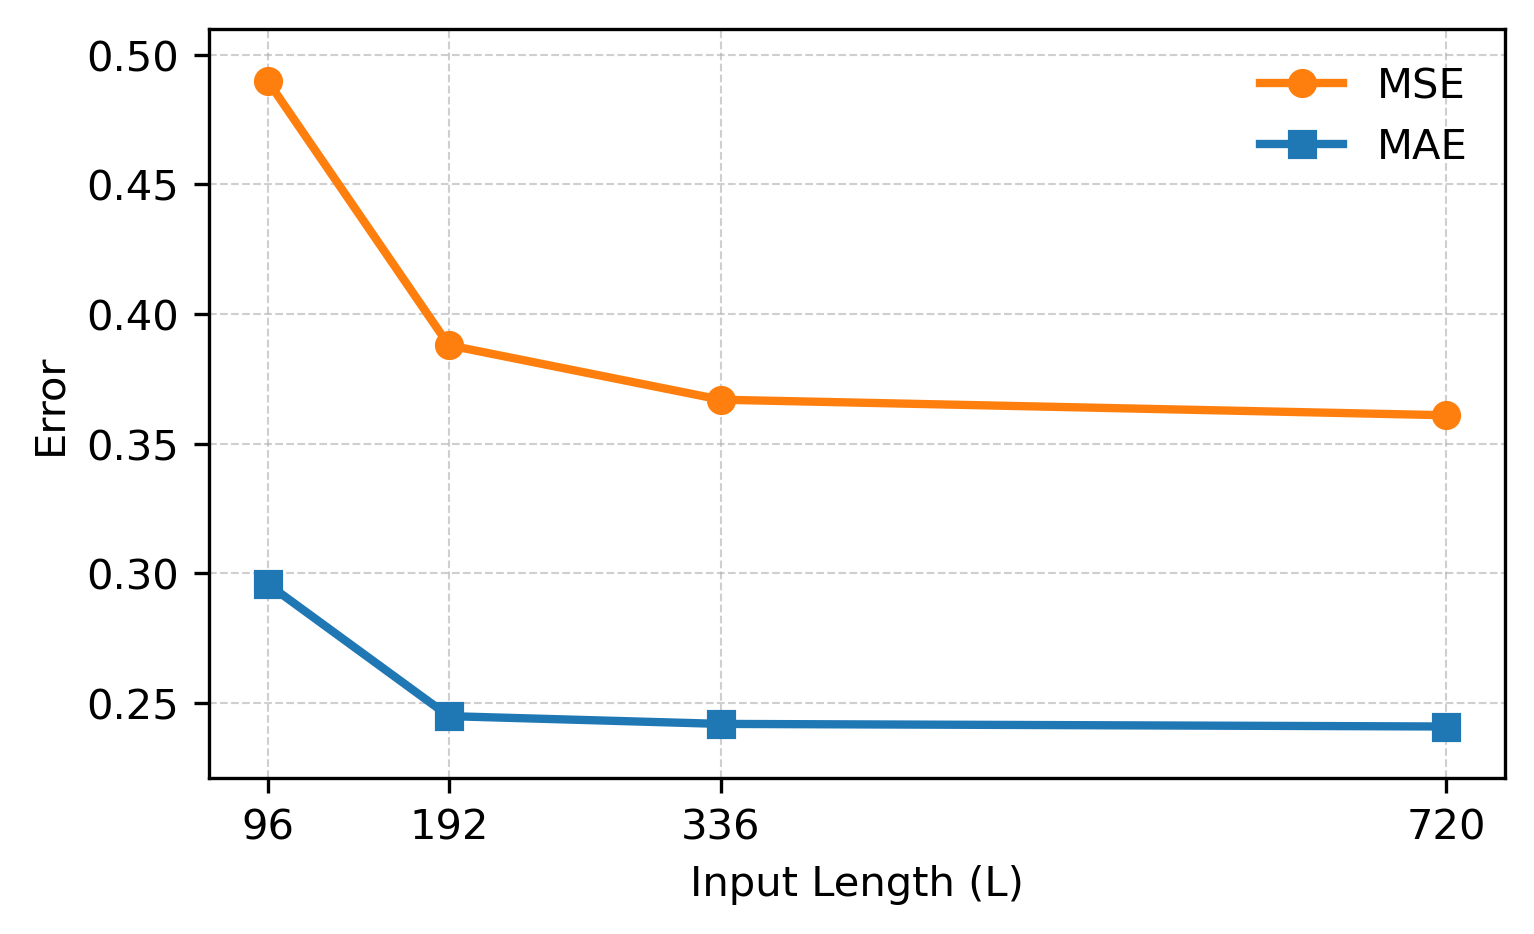
\includegraphics[width=\textwidth]{figures/performance_traffic.png}
        \caption{Traffic}
    \end{subfigure}
    % 子图3: Weather
    \begin{subfigure}[b]{0.32\textwidth}
        \centering
        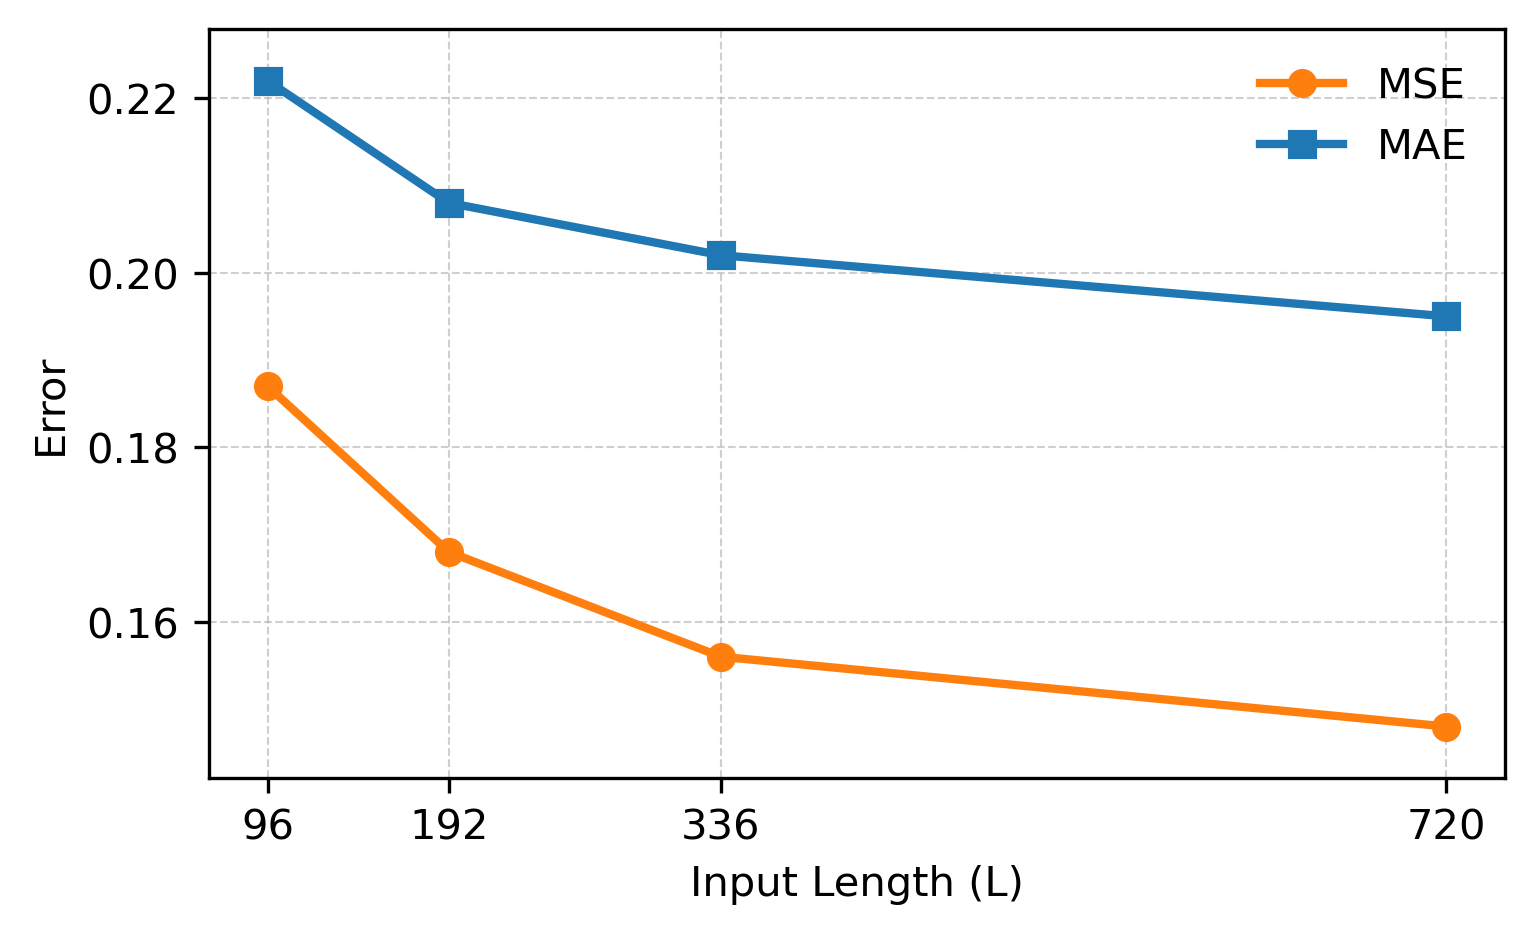
\includegraphics[width=\textwidth]{figures/performance_weather.png}
        \caption{Weather}
    \end{subfigure}

    \caption{Prediction error test results across datasets under different input lengths.}
    \label{fig:input_length_prediction_errors}
\end{figure*}

\begin{figure*}[htbp]
    \centering
    % 子图1: Electricity
    \begin{subfigure}[b]{0.32\textwidth}
        \centering
        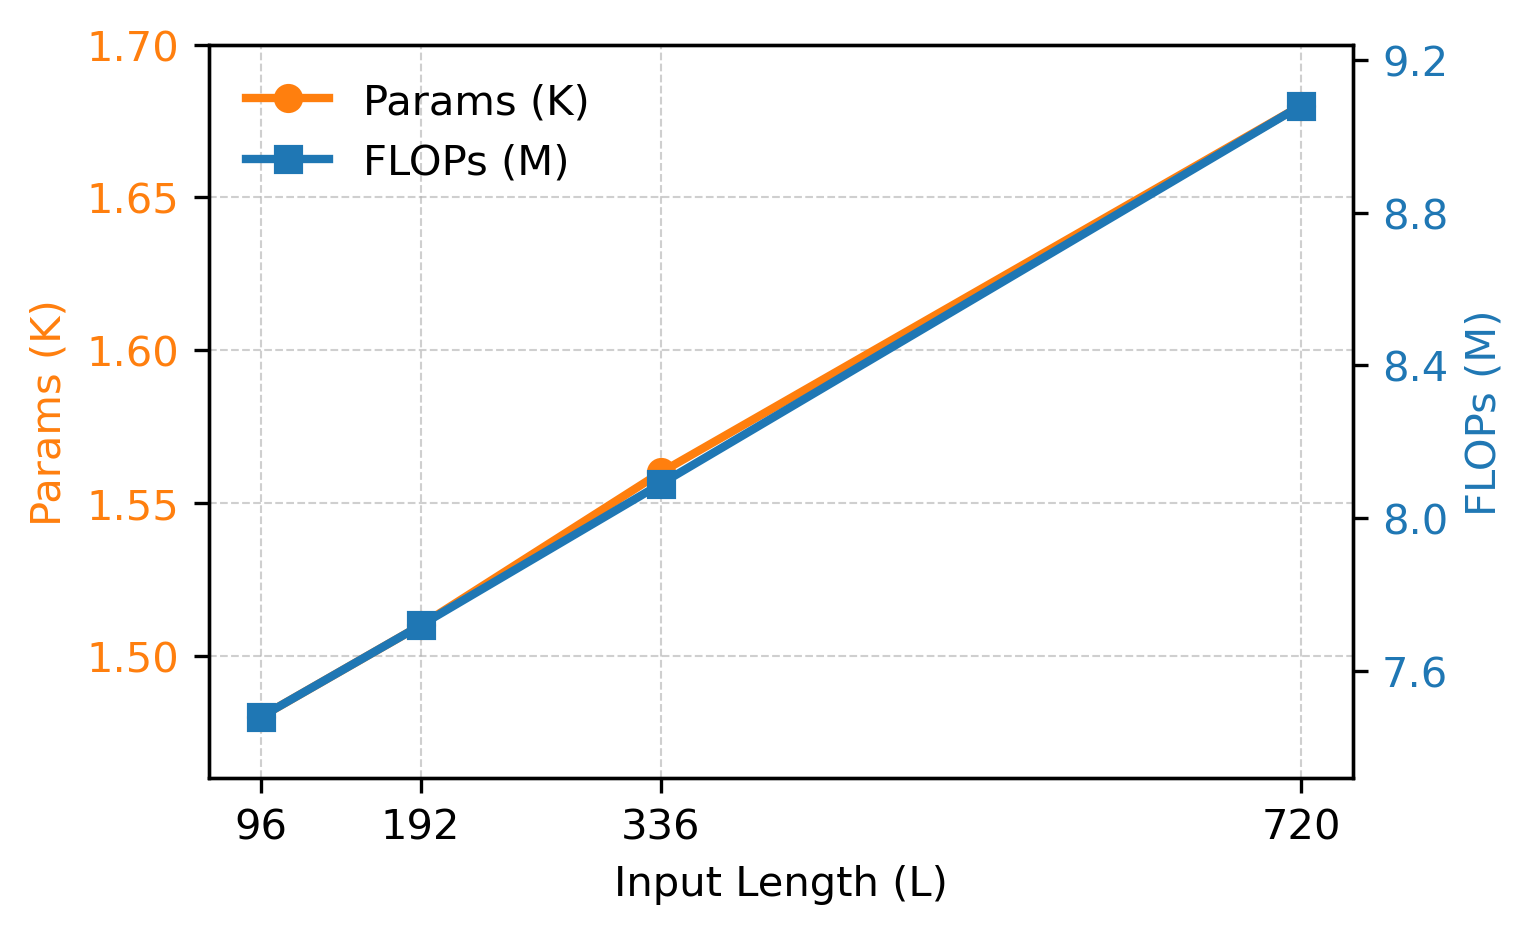
\includegraphics[width=\textwidth]{figures/efficiency_electricity.png}
        \caption{Electricity}
    \end{subfigure}
    % 子图2: Traffic
    \begin{subfigure}[b]{0.32\textwidth}
        \centering
        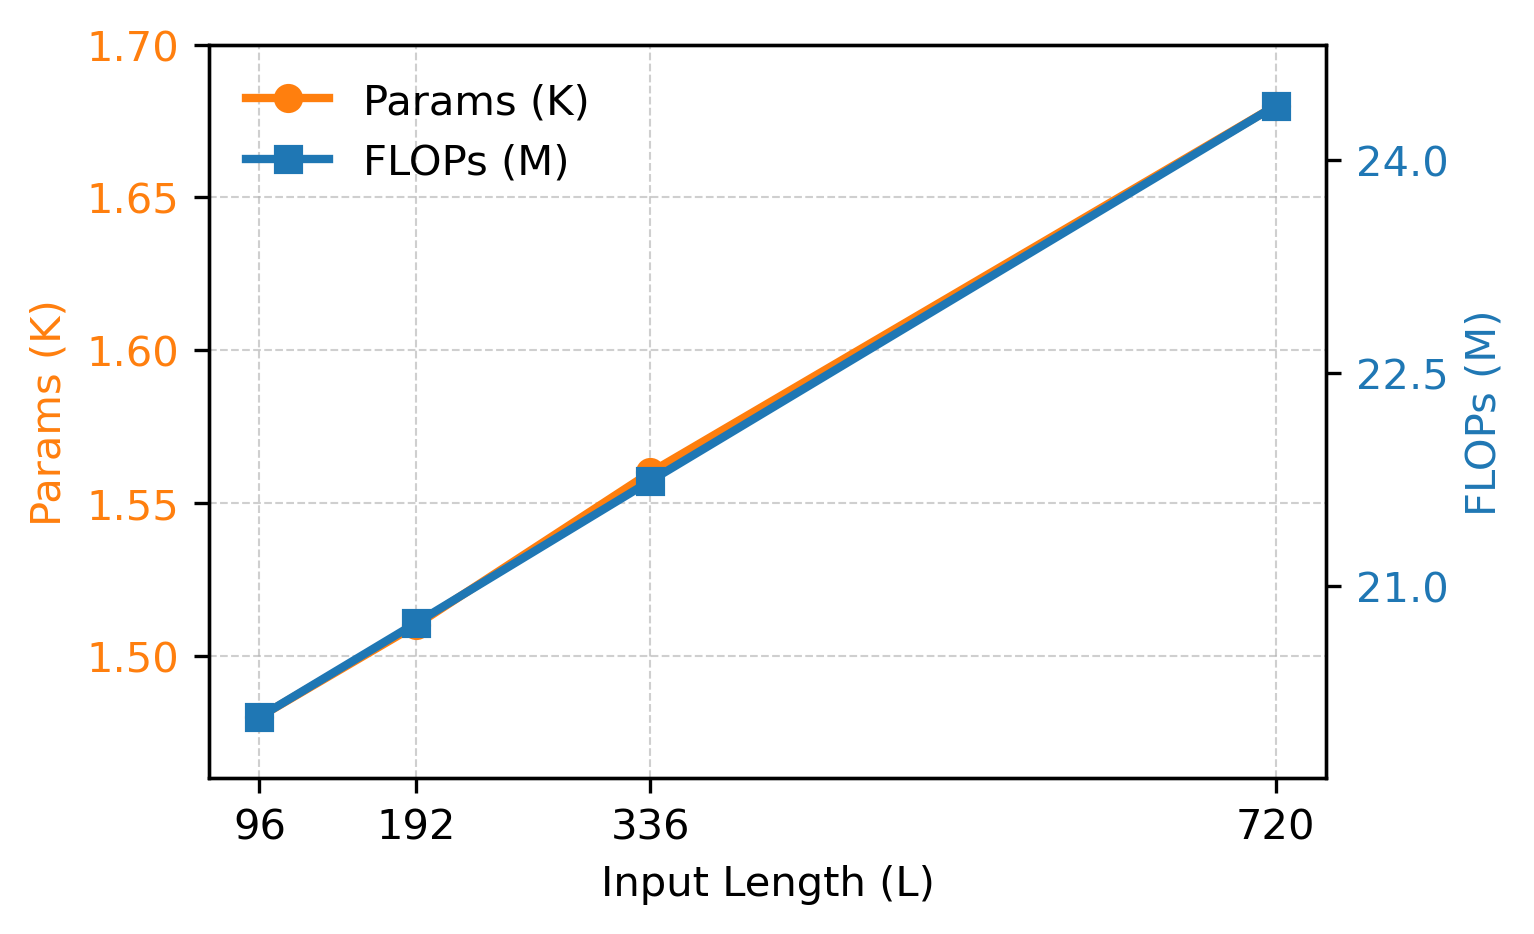
\includegraphics[width=\textwidth]{figures/efficiency_traffic.png}
        \caption{Traffic}
    \end{subfigure}
    % 子图3: Weather
    \begin{subfigure}[b]{0.32\textwidth}
        \centering
        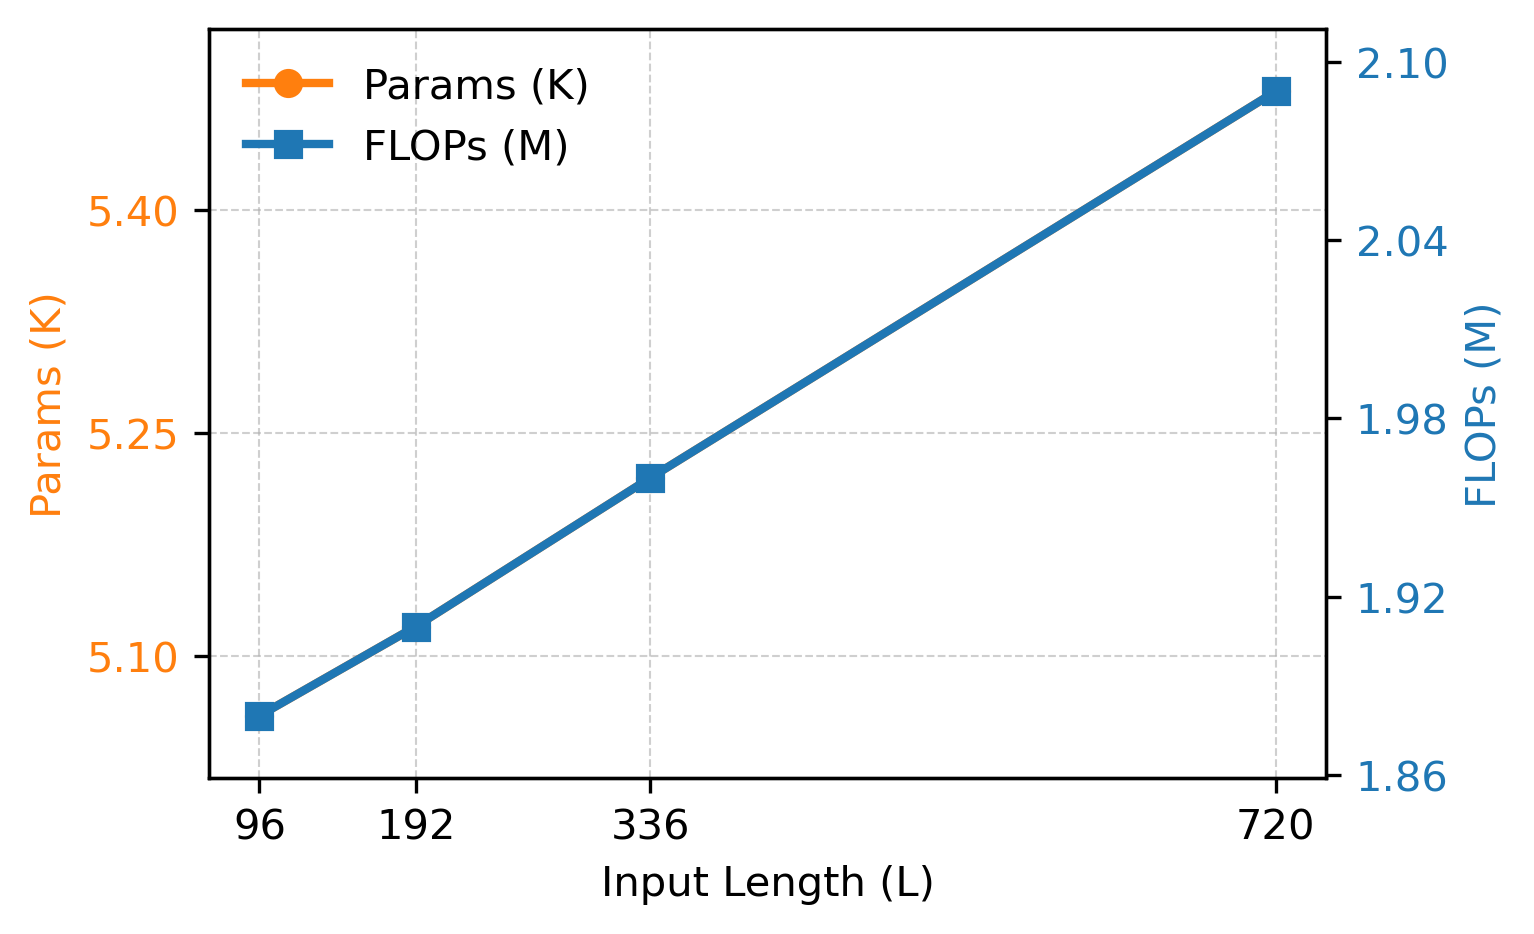
\includegraphics[width=\textwidth]{figures/efficiency_weather.png}
        \caption{Weather}
    \end{subfigure}

    \caption{Efficiency evaluation of \sysname\ across datasets with varying input lengths.}
    \label{fig:input_length_efficiency}
\end{figure*}

\revised{
\subsection{Analysis of Fine-Grained Temporal Information Retention}
To examine whether Phase Tokenization preserves essential intra-cycle dynamics after compressing periodic structures, we conduct a reconstruction experiment on the Traffic dataset. Given an input sequence of length 720, \sysname is trained to reconstruct sequences of the same length, removing forecasting uncertainty and isolating the representational capacity of the phase embeddings.

\fakeparagraph{Setup}
We evaluate the retention of fine-grained information by computing the reconstruction residual and analyzing it in both the time and frequency domains. In particular, we estimate the power spectral density (PSD) of the residual to detect whether certain frequency components, especially those associated with short-term or high-frequency dynamics, are systematically diminished.

\begin{figure*}
    \centering
    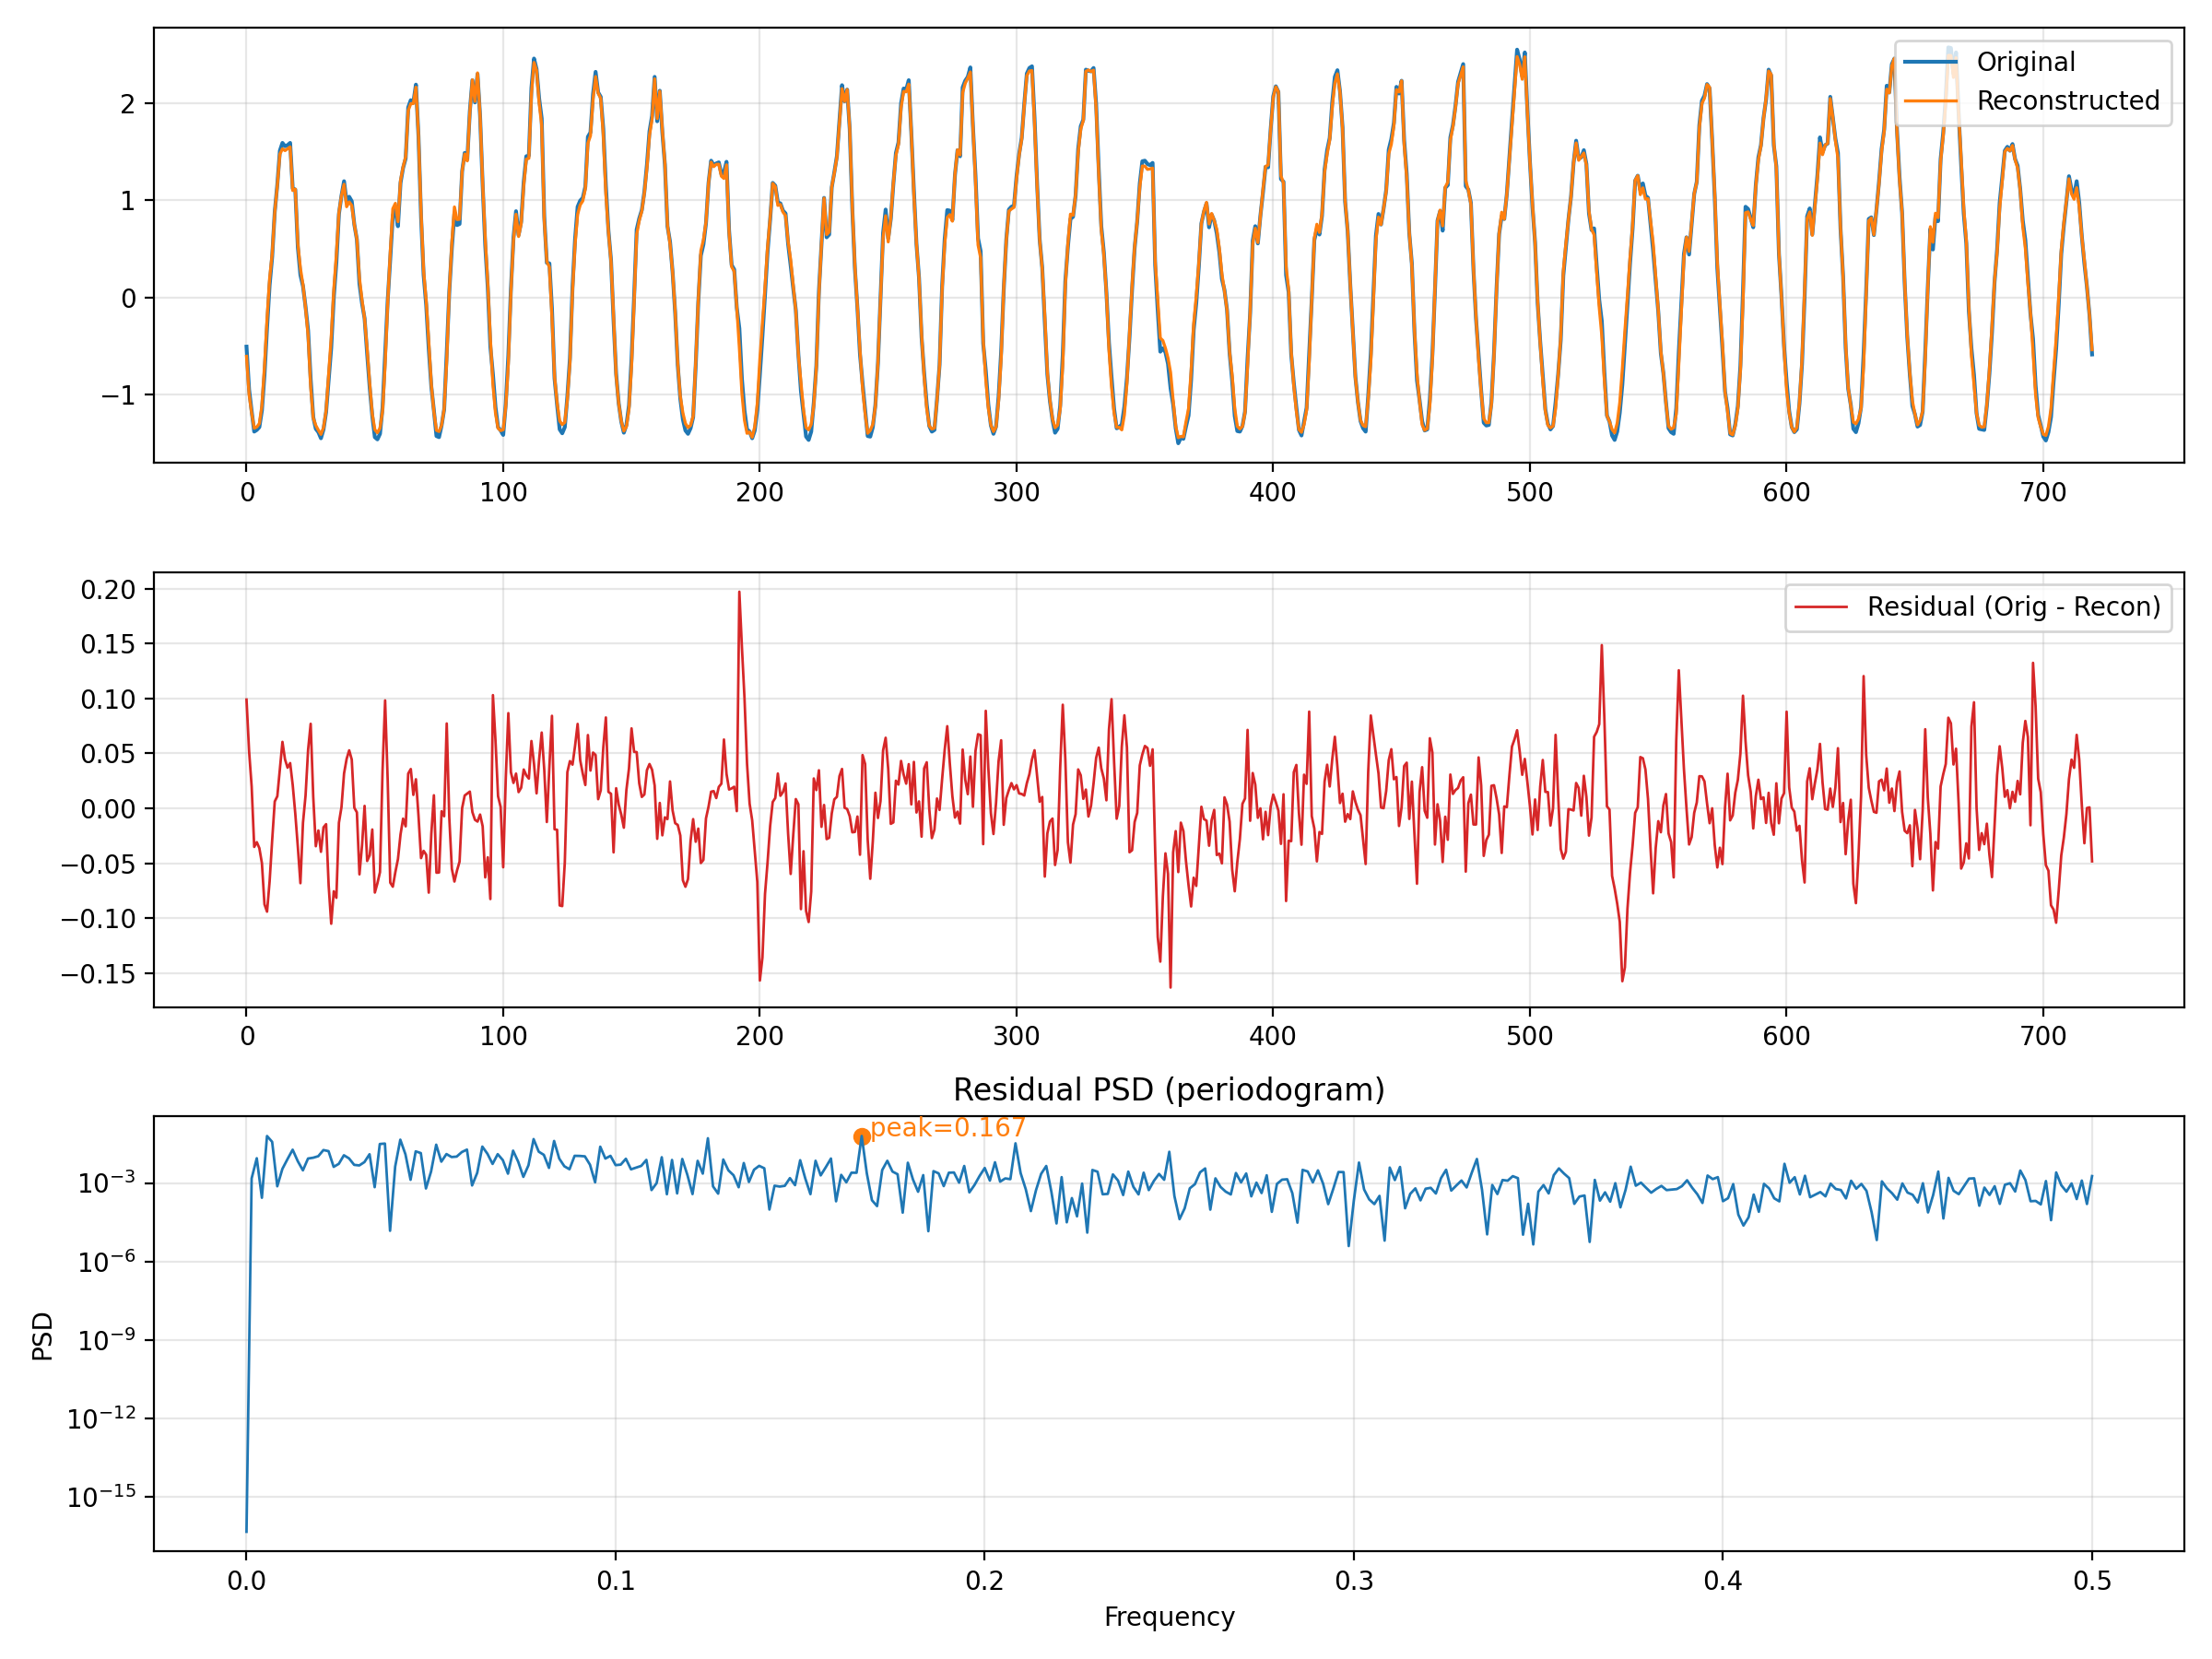
\includegraphics[width=0.75\textwidth]{figures/reconstruction_analysis.png}
    \caption{Time-domain and power-spectrum visualizations of the reconstruction residuals when \sysname reconstructs 720 input time steps on the Traffic dataset.}
    \label{fig:reconstruction_analysis}
\end{figure*}

\fakeparagraph{Frequency Analysis of the Residual}
The PSD analysis in \figref{fig:reconstruction_analysis} shows that residual energy is evenly distributed across the spectrum, with no noticeable concentration or suppression in any frequency band. This indicates that Phase Tokenization does not introduce frequency-dependent information loss. Despite compressing each cycle into a compact phase representation, the model retains the ability to capture fine-grained intra-cycle dynamics, supporting the effectiveness of phase-based temporal abstraction for long-sequence forecasting.
}



\subsection{Showcases}

To provide a clearer comparison of predictive performance across different models, we present the results of \sysname, PatchTST, FITS, and TimeBase on the Traffic dataset.
\sysname demonstrates strong predictive performance, as reflected by both the shape of its forecasts and the actual prediction errors.

Compared with \sysname, PatchTST produces lower peak values within each cycle, failing to fully match the true curve. This discrepancy is likely due to phase shifts in the periodic pattern that reduce peak amplitudes.
FITS, which performs prediction in the frequency domain with frequency band partitioning, tends to overlook high-frequency information. As a result, its predictions deviate from the ground truth, though the forecasts still preserve a periodic structure.
TimeBase aligns well with the general cyclical pattern but fails to capture true variations across cycles, a limitation stemming from its patch-based basis construction mechanism.


\begin{figure*}[t]
    \centering
    % 第一行
    \begin{subfigure}{0.47\textwidth}
        \centering
        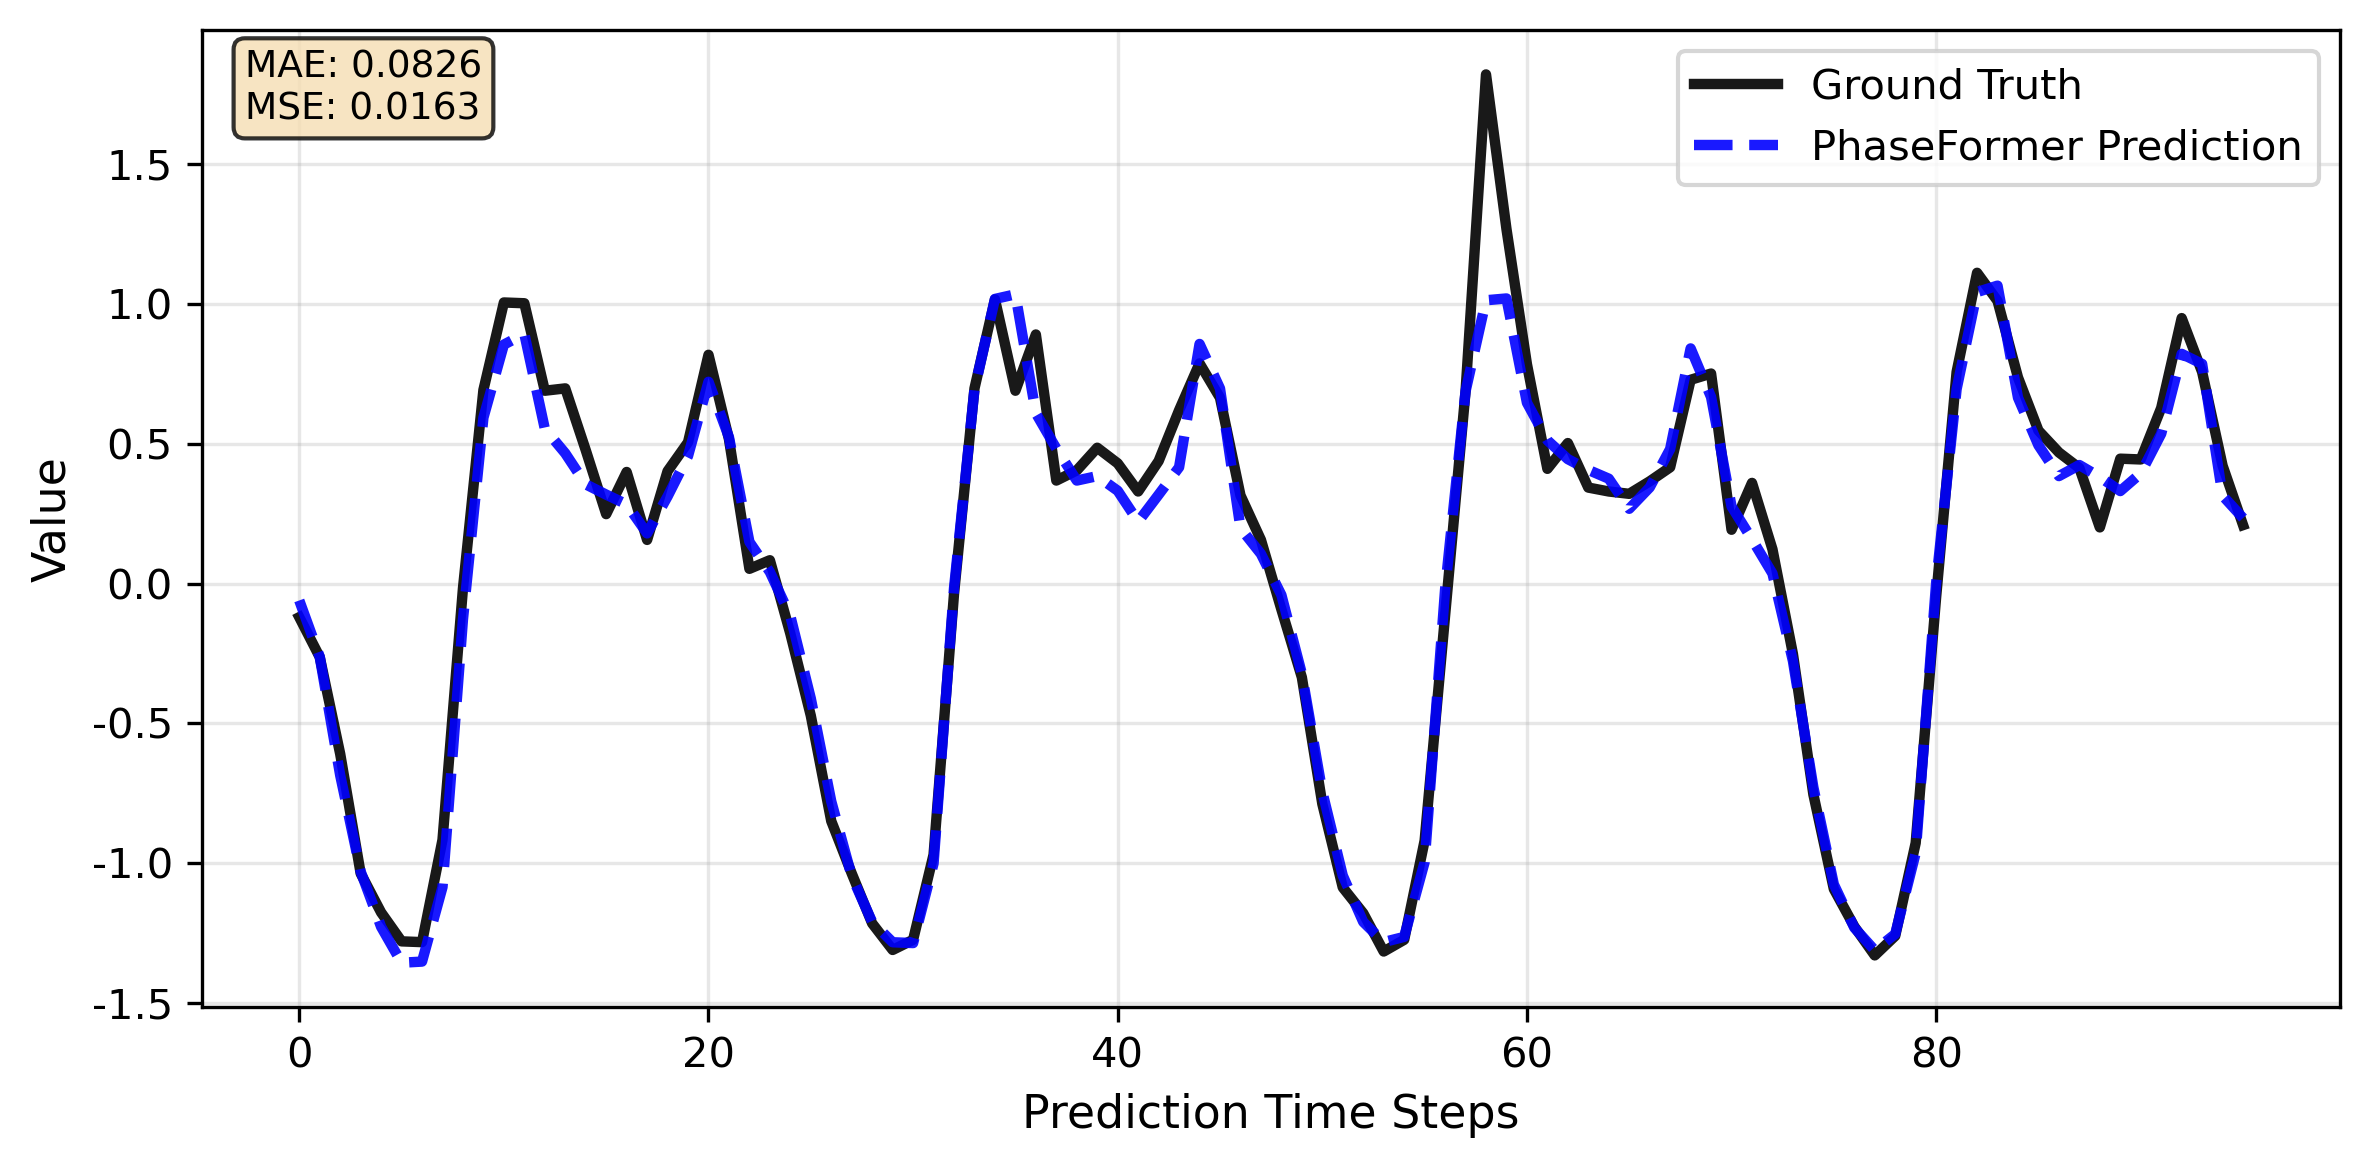
\includegraphics[width=\linewidth]{figures/PhaseFormer_prediction_20250923_021323.png}
        \caption{\sysname}
    \end{subfigure}
    \hfill
    \begin{subfigure}{0.47\textwidth}
        \centering
        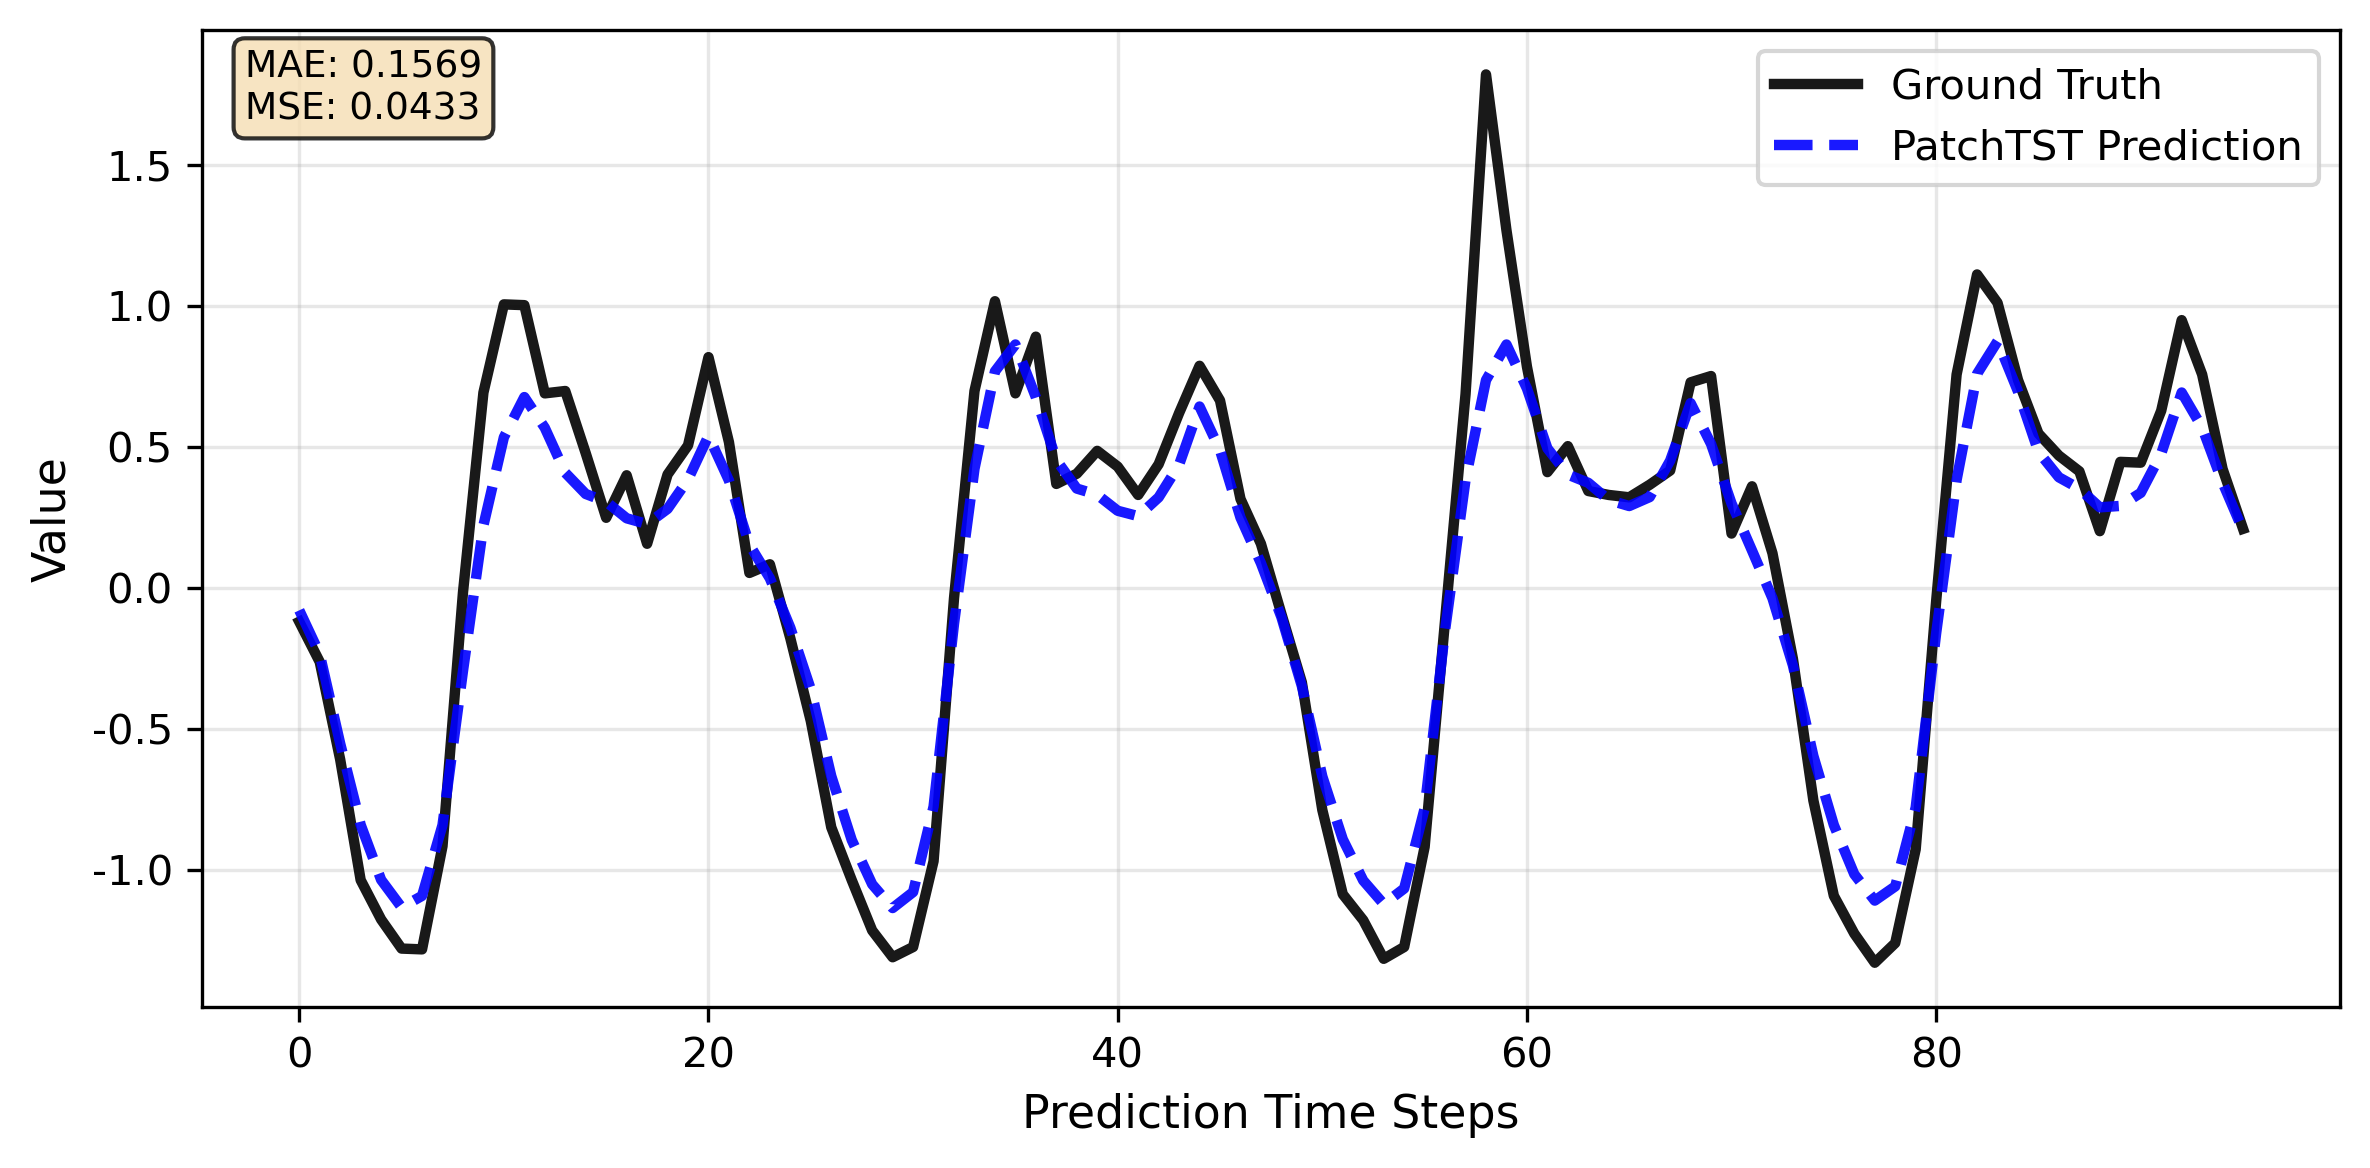
\includegraphics[width=\linewidth]{figures/PatchTST_prediction_20250923_021323.png}
        \caption{PatchTST}
    \end{subfigure}

    % 第二行
    \vskip\baselineskip
    \begin{subfigure}{0.47\textwidth}
        \centering
        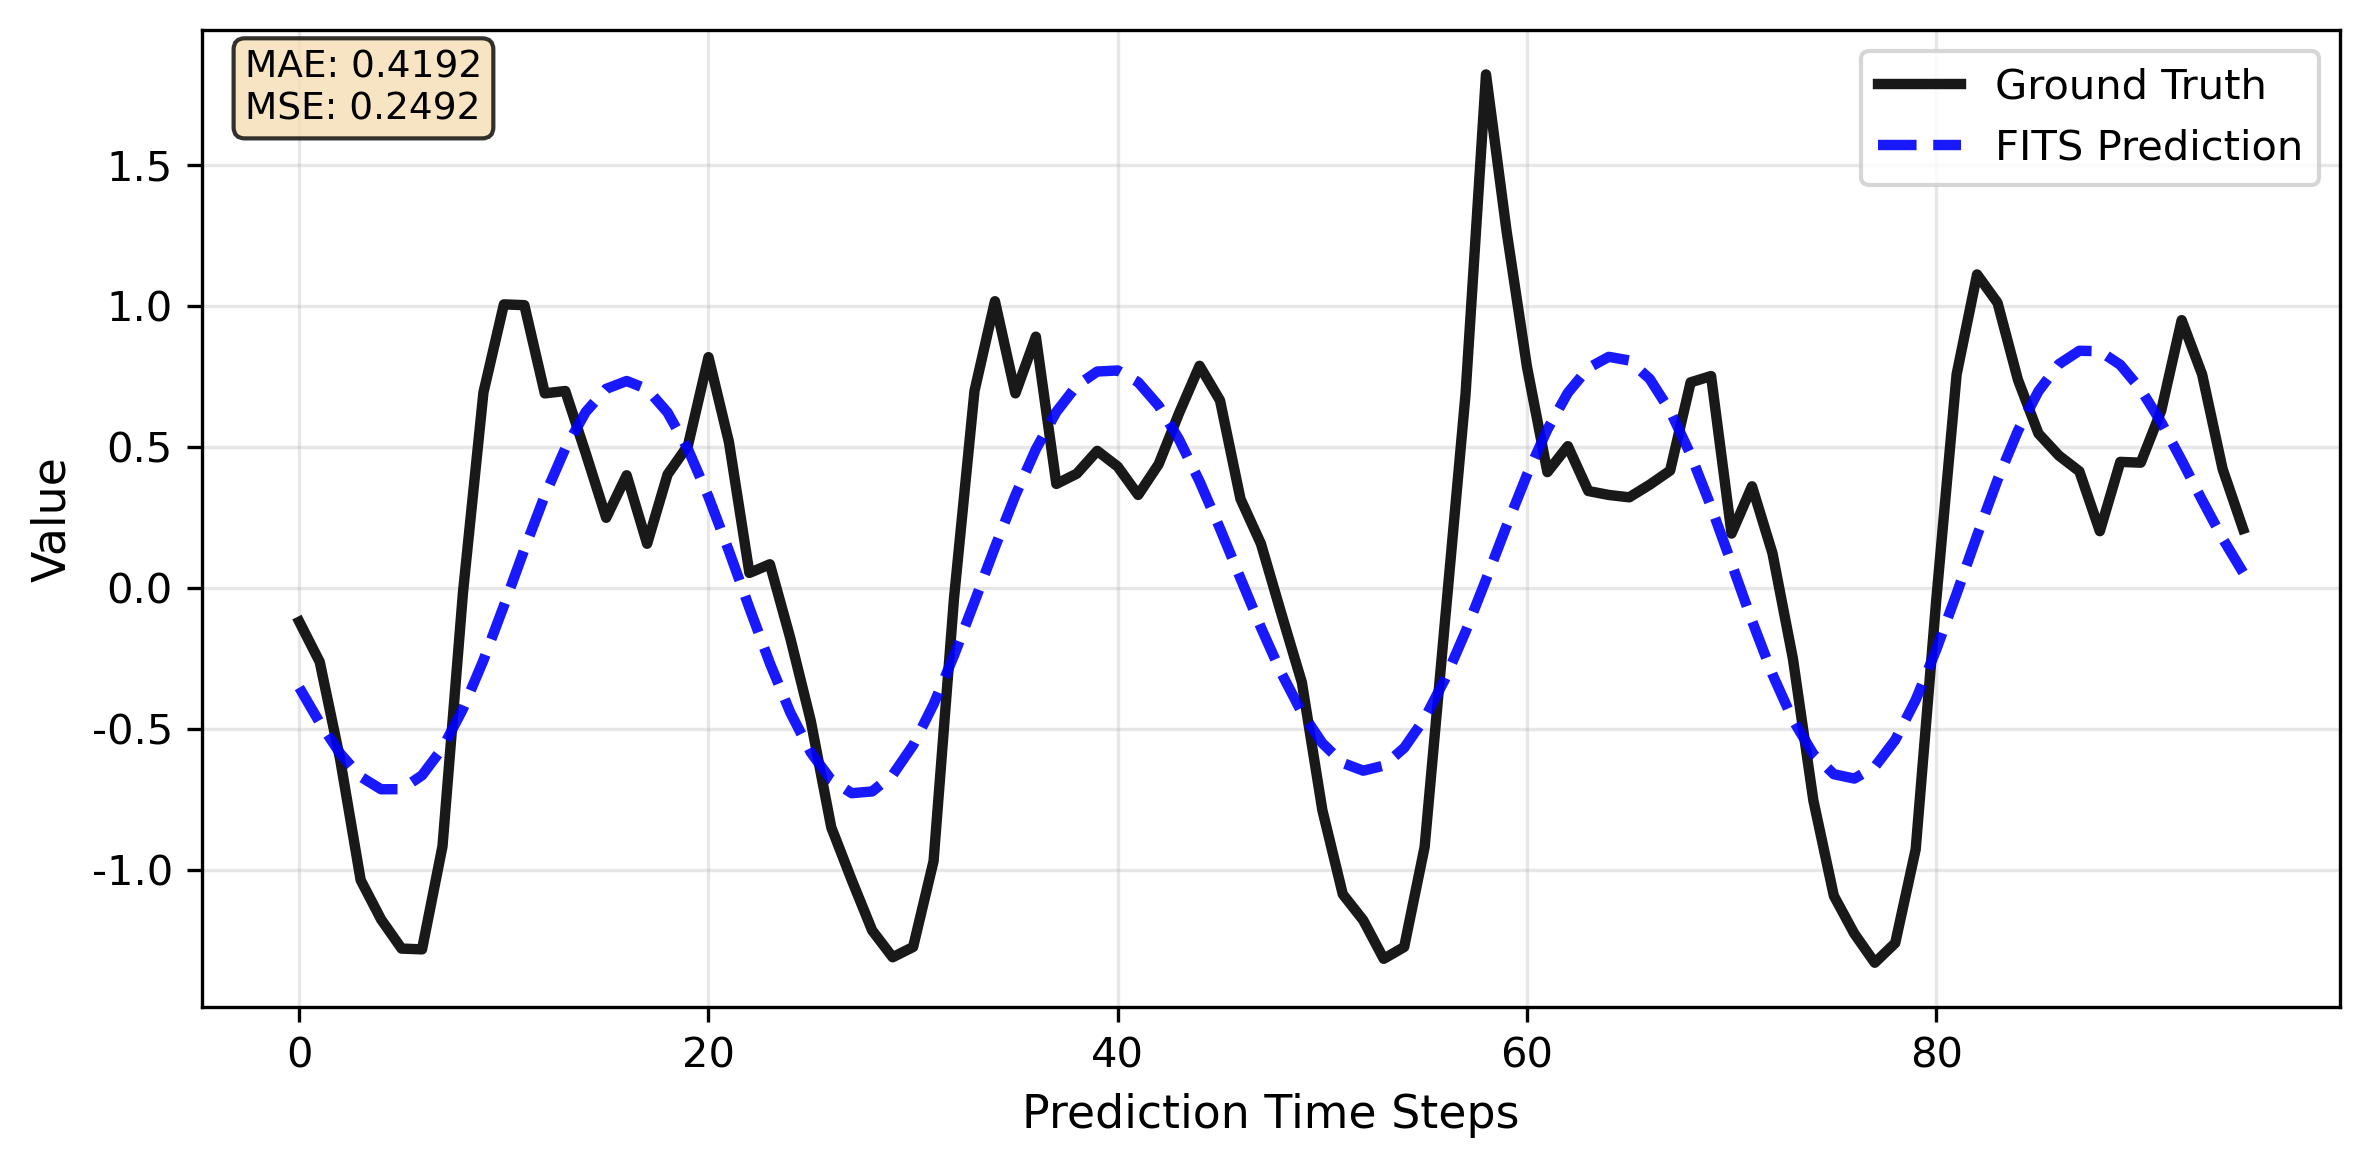
\includegraphics[width=\linewidth]{figures/FITS_prediction_20250923_021323.png}
        \caption{FITS}
    \end{subfigure}
    \hfill
    \begin{subfigure}{0.47\textwidth}
        \centering
        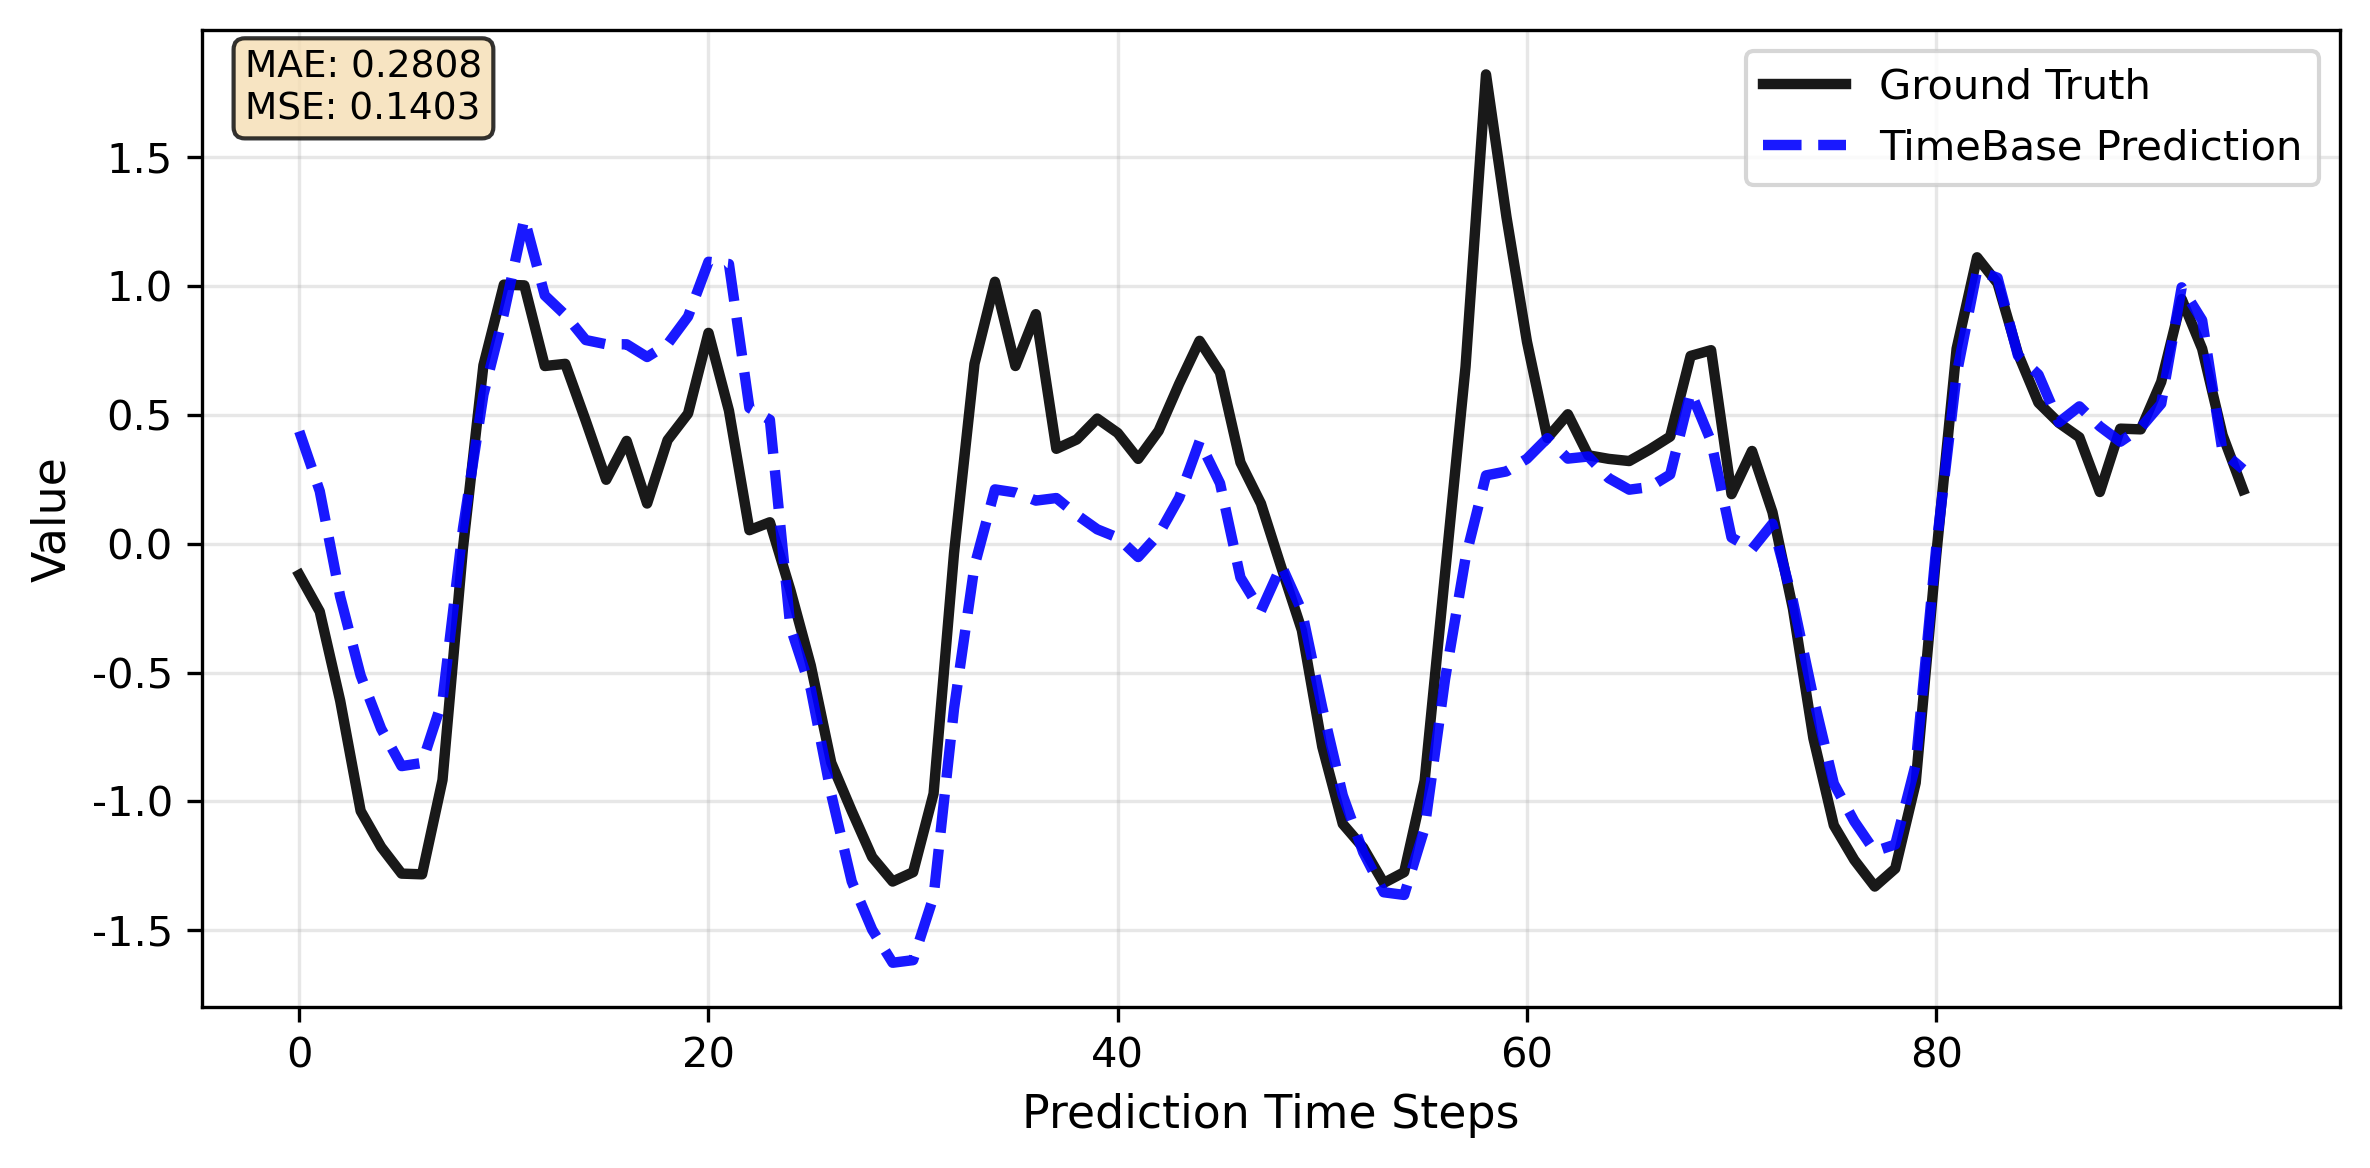
\includegraphics[width=\linewidth]{figures/TimeBase_prediction_20250923_021323.png}
        \caption{TimeBase}
    \end{subfigure}

    \caption{Visualization of forecasting results on Traffic dataset. The black lines stand for the ground truth and the \textcolor{blue}{blue} lines stand for forecasting results.}
\end{figure*}


\subsection{Theoretical Analysis for Phase Tokenization}
\label{sub:theoretical}
\revised{
Under the classical finite-order linear system assumption, the structural dependencies in a time series (especially periodic or quasi-periodic components) are reflected in the rank properties of suitable delay-embedding matrices.

Consider a univariate time series
\[
x_1, x_2, \ldots, x_T.
\]
Fix a collection of delays (lags) \(\tau_1,\ldots,\tau_D\) and a set of reference indices \(s_1,\ldots,s_H\) such that
\(s_h + \tau_D \le T\) for all \(h\).
The corresponding \(D \times H\) delay-embedding matrix is
\[
X =
\begin{bmatrix}
x_{s_1+\tau_1} & x_{s_2+\tau_1} & \cdots & x_{s_H+\tau_1} \\
x_{s_1+\tau_2} & x_{s_2+\tau_2} & \cdots & x_{s_H+\tau_2} \\
\vdots & \vdots &        & \vdots \\
x_{s_1+\tau_D} & x_{s_2+\tau_D} & \cdots & x_{s_H+\tau_D}
\end{bmatrix}.
\]
The classical Hankel matrix is recovered as the special case with unit delay and consecutive indices, e.g.\ \(\tau_d=d-1\) and \(s_h=h\), but our analysis does not rely on this specific structure.

If the series is dominated by periodic or harmonic components, it can often be generated (or well approximated) by a low-dimensional linear dynamical system. In this case, the delay-embedding matrix \(X\) exhibits a natural \textbf{low-rank} structure: its columns lie approximately in a low-dimensional subspace determined by the underlying system dynamics. Only when the series resembles unstructured white noise does the delay-embedding matrix approach full rank.

For a univariate periodic (or quasi-periodic) series, such a delay-embedding admits the factorization
\[
X = A G,
\]
where \(A\) and \(G\) encode, respectively, the delay-dependent responses and the coefficients associated with different reference indices (e.g., days or windows). The parameters \(D\), the choice of delays \(\{\tau_d\}\), and the number of columns \(H\) jointly determine the shape of the embedding.

Thus, we model the data matrix as
\[
X \;=\; A G^\top + N \;\in\;\mathbb{R}^{D\times H},
\]
}
where $A\in\mathbb{R}^{D\times r}$, $G\in\mathbb{R}^{H\times r}$ are column full rank with $\operatorname{rank}(A)=\operatorname{rank}(G)=r$, and $N$ is noise. The true signal is $M = A G^\top$. We assume $r\ll \min(D,H)$.

Patch tokenization corresponds to the row space $\mathrm{Row}(X)$ (the right singular $r$-subspace), while phase tokenization corresponds to the column space $\mathrm{Col}(X)$ (the left singular $r$-subspace).

A shared transformation applies $S\in\mathbb{R}^{H\times H}$ on the hourly dimension:
\[
\blue{X^{\prime}} = X S^\top = A (S G)^\top + \blue{N^{\prime}}.
\]

\revised{
In our formulation, the set $S$ represents a family of linear transformations applied to the input sequence. 
Such transformations frequently arise in practical systems due to sensor delays, timing jitters, or preprocessing procedures including smoothing or temporal alignment.

}

For a matrix $Y$, define the spectral separation as
\[
\mathrm{sep}_r(Y) := \min_{i\le r,\,j>r}|\sigma_i(Y)-\sigma_j(Y)|.
\]
When $\operatorname{rank}(Y)=r$, this equals $\sigma_r(Y)$. In particular,
\[
\delta = \sigma_r(M), \quad \delta'=\sigma_r(MS^\top), \quad
\delta_{\min}=\min(\delta,\delta').
\]
Assume $S$ is invertible on $\mathrm{Col}(G)$, i.e. $\operatorname{rank}(S G)=r$. Define
\[
\kappa := \sigma_{\min}(S|_{\mathrm{Col}(G)})>0.
\]
Moreover, since $\sigma_r(M)\ge\sigma_r(A)\sigma_r(G)$ and 
$\sigma_r(MS^\top)\ge \kappa\sigma_r(A)\sigma_r(G)$, we have the useful bound
\[
\delta_{\min}\;\ge\;\min(1,\kappa)\,\sigma_r(A)\sigma_r(G).
\]

For two $r$-dimensional subspaces $\mathcal U,\mathcal V$, their distance is
\[
d(\mathcal U,\mathcal V) := \|P_{\mathcal U}-P_{\mathcal V}\|_2 \;=\; \sin\Theta_{\max}(\mathcal U,\mathcal V),
\]
where $P_{\mathcal U}$ is the orthogonal projector onto $\mathcal U$. 
This metric satisfies the triangle inequality.

\begin{lemma}[Column space preservation]
Let $M=A G^\top$. If $\operatorname{rank}(S G)=r$, then
\[
\mathrm{Col}(M S^\top) = \mathrm{Col}(M) = \mathrm{Col}(A).
\]
If $\operatorname{rank}(S G)<r$, then the column space shrinks.
\end{lemma}

\begin{lemma}[Row space change]
For $M=A G^\top$,
\[
\mathrm{Row}(M) = \mathrm{Col}(G), \qquad \mathrm{Row}(M S^\top) = \mathrm{Col}(S G).
\]
As a result:
\[
d(\mathrm{Col}(G),\mathrm{Col}(S G))>0 \quad \Longleftrightarrow \quad S(\mathrm{Col}(G)) \neq \mathrm{Col}(G).
\]
\end{lemma}

\begin{lemma}[Wedin’s $\sin\Theta$ theorem]
Let $\widehat M=M+E$ and $\delta=\mathrm{sep}_r(M)>0$. Then
\[
d\big(\mathcal U_r(M),\mathcal U_r(\widehat M)\big) \;\le\; C \frac{\|E\|_2}{\delta},
\]
where $\mathcal U_r(M)$ denotes the leading left singular $r$-subspace of $M$ (the right case is analogous). 
Here $C$ is an absolute constant (often $C\in[2,2\sqrt2]$). The condition $\delta>0$ is necessary.
\end{lemma}

\begin{theorem}
Assume $\operatorname{rank}(S G)=r$ and $\delta,\blue{\delta^{\prime}}>0$. Then:

\begin{enumerate}
\item For phase tokenization,
\[
\begin{aligned}
d\big(\mathcal U_r(X), \mathcal U_r(\blue{X^{\prime}})\big) &\;\le\;
C\Big(\tfrac{\|N\|_2}{\delta}+\tfrac{\|\blue{N^{\prime}}\|_2}{\blue{\delta^{\prime}}}\Big)\\
&\;\le\; C\frac{\|N\|_2+\|\blue{N^{\prime}}\|_2}{\delta_{\min}}.
\end{aligned}
\]
In the noiseless case, Lemma~1 ensures exact invariance, so the distance is $0$.

\item For patch tokenization,
\[
\begin{aligned}
d\big(\mathcal V_r(X), \mathcal V_r(\blue{X^{\prime}})\big) \;\ge\;
d_0 - C\Big(\tfrac{\|N\|_2}{\delta}+\tfrac{\|\blue{N^{\prime}}\|_2}{\blue{\delta^{\prime}}}\Big),
\end{aligned}
\]
where $d_0 := d(\mathrm{Col}(G),\mathrm{Col}(S G))$. If $S(\mathrm{Col}(G))\neq\mathrm{Col}(G)$, then $d_0>0$.
\end{enumerate}
\end{theorem}

\begin{proof}
For phase tokenization, apply the triangle inequality:
\[
\begin{aligned}
&d(\mathcal U_r(X),\mathcal U_r(X'))\\
&\quad\le d(\mathcal U_r(X),\mathcal U_r(M))\\
&\qquad + d(\mathcal U_r(M),\mathcal U_r(MS^\top))\\
&\qquad + d(\mathcal U_r(MS^\top),\mathcal U_r(X')).
\end{aligned}
\]
By Lemma~1 the middle term vanishes, and the two boundary terms are bounded by Wedin’s theorem, yielding the stated inequality.  

For patch tokenization, we have
\[
\begin{aligned}
&d(\mathcal V_r(X),\mathcal V_r(X'))\\
&\quad\ge d(\mathcal V_r(M),\mathcal V_r(MS^\top))\\
&\qquad - d(\mathcal V_r(M),\mathcal V_r(X))\\
&\qquad - d(\mathcal V_r(MS^\top),\mathcal V_r(X')).
\end{aligned}
\]
By Lemma~2 the first term equals $d_0$, and the other two are controlled by Wedin’s theorem, proving the bound.
\end{proof}

In real-world scenarios, slight variations in timing or conditions occur from day to day, so the daily transformations are not exactly identical. 
We model this systematic inconsistency by introducing a small perturbation $\Delta_d$, which captures the mismatch between the ideal linear transformation $S$ and the actual data-generating process.
Suppose each day’s transform is $S_d=S+\Delta_d$ with $\|\Delta_d\|_2\le\varepsilon$. Then
\[
\blue{X^{\prime}} = X S^\top + R, \qquad R_{d,:}=X_{d,:}\Delta_d^\top.
\]
Bounding row by row gives $\|R_{d,:}\|_2 \le \varepsilon\|X_{d,:}\|_2$, hence
\[
\begin{aligned}
\|R\|_F &\le \varepsilon \|X\|_F \quad \Rightarrow \quad \\
\|R\|_2 &\le \varepsilon(\|M\|_F+\|N\|_F).
\end{aligned}
\]

\revised{
The stability of tokenization-induced subspaces measures whether the model is able to maintain consistent internal representations of key periodic or trend components when subjected to these perturbations. 
Correspondingly, the distances between tokenization-induced subspaces provide a quantitative assessment of how much the representation changes, with smaller distances indicating more stable and reliable token features.

Phase-based tokenization exhibits near-invariance under these transformations, offering an inductive bias that is particularly beneficial for real-world forecasting scenarios. 
}

\begin{theorem}[Stability under day-wise perturbations]\label{thm:relaxed}
Under the relaxed model, each day uses $S_d=S+\Delta_d$ with $\|\Delta_d\|_2\le\varepsilon$, so that
\[
X' \;=\; X S^\top + R,\qquad R_{d,:}=X_{d,:}\Delta_d^\top .
\]
Let $X=M+N$ with $M=AG^\top$, $\operatorname{rank}(A)=\operatorname{rank}(G)=r$, and assume
$\operatorname{rank}(SG)=r$ so that $\delta=\sigma_r(M)>0$ and $\delta'=\sigma_r(MS^\top)>0$.
Define $\delta_{\min}=\min(\delta,\delta')$ and $d_0=d(\mathrm{Col}(G),\mathrm{Col}(SG))$.
Then there exists an absolute constant $C\in[2,2\sqrt2]$ such that:
\begin{enumerate}[leftmargin=2em]
\item \textbf{Phase tokenization (left $r$-subspace):}
\[
\begin{aligned}
&d\big(\mathcal U_r(X), \mathcal U_r(X')\big)\\
&\quad\le\;
C\Bigg(
   \frac{\|N\|_2}{\delta}
 + \frac{\|N'\|_2}{\delta'}
 + \frac{\|R\|_2}{\delta'}
\Bigg) \\
&\quad\le\;
C\,\frac{\varepsilon(\|M\|_F+\|N\|_F)
   + \|N\|_2
   + \|N'\|_2}{\delta_{\min}}.
\end{aligned}
\]

\item \textbf{Patch tokenization (right $r$-subspace):}
\[
\begin{aligned}
&d\big(\mathcal V_r(X), \mathcal V_r(X')\big)\\
&\quad\ge\;
d_0 \;-\;
C\Bigg(
   \frac{\|N\|_2}{\delta}
 + \frac{\|N'\|_2}{\delta'}
 + \frac{\|R\|_2}{\delta'}
\Bigg) \\
&\quad\ge\;
d_0 \;-\;
C\,\frac{\varepsilon(\|M\|_F+\|N\|_F)
   + \|N\|_2
   + \|N'\|_2}{\delta_{\min}}.
\end{aligned}
\]
In particular, if $S(\mathrm{Col}(G))=\mathrm{Col}(G)$ then $d_0=0$ and patch tokenization is also preserved up to the same perturbation scale.
\end{enumerate}
Moreover, using $\delta_{\min}\ge \min(1,\kappa)\,\sigma_r(A)\sigma_r(G)$ with
$\kappa=\sigma_{\min}(S|_{\mathrm{Col}(G)})>0$ makes the role of signal strength explicit.
\end{theorem}

\begin{proof}
By row-wise control,
$\|R_{d,:}\|_2\le \varepsilon\|X_{d,:}\|_2$, hence
\[
\begin{aligned}
\|R\|_F&\le \varepsilon\|X\|_F\le \varepsilon(\|M\|_F+\|N\|_F),\\
\|R\|_2&\le \|R\|_F\le \varepsilon(\|M\|_F+\|N\|_F).
\end{aligned}
\]

Insert the chain
\[
\begin{aligned}
X \;\to\; M \;\to\; MS^\top \;\to\; MS^\top+N' \;\to\;{}& X'\\
&=MS^\top+N'+R.
\end{aligned}
\]

For phase subspace $\mathcal U_r$, according to the triangle inequality,
\[
\begin{aligned}
&d\big(\mathcal U_r(X),\mathcal U_r(X')\big)\\
&\quad\le d\big(\mathcal U_r(X),\mathcal U_r(M)\big)\\
&\qquad + d\big(\mathcal U_r(M),\mathcal U_r(MS^\top)\big)\\
&\qquad + d\big(\mathcal U_r(MS^\top),\mathcal U_r(MS^\top+N')\big)\\
&\qquad + d\big(\mathcal U_r(MS^\top+N'),\mathcal U_r(X')\big).
\end{aligned}
\]
The middle term vanishes by Column space preservation (Lemma~1).
Applying Wedin’s $\sin\Theta$ theorem (Lemma~3) to the remaining three perturbations $E\in\{N,\;N',\;R\}$
yields
$C\|N\|_2/\delta + C\|N'\|_2/\delta' + C\|R\|_2/\delta'$.
Use $\delta_{\min}\le\delta,\delta'$ and Step~1 to obtain Item~1.

For patch subspace $\mathcal V_r$, we use the reverse triangle inequality:
\[
\begin{aligned}
&d\big(\mathcal V_r(X),\mathcal V_r(X')\big)\\
&\quad\ge d\big(\mathcal V_r(M),\mathcal V_r(MS^\top)\big)\\
&\qquad - d\big(\mathcal V_r(M),\mathcal V_r(X)\big)\\
&\qquad - d\big(\mathcal V_r(MS^\top),\mathcal V_r(MS^\top+N')\big)\\
&\qquad - d\big(\mathcal V_r(MS^\top+N'),\mathcal V_r(X')\big).
\end{aligned}
\]
The first term equals $d_0$ by Row space change (Lemma~2).
Apply Wedin’s theorem to the other three terms to obtain the final results.
\end{proof}

\revised{
Therefore, we can conclude that our Phase Tokenization performs better than Patch Tokenization when facing periodic perturbations and is more tolerant of mild periodic fluctuations. The above theoretical analysis can be applied to real-world time-series data that have a stable primary period but exhibit small variations.
}


\blue{
\section{Proofs for Section~\ref{sec:theory}}
\label{app:proofs}

Throughout, $\tilde X\in\mathbb R^{K\times P}$ is the folded normalized window with phase tokens $\tilde x_p$ and cycle means $\bar r$, $\one^\top\tilde x=0$, $\|\tilde x\|^2\le L$, $\one^\top\bar r=0$ and $\|\bar r\|^2\le K$. A routing unit maps tokens $h_1,\dots,h_P\in\mathbb R^d$ as
\begin{equation*}
u_p=h_p+\pi_p,\quad
\rho'_j=\operatorname{Attn}_s(\rho_j;u_{1:P}),\quad
m_p=\operatorname{Attn}_r(u_p;\rho'_{1:M}),
\end{equation*}
\begin{equation*}
o_p=\LN_1(u_p+m_p),\qquad h_p^+=\LN_2\big(o_p+\operatorname{MLP}(o_p)\big),
\end{equation*}
with routers $\rho_j$, positional embeddings $\pi_p$, and $\operatorname{Attn}(z;s_{1:n})=W_o\operatorname{concat}_{\text{heads}}\big(\sum_i\alpha_i(W_vs_i+c_v)\big)+c_o$, where the weights $\alpha_i$ are a softmax over $i$ of $\langle W_qz+c_q,W_ks_i+c_k\rangle$ per head. The first unit receives the embedding $h^{(0)}_p=\LN_e(W_e\tilde x_p+c_e)$. In a multi-unit stack, the residual from the previous unit is added before routing, so the last operation of every unit is $\LN_2$.

\subsection{The seasonal random-walk forecaster}

For $b\in\mathbb R^K$ with $\one^\top b=1$ and $\|b\|\le1$, the \emph{level-adaptive seasonal forecaster} is
\begin{equation}
G_b(\tilde X)_p=\one_{K'}\Big[\tfrac1K\one_K^\top\tilde x_p+\big(b-\tfrac1K\one_K\big)^\top\bar r\Big],\qquad p=1,\dots,P .
\label{eq:gb}
\end{equation}
Its level is $\lev(G_b)=b^\top\bar r$, because $\one^\top\bar r=0$.

\begin{lemma}[Bayes forecast]
\label{lem:bayes}
Under model~\equref{eq:mult_model} with $\alpha=0$, Gaussian level increments and noise, and flat priors on the seasonal profile and the initial level, $G_b$ with the Kalman weights of the local level model on the cycle means is the posterior-mean forecast of every future cycle. It is linear and satisfies $G_b(aX+c\one\one^\top)=aG_b(X)+c\one\one^\top$, so forecasting in RevIN coordinates and de-normalizing reproduces it on the raw window. In the steady state the weights are $b_k\approx\kappa(1-\kappa)^{K-k}$ with $\kappa=\tfrac12(-q+\sqrt{q^2+4q})$ and $q=P\sigma_\eta^2/\sigma_e^2$.
\end{lemma}

\begin{proof}
The cycle means $r_k=\tfrac1P\sum_pX_{kp}=\ell_k+\bar e_k$ and the phase deviations $X_{kp}-r_k=s_p+(e_{kp}-\bar e_k)$ are independent for Gaussian noise, and the deviations do not involve $\ell$. The deviations identify $s_p$ with posterior mean $\tfrac1K\sum_k(X_{kp}-r_k)$. The cycle means form a local level model with observation variance $\sigma_e^2/P$, whose posterior mean at every future cycle is the Kalman forecast $b^\top r$. Adding the two posterior means gives~\equref{eq:gb} on raw data. Linearity is immediate, and $(b-\tfrac1K\one)^\top\one=0$ gives the shift property. \qed
\end{proof}

\subsection{Proof of Theorem~\ref{thm:capability}}

\begin{lemma}[Common-shift pass-through]
\label{lem:shift}
If every input token of a routing unit is shifted by the same vector, $u_p\mapsto u_p+v$, then every sender weight is unchanged, every router buffer shifts by $V_sv$ with $V_s=W^s_oW^s_v$, and every receiver output shifts by $V_rV_sv$ plus the effect of the receiver re-weighting the unshifted buffers, with $V_r=W^r_oW^r_v$.
\end{lemma}

\begin{proof}
The sender score of router $j$ and token $p$ changes by $\langle W_q\rho_j+c_q,W_kv\rangle$ in every head, which does not depend on $p$ and cancels in the softmax over $p$. The buffer is a convex combination of $W_v(u_p+v)+c_v$ followed by $W_o$, which gives the buffer shift. The receiver weights may change, but they are convex and every value is shifted by the same vector, so the shift passes through unchanged. \qed
\end{proof}

\begin{lemma}[Large-offset linearization of LayerNorm]
\label{lem:ln_linear}
Let $e_0\perp\one_d$ with $\|e_0\|^2=d$, $w\perp\{\one_d,e_0\}$, $\gamma=\one$, $\beta=0$ and $c>0$. Then $c\LN(ce_0+w)=(1-\eta)(ce_0+w)$ with $0\le\eta\le\rho^2/(2c^2)$ and $\rho^2=\|w\|^2/d+\epsilon$.
\end{lemma}

\begin{proof}
$J_d(ce_0+w)=ce_0+w$ and $\|ce_0+w\|^2/d=c^2+\|w\|^2/d$, so the LayerNorm scale is $c(1+\rho^2/c^2)^{1/2}$, and $1-(1+t)^{-1/2}\le t/2$. \qed
\end{proof}

\begin{proof}[of Theorem~\ref{thm:capability}]
(a) RevIN maps $ax+c\one$ to the same $\tilde x$, and de-normalization restores $a\sigma$ and $a\mu+c$. (b) A cycle-level trajectory $\ell\in\mathbb R^K$ adds $\ell$ to every phase token, hence $W_e\ell$ to every embedding pre-activation; Lemma~\ref{lem:shift} applies.

(c) Choose orthogonal $e_0,e_1,e_2\perp\one_d$ with $\|e_i\|^2=d$, which is possible because $d\ge4$. Let $\alpha_1=\tfrac1K\one_K$, $\alpha_2=b-\tfrac1K\one_K$, $f_p=(\alpha_1-\alpha_2)^\top\tilde x_p$ and $g_p=\alpha_2^\top\tilde x_p$. Set $W_e=e_1(\alpha_1-\alpha_2)^\top+e_2\alpha_2^\top$, $c_e=ce_0$, all LayerNorm gains one and biases zero, no positional embeddings, $W^s_q=0$ (uniform sender weights), $W^s_oW^s_v=\tfrac1de_2e_2^\top$, $W^r_oW^r_v=I$, all attention biases zero, a zero MLP output layer, and $\Phi=\tfrac{c_*}{d}\one_{K'}(e_1+e_2)^\top$, $c_\Phi=0$, where $c_*=c(1+O(\epsilon))$ makes the map exact at zero content. The embedding gives $h_p=(ce_0+f_pe_1+g_pe_2)/n_p$ with $n_p=(c^2+f_p^2+g_p^2+\epsilon)^{1/2}$. Uniform sender weights make every router buffer equal to $\bar g_he_2$ with $\bar g_h=\tfrac1P\sum_qg_q/n_q$, and since all buffers are equal, every receiver output equals this buffer for any receiver weights. The predictor reads the $e_1+e_2$ coordinate and returns $\one_{K'}(c_*/M_p)(f_p+g_p+n_p\bar g_h)$, where $M_p$ collects the LayerNorm scales. Since $f_p+g_p=\alpha_1^\top\tilde x_p$ and $\tfrac1P\sum_qg_q=\alpha_2^\top\bar r$, the zero-error limit is $G_b(\tilde X)_p$. For the error, $\|\alpha_1-\alpha_2\|^2=\|b\|^2\le1$, $\|\alpha_2\|^2\le1$ and $\|\tilde x_p\|\le\sqrt L$, so $|f_p|,|g_p|,|\bar g_h|\le\sqrt L$ and every scale argument is at most $5L/c^2$. The three LayerNorm factors and the ratios $n_p/n_q$ each contribute a relative error of at most half of this by Lemma~\ref{lem:ln_linear}, and multiplying by the target magnitude $3\sqrt L$ gives the bound with $\kappa\le30$. With Lemma~\ref{lem:bayes}, \sysname approximates the Bayes forecast. \qed
\end{proof}

A direct numerical implementation of the construction with $K=30$, $P=24$, $d=8$ and Kalman weights ($q=0.05$) on random-walk windows gives $\max|F-G_b|=0.54$, $0.075$, $0.0078$, $7.6\times10^{-4}$ and $8.2\times10^{-5}$ for $c=3,10,30,100,300$, the predicted $c^{-2}$ rate.

\subsection{Proof of Theorem~\ref{thm:level_envelope} and Corollary~\ref{cor:steps}}

\begin{proof}[of Theorem~\ref{thm:level_envelope}]
Every unit ends with $\LN_2$, so $h^{(N)}_p=\gamma_2\odot\varsigma_p+\beta_2$ with $\varsigma_p\perp\one_d$ and $\|\varsigma_p\|^2=d\|J_dz\|^2/(\|J_dz\|^2+d\epsilon)<d$. Substituting into~\equref{eq:predictor} gives $\hat{\tilde y}_p=o+A\varsigma_p$, which is (a). For a functional $a\in\mathbb R^{K'}$, $\langle a,A\varsigma_p\rangle=\langle J_dA^\top a,\varsigma_p\rangle$ is bounded by $\sqrt d\|J_dA^\top a\|$. With $a=\one/K'$, the level $\ell_p=\one^\top\hat{\tilde y}_p/K'$ of phase $p$ lies in $\mathcal I_\varphi$, and the forecast level is the average of the $\ell_p$, which gives (b). For (c), \equref{eq:error_split} bounds the error from below by its level term $(\lev(\hat{\tilde y})-\Lambda)^2\ge\operatorname{dist}(\Lambda,\mathcal I_\varphi)^2$, and de-normalization multiplies by $\sigma^2$. For (d), let $v=J_dA^\top\one_{K'}/K'$, so that $C_1=\sqrt d\|v\|$, and decompose $\varsigma_p$ along $v$ and its complement: $\hat{\tilde y}_p=o+\tfrac{\ell_p-c_0}{\|v\|^2}Av+A\varsigma_\perp$ with $\|\varsigma_\perp\|^2<d\big(1-((\ell_p-c_0)/C_1)^2\big)$. \qed
\end{proof}

\begin{proof}[of Corollary~\ref{cor:steps}]
For a step of size $\Delta$ at $m=fL$ samples before the origin over zero-mean background variation of variance $\sigma_0^2$, the window mean is $\Delta f$, the window variance is $\Delta^2f(1-f)+\sigma_0^2$, and the future level is $\Delta$, so $\Lambda=\Delta(1-f)/(\Delta^2f(1-f)+\sigma_0^2)^{1/2}\to\sqrt{(1-f)/f}$. For a linear trend, the time index $1,\dots,L$ has mean $(L+1)/2$ and population variance $(L^2-1)/12$, and the future mean index is $L+(H+1)/2$. \qed
\end{proof}

\begin{corollary}[Capability costs envelope]
Every \sysname that approximates $G_b$ uniformly within $\delta$ in forecast level has $C_\varphi\ge\sqrt{K\|b\|^2-1}-\delta$.
\end{corollary}

\begin{proof}
$\lev(G_b)=b^\top\bar r$, maximized over $\one^\top\bar r=0$, $\|\bar r\|^2\le K$ at $\sqrt K\|J_Kb\|=\sqrt{K\|b\|^2-1}$ by a window that is constant within cycles. By Theorem~\ref{thm:level_envelope}(b), the model's level cannot exceed $C_\varphi$. \qed
\end{proof}

\subsection{Proof of Theorem~\ref{thm:complement}}
\label{app:proof_complement}

Write the phase forecast as $F=S+\sum_ja_j\varphi_j+r_\varphi$ with $r_\varphi\perp\operatorname{span}\{a_j\}$, where $r_\varphi$ is the phase path's shape error; then $\varphi_1=\lev(F)\in\mathcal I_\varphi$, and the conditional residual is
\begin{equation}
D=\tilde y-F=\textstyle\sum_ja_j\psi_j+\nu-r_\varphi,\qquad\psi_j=\lambda_j-\varphi_j,
\label{eq:dcond}
\end{equation}
with innovation $\nu=\tilde y-\mathbb E[\tilde y\mid\tilde x]$ and $|\psi_1|\ge\operatorname{dist}(\lambda_1,\mathcal I_\varphi)$.

\begin{proof}
(a) Let $\Sigma=\mathbb E[\zeta\zeta^\top]\succ0$. Since $\zeta$ is a function of $\tilde x$, $\mathbb E[\nu\zeta^\top]=0$. Hence $W^*=\mathbb E[D\zeta^\top]\Sigma^{-1}=\sum_ja_j\beta_j^\top-\mathbb E[r_\varphi\zeta^\top]\Sigma^{-1}$ with $\beta_j=\Sigma^{-1}\mathbb E[\psi_j\zeta]$, whose first term has rank at most $m$. For any $W$ the excess risk is $H^{-1}\|(W-W^*)\Sigma^{1/2}\|_F^2$; with $W=\sum_ja_j\beta_j^\top$ it equals $H^{-1}\|\mathbb E[r_\varphi\zeta^\top]\Sigma^{-1/2}\|_F^2\le H^{-1}\mathbb E\|r_\varphi\|^2$, and by Eckart--Young the predictive singular values beyond the $m$-th have total energy at most $\|\mathbb E[r_\varphi\zeta^\top]\Sigma^{-1/2}\|_F^2$.

(b) For $\zeta\sim\mathcal N(0,\Sigma)$, Stein's lemma gives $\beta_1=\mathbb E[\nabla_\zeta\psi_1]$. If $\lambda_1=w^\top\zeta+\text{const}$ and the phase path is envelope-optimal, $\psi_1$ is the soft-threshold excess of $\lambda_1$ over $\mathcal I_\varphi$, whose gradient is $\mathbb 1\{\lambda_1\notin\mathcal I_\varphi\}w$ almost everywhere, so $\beta_1=P(\lambda_1\notin\mathcal I_\varphi)\,w$.

(c) Let $\lambda_1=w^\top\tilde x$ with $\one^\top w=1$, let the backbone produce $F'=S/(1-g)$, whose level is zero, and set $W=\one_Hu^\top$ with $u=(w-(1-g)L^{-1}\one_L)/g$. Since $\one^\top u=1$, the anchor cancels, $g(\tilde x_L+u^\top(\tilde x-\tilde x_L\one))=gu^\top\tilde x$, and $\one^\top\tilde x=0$ gives $gu^\top\tilde x=w^\top\tilde x$. Hence $(1-g)F'+gR=S+\one_H\lambda_1=\mathbb E[\tilde y\mid\tilde x]$. For any other split of the level between the two paths, the branch must supply $[\mathbb E[\tilde y\mid\tilde x]-(1-g)F']/g-\tilde x_L\one$, which lies in $\operatorname{span}\{a_j\}$ when $F'$ carries the shape, so the rank is at most $m$. \qed
\end{proof}

\fakeparagraph{The cycle-mean branch contains the construction}
Under model~\equref{eq:mult_model} with $\alpha=0$, Lemma~\ref{lem:bayes} gives $\lambda_1=b^\top\bar r=w^\top\tilde x$ with $w=\tfrac1Pb\otimes\one_P$, which is constant within cycles, and so is $u$ in part~(c). Then $u^\top(\tilde x-\tilde x_L\one)=P\,u_{\mathrm c}^\top\bar z$, where $u_{\mathrm c}\in\mathbb R^K$ holds the per-cycle values of $u$ and $\bar z$ the cycle means of the anchored window. The branch~\equref{eq:branch} with first row of $E$ equal to $Pu_{\mathrm c}^\top$, $e=0$, $N=e_1e_1^\top$ and $n=0$ outputs $\tilde x_L\one_H+\one_Hu^\top(\tilde x-\tilde x_L\one)$, because the first column of $\Psi_H$ is $\one_H$. With equal gates $g_\ell=g_s=g$ the fusion~\equref{eq:fusion} is the scalar fusion of part~(c), so the construction is realized exactly.

\subsection{Proof of Theorem~\ref{thm:amplitude}}

Index the forecast by future cycle $k'$ and phase $p$. The projection $M_c$ replaces every entry by the mean of its future cycle, and $J_c=I-M_c$. Since $\one_H$ is constant within cycles, $J_c\one_H=0$. Since $U=J_c\operatorname{span}\{a_2,a_3\}\subseteq\operatorname{range}(J_c)$, the operator $\Pi=J_c-P_U$ is the orthogonal projection onto $\operatorname{range}(J_c)\cap U^\perp$, and $\Pi J_c=\Pi$.

\begin{proof}
(a) By Theorem~\ref{thm:level_envelope}(a), the phase forecast of phase $p$ is $F_p=o+A\varsigma_p$ with $\varsigma_p\perp\one_d$ and $\|\varsigma_p\|^2<d$. The common term $o$ cancels in the within-cycle deviations, so, as a $K'\times P$ array, $J_cF=A\,[\varsigma_1-\bar\varsigma,\dots,\varsigma_P-\bar\varsigma]=AJ_d\,\Sigma_c$ with $\bar\varsigma=\tfrac1P\sum_p\varsigma_p$ and centered columns $\Sigma_c$. Then $\|\Sigma_c\|_F^2=\sum_p\|\varsigma_p\|^2-P\|\bar\varsigma\|^2<Pd$, so $\|J_cF\|^2\le\|AJ_d\|_2^2\|\Sigma_c\|_F^2<Pd\|AJ_d\|_2^2$ and $\tfrac1{\sqrt H}\|J_cF\|<\sqrt{d/K'}\,\|AJ_d\|_2=B_\varphi$. The branch output~\equref{eq:branch} is $\tilde x_L\one_H+\Psi_H(Nt+n)$; its within-cycle part lies in $J_c\operatorname{span}\{\one_H,a_2,a_3\}=U$, so $\Pi R=0$. By~\equref{eq:fusion}, $\Pi\hat{\tilde y}=\Pi J_c\hat{\tilde y}=(1-g_s)\Pi F+g_s\Pi R=(1-g_s)\Pi F$, and $\|\Pi F\|\le\|J_cF\|$. For the error, $\tfrac1H\|\hat y-y\|^2\ge\tfrac{\sigma^2}{H}\|\Pi(\hat{\tilde y}-\tilde y)\|^2$ because $\Pi$ is a projection that annihilates $\mu\one_H$, and the reverse triangle inequality gives $\|\Pi(\hat{\tilde y}-\tilde y)\|/\sqrt H\ge\Omega-(1-g_s)B_\varphi$.

(b) In raw units the window is $X_{kp}=\ell_k+(1+\alpha\ell_k)s_p$ with $\sum_ps_p=0$, so the cycle means are $\ell_k$ and the window mean is $\mu=\tfrac1K\sum_k\ell_k$. The window's average within-cycle shape in normalized units is $\tfrac1K\sum_k(X_{kp}-\ell_k)/\sigma=(1+\alpha\mu)s_p/\sigma$; denote it, tiled over the horizon, by $\bar s$. With a persistent future level $\ell_f$, the future is $y_{k'p}=\ell_f+(1+\alpha\ell_f)s_p$, so $\Lambda=(\ell_f-\mu)/\sigma$ and
\begin{equation*}
J_c\tilde y=\frac{(1+\alpha\ell_f)\,s}{\sigma}
=\frac{1+\alpha\mu+\alpha\sigma\Lambda}{1+\alpha\mu}\,\bar s
=(1+\alpha_w\Lambda)\,\bar s ,
\end{equation*}
with $\alpha_w=\alpha\sigma/(1+\alpha\mu)$, assuming $1+\alpha\mu>0$. Applying $\Pi=\Pi J_c$ gives $\Omega=|1+\alpha_w\Lambda|\,\|\Pi\bar s\|/\sqrt H$.

(c) $\sum_p(h_p-\bar h)\odot q=\big(\sum_ph_p-P\bar h\big)\odot q=0$. The predictor is linear and shared, so $\tfrac1P\sum_p(\Phi h'_p+c_\Phi)=\tfrac1P\sum_p(\Phi h_p+c_\Phi)$ for every future cycle. The fusion~\equref{eq:fusion} uses the phase forecast only through $M_cF$ in its level part, so the level of the fused forecast is unchanged as well. The level envelope applies because the modulated forecast has the same level as the unmodulated forecast computed from the same latents, which lies in $\mathcal I_\varphi$.

(d) With $h_p=\gamma_2\odot\varsigma_p+\beta_2$, the modulated deviations are $(h_p-\bar h)\odot(\one+q)=\operatorname{diag}(\gamma_2\odot(\one+q))J_d(\varsigma_p-\bar\varsigma)$, and the argument of part~(a) gives the budget $B_\varphi(q)$; for $q=c\one$ the diagonal factor is the scalar $1+c$. If $q=\alpha_w\one_d\,a^\top t=\alpha_w\hat\Lambda\one_d$, then $J_cF'=(1+\alpha_w\hat\Lambda)J_cF$ and, with $\Pi F=\Pi\bar s/(1-g_s)$, $\Pi\hat{\tilde y}=(1-g_s)\Pi F'=(1+\alpha_w\hat\Lambda)\Pi\bar s$. The modulation~\equref{eq:la_modulation} realizes this $q$ with $k=1$, $V_1=a^\top$ and $V_2=\alpha_w\one_d$. \qed
\end{proof}

The level branch of \sysL is affine in the window, and its within-cycle output is confined to $U$, so in the fused forecast only the phase path can supply the level-dependent amplitude $(1+\alpha_w\Lambda)\Pi\bar s$ required by part~(b). By part~(a), the phase path supplies it only up to the constant budget $(1-g_s)B_\varphi$, whereas the demand grows linearly in $|\Lambda|$; the modulation removes this constant budget along exactly the required direction without touching the level.

\section{Extended Results of \sysLA}
\label{app:ext_results}

Table~\ref{tab:la_full} reports the per-horizon test results of \sysLA on all 28 settings against the \sysname backbone retrained under the identical protocol. The parameter increments of the extension over the backbone are horizon-independent: the level branch contributes 105 parameters, the modulation $k(3+d)$ with $k=\min(2,d)$, between 14 and 262 parameters, and the fusion two gates per channel or two shared gates, giving between 119 and 367 parameters in total across the seven datasets (Section~\ref{sec:ext_properties}).

\begin{table*}[t]
\blue{
\centering
\caption{Per-horizon test results of \sysLA (mean $\pm$ standard deviation over three seeds) and the \sysname backbone retrained under the identical protocol, on all 28 settings. The conference numbers of \sysname are in Table~\ref{tab:main_results}; the ladder of Section~\ref{sec:exp_ladder} uses this same-protocol column.}
\label{tab:la_full}
\footnotesize
\begin{tabular}{llcccc}
\toprule
Dataset & $H$ & \multicolumn{2}{c}{\sysname (same protocol)} & \multicolumn{2}{c}{\sysLA} \\
 & & MSE & MAE & MSE & MAE \\
\midrule
ETTh1 & 96 & 0.361 & 0.387 & 0.3629{\scriptsize$\pm$0.0035} & 0.3897{\scriptsize$\pm$0.0018} \\
 & 192 & 0.405 & 0.411 & 0.4015{\scriptsize$\pm$0.0066} & 0.4153{\scriptsize$\pm$0.0086} \\
 & 336 & 0.442 & 0.435 & 0.4273{\scriptsize$\pm$0.0057} & 0.4318{\scriptsize$\pm$0.0024} \\
 & 720 & 0.423 & 0.442 & 0.4281{\scriptsize$\pm$0.0058} & 0.4457{\scriptsize$\pm$0.0035} \\
\midrule
ETTh2 & 96 & 0.282 & 0.343 & 0.2806{\scriptsize$\pm$0.0046} & 0.3437{\scriptsize$\pm$0.0028} \\
 & 192 & 0.344 & 0.383 & 0.3434{\scriptsize$\pm$0.0049} & 0.3839{\scriptsize$\pm$0.0030} \\
 & 336 & 0.376 & 0.409 & 0.3679{\scriptsize$\pm$0.0011} & 0.4071{\scriptsize$\pm$0.0013} \\
 & 720 & 0.416 & 0.449 & 0.4008{\scriptsize$\pm$0.0011} & 0.4374{\scriptsize$\pm$0.0007} \\
\midrule
ETTm1 & 96 & 0.302 & 0.351 & 0.3042{\scriptsize$\pm$0.0067} & 0.3529{\scriptsize$\pm$0.0038} \\
 & 192 & 0.330 & 0.363 & 0.3346{\scriptsize$\pm$0.0015} & 0.3686{\scriptsize$\pm$0.0023} \\
 & 336 & 0.359 & 0.381 & 0.3619{\scriptsize$\pm$0.0013} & 0.3851{\scriptsize$\pm$0.0010} \\
 & 720 & 0.415 & 0.413 & 0.4132{\scriptsize$\pm$0.0017} & 0.4134{\scriptsize$\pm$0.0012} \\
\midrule
ETTm2 & 96 & 0.174 & 0.265 & 0.1670{\scriptsize$\pm$0.0025} & 0.2585{\scriptsize$\pm$0.0013} \\
 & 192 & 0.228 & 0.300 & 0.2218{\scriptsize$\pm$0.0063} & 0.2951{\scriptsize$\pm$0.0033} \\
 & 336 & 0.276 & 0.331 & 0.2701{\scriptsize$\pm$0.0052} & 0.3270{\scriptsize$\pm$0.0022} \\
 & 720 & 0.352 & 0.380 & 0.3548{\scriptsize$\pm$0.0050} & 0.3808{\scriptsize$\pm$0.0017} \\
\midrule
Electricity & 96 & 0.130 & 0.223 & 0.1298{\scriptsize$\pm$0.0008} & 0.2227{\scriptsize$\pm$0.0014} \\
 & 192 & 0.146 & 0.236 & 0.1465{\scriptsize$\pm$0.0004} & 0.2367{\scriptsize$\pm$0.0007} \\
 & 336 & 0.167 & 0.260 & 0.1667{\scriptsize$\pm$0.0021} & 0.2594{\scriptsize$\pm$0.0019} \\
 & 720 & 0.199 & 0.285 & 0.1987{\scriptsize$\pm$0.0020} & 0.2858{\scriptsize$\pm$0.0021} \\
\midrule
Traffic & 96 & 0.363 & 0.232 & 0.3617{\scriptsize$\pm$0.0020} & 0.2339{\scriptsize$\pm$0.0004} \\
 & 192 & 0.380 & 0.242 & 0.3817{\scriptsize$\pm$0.0019} & 0.2453{\scriptsize$\pm$0.0028} \\
 & 336 & 0.393 & 0.250 & 0.3956{\scriptsize$\pm$0.0039} & 0.2523{\scriptsize$\pm$0.0013} \\
 & 720 & 0.433 & 0.270 & 0.4340{\scriptsize$\pm$0.0012} & 0.2724{\scriptsize$\pm$0.0009} \\
\midrule
Weather & 96 & 0.150 & 0.197 & 0.1465{\scriptsize$\pm$0.0014} & 0.1940{\scriptsize$\pm$0.0020} \\
 & 192 & 0.195 & 0.240 & 0.1864{\scriptsize$\pm$0.0004} & 0.2325{\scriptsize$\pm$0.0005} \\
 & 336 & 0.246 & 0.280 & 0.2393{\scriptsize$\pm$0.0006} & 0.2763{\scriptsize$\pm$0.0009} \\
 & 720 & 0.316 & 0.332 & 0.3148{\scriptsize$\pm$0.0024} & 0.3296{\scriptsize$\pm$0.0003} \\
\bottomrule
\end{tabular}
}
\end{table*}
}


\end{document}
